\documentclass[12pt,a4paper,oneside]{report}

\usepackage[T1]{fontenc}
\usepackage[utf8]{inputenc}
\usepackage[french]{babel}
\usepackage{newtxtext,newtxmath}            % Times (sérif 11-12 pt)
\usepackage[a4paper,margin=2cm,includefoot]{geometry} % marges 2 cm
\usepackage{graphicx,xcolor}
\graphicspath{{images/}{images/GustaveEiffelLogo/}}
\usepackage{booktabs,tabularx,longtable,array,comment}
\usepackage{amsmath}
\usepackage{listings}
\usepackage{enumitem}
\usepackage{caption}
\usepackage{float}
\usepackage{tikz}
\usetikzlibrary{arrows.meta,positioning,shapes.geometric,fit,calc}
\usepackage{pgfplots}
\pgfplotsset{compat=1.17}
\usepackage{pgfgantt}
\usepackage{csquotes}
\usepackage{fancyhdr}
\usepackage{microtype}
\usepackage[hidelinks]{hyperref}
\usetikzlibrary{positioning, arrows.meta}
\usepackage[backend=biber,style=numeric,sorting=nyt,maxbibnames=4]{biblatex}
\addbibresource{references.bib}
% Pas de date de consultation pour les articles : elle n'est gardée que pour les sites web
\DeclareSourcemap{\maps[datatype=bibtex]{\map{\pernottype{online}\step[fieldset=urldate, null]}}}

\pagestyle{fancy}\fancyhf{}\renewcommand{\headrulewidth}{0pt}
\fancyfoot[L]{\small Juvenal MALECOU NGUIMBI}\fancyfoot[R]{\small\thepage}
\fancypagestyle{plain}{\fancyhf{}\renewcommand{\headrulewidth}{0pt}%
  \fancyfoot[L]{\small Juvenal MALECOU NGUIMBI }\fancyfoot[R]{\small\thepage}}

  
\newcommand{\acompleter}[1]{\textcolor{red}{\textbf{[À compléter :} #1\textbf{]}}}
\newcommand{\averifier}[1]{\textcolor{orange!85!black}{\textbf{[À vérifier :} #1\textbf{]}}}

\setlength{\parskip}{0.4em}
\captionsetup{font=small,labelfont=bf}
\setcounter{tocdepth}{2}   % le sommaire affiche chapitres, sections, sous-sections

\begin{document}

% =====================================================================
%  PAGE DE GARDE
% =====================================================================
\begin{titlepage}
\thispagestyle{empty}
\centering

\begin{minipage}[c]{0.45\textwidth}
  \IfFileExists{images/isty.png}
    {
\includegraphics[height=2.2cm]{images/isty.png}}
    {\fbox{\parbox[c][2cm][c]{5cm}{\centering Logo ISTY}}}
\end{minipage}\hfill
\begin{minipage}[c]{0.45\textwidth}\raggedleft
  \IfFileExists{images/Dicen.png}
    {
\includegraphics[height=2.2cm]{images/Dicen.png}}
    {\fbox{\parbox[c][2cm][c]{5cm}{\centering Logo DICEN-IdF}}}
\end{minipage}

\vspace{2.2cm}
{\large Rapport de stage de fin d'année\par}
\vspace{0.3cm}
{\large ISTY -- IATIC4 -- Année universitaire 2025--2026\par}

\vspace{1.4cm}
\rule{\textwidth}{0.6pt}\\[0.4cm]
{\LARGE\bfseries  calculs de similarité entre exercices de programmation informatique\\[0.25cm]
\large pour la recommandation et la substitution d'exercices dans les EIAH\par}
\vspace{0.4cm}
\rule{\textwidth}{0.6pt}

\vspace{1.2cm}
{\Large Juvenal \textsc{MALECOU NGUIMBI}\par}

\vfill
\begin{tabularx}{\textwidth}{@{}>{\raggedleft\arraybackslash}p{5.2cm}X@{}}
\textbf{Structure d'accueil :} & Laboratoire DICEN-IdF -- Université Gustave Eiffel\\
\textbf{Lieu :} & Campus de Marne-la-Vallée, 5 bd Descartes, 77454 Champs-sur-Marne\\
\textbf{Dates du stage :} & du 08/06/2026 au 05/11/2026 \\
\textbf{Maître de stage :} & M. Olivier \textsc{Champalle}\\
\textbf{Tuteur pédagogique (ISTY) :} & Mme Laurence \textsc{Pilard}\\
\textbf{Confidentialité :} & OUI\\
\end{tabularx}
\end{titlepage}

\pagenumbering{roman}


\chapter*{Remerciements}
\addcontentsline{toc}{chapter}{Remerciements}
Je tiens tout d'abord à remercier chaleureusement Monsieur Olivier \textsc{Champalle}, mon maître de stage au sein du laboratoire DICEN-IdF, pour la confiance qu'il m'a accordée en m'intégrant à ce projet de recherche. Ses conseils avisés, sa disponibilité et son encadrement scientifique ont été déterminants dans la structuration de ma démarche et m'ont permis d'approfondir considérablement mes connaissances sur le sujet.

Mes remerciements s'adressent également à Madame Laurence \textsc{Pilard}, ma tutrice pédagogique à l'ISTY, pour son suivi attentif tout au long de cette période, ses conseils et son accompagnement.

Je souhaite aussi exprimer ma gratitude envers Adel \textsc{Ziani}, dont les travaux préliminaires ont constitué un point de départ précieux pour mes propres expérimentations. 

Je remercie plus largement l'ensemble des membres de l'équipe Platon et de l'Université Gustave Eiffel pour leur accueil et pour avoir créé un environnement de travail à la fois stimulant et convivial au quotidien.

Enfin, je remercie l'équipe pédagogique de l'ISTY pour la qualité de la formation d'ingénieur dispensée, ainsi que ma famille et mes proches pour leur soutien indéfectible tout au long de mes études.

\chapter*{Résumé}
\addcontentsline{toc}{chapter}{Résumé }

Ce rapport étudie la substituabilité  entre exercices de
programmation, c'est-à-dire la possibilité d'identifier des activités qui,
sans être identiques, mobilisent des connaissances, des structures de
contrôle et des démarches algorithmiques suffisamment proches pour
constituer des alternatives pertinentes.

Les objectifs sont multiples  : aider un enseignant à retrouver, dans une banque
d'exercices, une activité proche d'un problème existant ; recommander à
un étudiant un entraînement sollicitant une démarche comparable, sans lui
faire répéter exactement la même consigne,etc... La substituabilité ne doit
toutefois pas être confondue avec la similarité textuelle, la détection de
plagiat ou l'équivalence fonctionnelle de deux programmes.Bien que les methodes utilisée sont partagée entre elle Deux exercices
peuvent traiter des problèmes différents tout en mobilisant des stratégies
de résolution proches. À l'inverse, deux énoncés utilisant un vocabulaire
semblable peuvent nécessiter des démarches distinctes.

Dans le contexte étudié, aucune paire d'exercices n'est annotée selon son
degré de substituabilité et aucune trace d'activité ou de performance
d'apprenants n'est disponible. L'étude s'appuie donc principalement sur
les propriétés intrinsèques des corrections de référence. Des
expérimentations préliminaires sur les énoncés, fondées sur TF--IDF et
SBERT, ont fourni un signal de proximité thématique. Les ambiguïtés, la
variabilité des formulations et la dépendance de certaines consignes à un
contexte implicite conduisent cependant à retenir le code comme source
principale d'information.

Parmi la diversité des approches qui existent sur des sujets parralles qui se font dans la literature
,trois on retenu notre attention 
et par les quels on va pouvoir extraire trois carractéristique issue  des corrections : une
similarité par distance d'édition entre arbres syntaxiques abstraits
normalisés (TSED), une similarité globale fondée sur des métriques
structurelles (EIIa), et une similarité calculée à partir d'un
\emph{Normalized Control Structure Tree} (NCST)qui est une construction de notre part. Construit à partir de
l'arbre syntaxique concret produit par Tree-sitter(un outil de génération d'analyseurs et une bibliothèque d'analyse incrémentielle ou  parseur simplement  ), le NCST est normalisé
afin de conserver l'organisation des structures de contrôle, notamment les
conditions, les itérations et les transferts, tout en réduisant
l'influence des détails syntaxiques et des styles d'écriture.

Les méthodes sont évaluées sur des variantes contrôlées de programmes,
puis sur un corpus plus large. Elles produisent des indicateurs continus et
interprétables permettant de filtrer des paires candidates à une validation
pédagogique humaine, nécessaire pour déterminer si la proximité structurelle
observée correspond effectivement à une substituabilité du point de vue de
l'apprentissage.

\vspace{2\baselineskip}
\textbf{Mots-clés :} EIAH,similarité de code,normalisation de code, exercices de programmation,
 EIAH, arbre syntaxique abstrait, distance d'édition, structures de contrôle, normalisation de code.

\chapter*{Abstract}
This report studies the substitutability between programming exercises, that is, the
 possibility of identifying activities that, without being identical, involve sufficiently similar
  knowledge, control structures, and algorithmic approaches to constitute relevant alternatives.

The objectives are multiple: to help a teacher find, in an exercise bank, an activity 
close to an existing problem; to recommend to a student a training exercise involving a comparable approach, without making them repeat exactly the same problem, etc. Substitutability should not, however, be confused with textual similarity, plagiarism detection, or the functional equivalence of two programs. Although the methods used share some common aspects, two exercises can address different problems while mobilizing similar solution strategies. Conversely, two exercise statements using similar vocabulary may require distinct approaches.

In the context studied, no pair of exercises is annotated according to its degree of 
substitutability, and no learner activity or performance data are available. The study 
therefore relies mainly on the intrinsic properties of the reference solutions. Preliminary experiments on the exercise statements, based on TF--IDF and SBERT, provided a signal of thematic proximity. However, the ambiguities, variability of formulations, and dependence of some statements on implicit context lead us to use the code as the main source of information.

Among the diversity of approaches found in the literature on related topics, 
three approaches caught our attention, through which we can extract three 
characteristics from the reference solutions: a similarity measure based on the edit distance between normalized abstract syntax trees (TSED), a global similarity measure based on structural metrics (EIIa), and a similarity measure calculated from a \emph{*Normalized Control Structure Tree*} (NCST), which is a construction developed as part of our work.

The NCST is constructed from the concrete syntax tree produced by 
Tree-sitter (a tool for generating parsers and an incremental parsing 
library, or more simply, a parser). The NCST is normalized in order to
preserve the organization of the control structures, particularly conditions,
iterations, and transfers, while reducing the influence of syntactic details 
and programming styles.

The methods are evaluated on controlled variants of programs, and then on a 
larger corpus. They produce continuous and interpretable indicators that make it possible to filter candidate pairs for human pedagogical validation, which is necessary to determine whether the observed structural proximity effectively corresponds to substituability from a learning perspective.

\vspace{2\baselineskip}
\noindent\textbf{Keywords:} EIAH, code similarity, code normalization, 
programming exercises, abstract syntax tree, edit distance, 
control structures.


% =====================================================================
%  SOMMAIRE, TABLES, LEXIQUE
% =====================================================================
\tableofcontents
\listoffigures
\listoftables

\chapter*{Lexique}
\addcontentsline{toc}{chapter}{Lexique}

Les termes sont classés par ordre alphabétique. Les sigles anglais sont conservés lorsqu'ils sont d'usage dans la littérature.

\begin{description}[style=nextline,leftmargin=1cm,itemsep=0.25em]
\item[Apprenant] Personne qui suit une formation ; dans ce rapport, l'étudiant qui réalise les exercices de programmation.
\item[AST (\emph{Abstract Syntax Tree}, arbre syntaxique abstrait)] Représentation arborescente d'un programme dans laquelle chaque nœud correspond à une construction du langage (boucle, condition, affectation, appel de fonction), indépendamment de la mise en forme du texte.
\item[CFG (\emph{Control Flow Graph}, graphe de flot de contrôle)] Graphe dont les nœuds sont des instructions et dont les arcs indiquent l'ordre possible d'exécution.
\item[Clone de code] Fragment de code identique ou très proche d'un autre fragment ; la détection de clones cherche à les repérer dans un logiciel.
\item[CMGA] Méthode de détection de code sémantiquement similaire combinant un filtrage par métriques et une comparaison de graphes de dépendances normalisés \cite{wang_detection_2014}.
\item[Cold start (démarrage à froid)] Situation dans laquelle un système doit fonctionner sans données historiques (annotations, résultats d'apprenants) sur lesquelles s'appuyer.
\item[Corpus] Ensemble des exercices (énoncés et corrections) utilisés pour les expérimentations.
\item[CPG (\emph{Code Property Graph})] Graphe unique, produit par l'outil Joern, qui superpose l'AST, le CFG et les dépendances d'un programme.
\item[CSSG] Mesure de similarité de code fondée sur des graphes sémantiques \cite{lu_cssg_2026}.
\item[Distance d'édition] Coût minimal des opérations élémentaires (insertion, suppression, substitution) nécessaires pour transformer un objet en un autre ; s'applique aux chaînes, aux arbres (TED) et aux graphes (GED).
\item[EIAH] Environnement informatique pour l'apprentissage humain : logiciel ou plateforme conçu pour soutenir l'apprentissage, par exemple un exerciseur de programmation.
\item[Embedding (plongement vectoriel)] Représentation d'un texte ou d'un code sous forme de vecteur de nombres, telle que deux éléments proches en sens soient proches dans l'espace vectoriel.
\item[Exerciseur] EIAH proposant des exercices à correction automatique pour l'entraînement.
\item[GED (\emph{Graph Edit Distance})] Distance d'édition entre graphes.
\item[Joern] Outil d'analyse statique de code, multi-langage, produisant un Code Property Graph.
\item[Normalisation de code] Ensemble de transformations qui ramènent des écritures différentes mais équivalentes d'un programme à une forme commune (renommage canonique, unification des boucles, suppression des commentaires, etc.).
\item[NCST] \emph{Normalized Control Structure Tree} : arbre normalisé
des structures de contrôle, construit à partir du CST Tree-sitter et utilisé
pour comparer l'organisation des fonctions, séquences, boucles, conditions,
exceptions et transferts de contrôle.



\item[EIIa]Indicateur global calculé à partir du code source, utilisé pour estimer et comparer la complexité structurelle de deux corrections.structurelles extraites des AST normalisés.
\item[PDG (\emph{Program Dependence Graph})] Graphe qui réunit, pour une fonction, les dépendances de contrôle et les dépendances de données entre instructions.
\item[Recommandation d'exercices] Proposition automatique à un apprenant d'un exercice adapté à sa progression.
\item[Transformers biencoder]  
\item[] 
\item[SBERT (\emph{Sentence-BERT})] Modèle de langage qui transforme une phrase en vecteur afin de comparer des phrases par leur sens \cite{reimers_sentence-bert_2019}.
\item[Substituabilité] Propriété de deux exercices qui peuvent être échangés dans un parcours d'apprentissage parce qu'ils mobilisent des notions et une démarche de résolution proches.
\item[TED (\emph{Tree Edit Distance})] Distance d'édition entre arbres ordonnés ; l'algorithme de Zhang et Shasha en est le calcul de référence \cite{zhang_simple_1989}.
\item[Token (lexème)] Unité lexicale élémentaire d'un programme (mot-clé, identifiant, opérateur, littéral) produite par l'analyse lexicale.
\item[Vectorisation]
\item[Embedding]
\item[TSED] Similarité de code obtenue en normalisant la distance d'édition entre AST \cite{song_revisiting_2024}.
\item[Variante contrôlée] Version d'un programme de référence obtenue par une transformation unique et identifiée (renommage, changement de boucle, extraction de fonction), utilisée pour observer la réaction d'une mesure à cette transformation.
\item[Variation de code] Phénomène par lequel une même tâche peut être programmée de nombreuses façons syntaxiquement différentes mais sémantiquement équivalentes \cite{wang_detection_2014}.
\item[Vérité terrain] Référence considérée comme exacte (par exemple un jugement d'enseignant) à laquelle on compare les résultats d'une méthode automatique.
\end{description}

\cleardoublepage
\pagenumbering{arabic}

% =====================================================================
%  CORPS DU RAPPORT — squelette selon le plan validé (à rédiger)
% =====================================================================
\chapter*{Introduction générale}
\addcontentsline{toc}{chapter}{Introduction générale}

L'enseignement de la programmation repose largement sur la pratique : un
étudiant progresse en résolvant des exercices, en se trompant puis en
recommençant. Les enseignants s'appuient pour cela sur des environnements
informatiques pour l'apprentissage humain (EIAH), comme la plateforme
PLaTon développée à l'Université Gustave Eiffel, qui proposent des banques
d'exercices corrigés automatiquement. À mesure que ces banques grandissent,
une question devient centrale : comment retrouver, parmi des centaines
d'exercices, ceux qui se ressemblent ? Un enseignant voudrait trouver une
variante d'un exercice pour préparer une évaluation ; un étudiant qui a
réussi un exercice gagnerait à s'entraîner sur un autre qui mobilise la
même démarche, sans refaire exactement la même consigne.

C'est dans ce contexte que s'inscrit mon stage, réalisé du 8 juin au
5 novembre 2026 au sein du laboratoire DICEN-IdF, dans les locaux de
l'Institut Gaspard Monge, sous l'encadrement de M. Olivier
\textsc{Champalle}. Le sujet qui m'a été confié porte sur le calcul de
similarité entre exercices de programmation, en vue de la recommandation
et de la substitution d'exercices. La notion visée est la
\emph{substituabilité} : deux exercices sont substituables lorsque, sans
être identiques, ils mobilisent des connaissances et une démarche de
résolution suffisamment proches pour être échangés dans un parcours
d'apprentissage. Cette notion se distingue de la ressemblance des énoncés,
de la détection de plagiat et de l'équivalence fonctionnelle de deux
programmes.

Le travail se heurte à une contrainte forte, dite de \emph{démarrage à
froid} : aucune paire d'exercices n'est annotée selon sa substituabilité et
aucune trace d'activité d'apprenants n'est disponible. Il n'est donc pas
possible d'apprendre la similarité à partir d'exemples ; elle doit être
estimée directement à partir des exercices eux-mêmes. Après des essais
préliminaires sur le texte des énoncés, j'ai retenu comme source principale
d'information la correction de référence de chaque exercice, dont le code
reflète la démarche attendue.

Ma mission comportait trois volets : réaliser un état de l'art sur la
similarité entre exercices, algorithmes et codes ; concevoir et implémenter
des mesures de similarité adaptées à ce contexte ; enfin, les valider sur
des données expérimentales. Elle prolonge les travaux préliminaires d'Adel
\textsc{Ziani} \cite{ziani_detection_2025}, qui avaient constitué la base
d'exercices et exploré de premières approches. J'ai abouti à un pipeline
qui calcule trois mesures complémentaires sur les corrections : l'EIIA, qui
compare des profils de complexité ; le TSED, une distance d'édition entre
arbres syntaxiques normalisés ; et le NCST, une représentation de
l'organisation des structures de contrôle construite au cours du stage. Une
interface permet de lancer les comparaisons et d'inspecter les
représentations produites.

Ce rapport est organisé en six chapitres. Le chapitre~1 présente les
structures d'accueil et le chapitre~2 le projet, l'organisation du stage
et la démarche suivie. Le chapitre~3 dresse l'état de l'art et justifie
le positionnement retenu. Le chapitre~4 décrit le pipeline et les trois
mesures, puis le chapitre~5 présente leur évaluation sur des variantes
contrôlées et sur un corpus d'exercices réels. Le chapitre~6 discute les
limites du travail, les difficultés rencontrées et les perspectives, avant
une conclusion générale. Les annexes rassemblent le code des variantes
contrôlées et l'ensemble de leurs scores.

\chapter{Présentation des structures d'accueil}

Dans ce chapitre, je présente l'Université Gustave Eiffel, au sein de
laquelle s'est déroulé mon stage, le laboratoire DICEN-IdF, qui a financé
ce stage, ainsi que l'Institut Gaspard Monge (IGM), où j'ai été en etroite
 colaboration avec l'equipe Platon qui sont en charge de l'application ou vas
principalement s'appliqué les resultats des recherches.

%Dans cette section, je présente l’Université Gustave Eiffel, l’institution
%ans laquelle j’ai évolué au cours de mon stage,le Dicen-IDF le laboratoire
%qui finace ce stage donc pour qui j'ai  travaillé.

%/\section{Structure d'accueil et environnement de recherche}

\section{L'Université Gustave Eiffel}

L'Université Gustave Eiffel est une université française créée en janvier 2020
 par la fusion de plusieurs établissements (figure~\ref{fig:fusion_uge}) :

\begin{itemize}
    \item \textbf{L'UPEM} : L'Université Paris-Est Marne-la-Vallée, fondée en 1991.
    \item \textbf{L'IFSTTAR} : L'Institut français des sciences et technologies des transports, de l'aménagement et des réseaux.
    \item \textbf{L'ESIEE Paris} : Une école d'ingénieurs située à la cité Descartes.
    \item \textbf{L'ENSG-Géomatique} : Une école d'ingénieurs spécialisée en géomatique.
    \item \textbf{L'EIVP} : Une école d'ingénieurs située à Paris.
    \item \textbf{L'Éav\&t} : L'école d'architecture de la ville et des territoires Paris-Est.
\end{itemize}

L'UGE contient au total 16 composantes d'enseignement ainsi que 23 composantes
 de recherche. Parmi ses principales activités, on retrouve la formation, 
 la recherche et l'innovation.

 \begin{figure}[H]
    \centering
    % \textwidth correspond à la largeur du texte, le ! permet de garder les proportions
    \resizebox{0.4\textwidth}{!}{%
        \begin{tikzpicture}[
            >=Stealth,
            node distance=2.5cm and 3cm,
            logoNode/.style={align=center},
            arrow/.style={<->, blue!80!black, line width=2pt} 
        ]
        
        \node[logoNode] (UGE) {
\includegraphics[width=4cm]{images/GustaveEiffelLogo/GustaveEiffel.png}};
        
        \node[logoNode, above left=of UGE] (UPEM) {
\includegraphics[width=2.5cm]{images/GustaveEiffelLogo/UPEM.png}};
        \node[logoNode, above=of UGE] (IFSTTAR) {
\includegraphics[width=3cm]{images/GustaveEiffelLogo/Ifsttar.png}};
        \node[logoNode, above right=of UGE] (ESIEE) {
\includegraphics[width=3cm]{images/GustaveEiffelLogo/esiee.png}};
        
        \node[logoNode, below left=of UGE] (EIVP) {\includegraphics[width=3cm]{images/GustaveEiffelLogo/eivp.png}};
        \node[logoNode, below=of UGE] (EAVT) {
\includegraphics[width=2cm]{images/GustaveEiffelLogo/eavt.png}};
        \node[logoNode, below right=of UGE] (ENSG) {
\includegraphics[width=3cm]{images/GustaveEiffelLogo/ENSG.png}};

        \draw[arrow] (UGE) -- (UPEM);
        \draw[arrow] (UGE) -- (IFSTTAR);
        \draw[arrow] (UGE) -- (ESIEE);
        \draw[arrow] (UGE) -- (EIVP);
        \draw[arrow] (UGE) -- (EAVT);
        \draw[arrow] (UGE) -- (ENSG);

        \end{tikzpicture}%
    } % <--- Fin du resizebox
    \caption{Regroupement des établissements formant l'Université Gustave Eiffel}
    \label{fig:fusion_uge}
\end{figure}


\section{Le laboratoire DICEN-IdF}

Le laboratoire DICEN-IdF (Dispositifs d'Information et de Communication à l'Ère
 Numérique -- Paris Île-de-France) est une unité de recherche multi-tutelles.
  Ses axes de recherche portent sur l'ingénierie documentaire, les humanités 
  numériques et l'intelligence collective. 

C'est à ce laboratoire qu'est rattaché mon maître de stage, Monsieur Olivier
 Champalle, et c'est également le DICEN-IdF qui finance ce stage . À ce titre, le laboratoire constitue le cadre scientifique principal du
  projet, en y apportant les fonds nécessaires ainsi que son expertise sur
   l'ingénierie des connaissances et l'analyse des traces d'apprentissage dans 
   les environnements numériques.

\section{L'institut Gaspard Monge }

Bien que mon stage soit financé par le DICEN-IdF, il s'est déroulé physiquement
 dans les locaux de l'Institut Gaspard Monge (L'IGM), situés sur le campus de 
 l'Université Gustave Eiffel. 

L'IGMest un institut reconnu pour ses travaux en informatique fondamentale et appliquée. C'est sur ce site que
 j'ai mené mes recherches au quotidien, ce qui m'a permis de travailler en
  étroite collaboration avec l'équipe Platon. Platon est  un exerciseur
   -- développé et géré par cette équipe. Cette proximité 
  géographique et technique était essentielle, car c'est au sein de cette
   plateforme pédagogique que les algorithmes de calcul de similarité ont vocation à être intégrés et 
   exploités principalement.

% ajouté L'IGM et la colaboration equipe platon et dire que j'etais rataché a eux intégré a eeu x (platon qui est unerciseur )


\chapter{ Contexte et organisation du stage }

Dans ce chapitre, je présente le projet dans lequel s'inscrit mon stage,
puis la manière dont le stage a été organisé, et enfin la
démarche qu'on a  suivie pour mener ce travail de recherche.


\section{Descriptifs du projet}


Dans le cadre des enseignements d'algorithmique et de programmation
informatique, les enseignants s'appuient de plus en plus sur des
Environnements Informatiques pour l'Apprentissage Humain (EIAH), tels que
la plateforme PLaTon. La base de cette plateforme est constituée d'une
multitude d'exercices, chacun étant défini par un énoncé textuel et une
correction de référence. L'idée fondatrice du projet est de comprendre s'il
est possible d'identifier des exercices « proches » ou « distants » entre
eux, quel que soit le langage de programmation, et de caractériser cette
distance de manière à construire une classification réutilisable.

Cette question est complexe et soulève des enjeux sémantiques. Si la langue française dispose de nombreux termes pour l'exprimer (deux exercices peuvent être \emph{analogues}, \emph{comparables}, \emph{semblables}, \emph{voisins}, \emph{équivalents} ou \emph{substituables}), chaque mot porte une nuance différente. Pour évaluer la substituabilité pédagogique, plusieurs critères ont été identifiés :
\begin{itemize}
    \item La \textbf{mobilisation des mêmes connaissances}, comme l'utilisation d'un même type de structure de données (liste, dictionnaire) ou d'une même notion algorithmique.
    \item Un \textbf{comportement} et une \textbf{complexité} similaires, tant dans l'architecture du code que dans le temps d'exécution.
    \item Des \textbf{résultats pédagogiques} similaires, garantissant que le travail de l'apprenant cible bien le même concept, même si le résultat brut de l'exécution diffère.
    \item Une \textbf{difficulté} (ou un effort de réalisation) comparable pour l'étudiant.
\end{itemize}

La classification recherchée doit prendre en
compte  : les concepts et notions d'algorithmique
nécessaires pour résoudre l'exercice, et les compétences propres au langage
de programmation utilisé (Python, Java, C, etc.), avec leur niveau de difficultés. La définition précise de la similarité est approfondie dans
l'état de l'art.
\vspace{3.2cm}

Une telle mesure de similarité ouvre plusieurs cas d'utilisation, à plus ou
moins long terme, au sein des EIAH de type exerciseur.
\vspace{0.4cm}

\textbf{Pour l'enseignant :}
\begin{itemize}
    \item Rechercher rapidement dans la base un exercice similaire à ceux qu'il possède déjà dans ses fiches de TP, afin d'éviter la redondance.
    \item Se voir suggérer des variantes « proches » structurellement pour préparer des évaluations.
    \item Repartir d'un exercice existant pour le dériver à la marge.
    \item Catégoriser et étiqueter automatiquement la difficulté et les notions mobilisées dans la base d'exercices.
\end{itemize}
\vspace{0.4cm}


\textbf{Pour l'étudiant :}
\begin{itemize}
    \item S'entraîner sur des exercices proches mais non identiques, afin de renforcer des notions sans refaire la même consigne.
    \item Bénéficier d'un système de recommandation adaptatif suggérant des exercices de difficulté équivalente.
\end{itemize}
\vspace{0.4cm}

\textbf{Pour l'évaluation des IA :}
\begin{itemize}
    \item Faciliter la validation (ou l'invalidation) d'exercices générés par une intelligence artificielle, en comparant automatiquement leur structure avec le corpus validé par les enseignants.
\end{itemize}

\vspace{0.8cm}

Le projet fait face à une contrainte majeure dite de \emph{démarrage à froid} (\emph{cold start}). Aucune paire d'exercices n'est annotée formellement pour indiquer son degré de substituabilité, et aucune trace d'activité d'apprenants (temps passé, taux d'erreur) n'est disponible. L'analyse doit donc s'opérer de manière purement statique et non supervisée, en se fondant exclusivement sur les énoncés et l'unique correction de référence de chaque exercice.
\vspace{0.6cm}

Ainsi  l'objectif  est de proposer des mesures automatiques de
similarité entre exercices, utilisables sans données d'apprenants et
interprétables par un enseignant, afin d'identifier des paires
d'exercices candidates à la substitution.
Pour y parvenir, les missions
qui m'ont été confiées sont les suivantes :
\begin{itemize}
    \item Réaliser un état de l'art sur la notion de similarité entre exercices,
     algorithmes et codes.
    \item M'appuyer sur le travail préliminaire d'Adel \textsc{Ziani} (stage de M1, 2025) \cite{ziani_detection_2025}, qui a permis de construire la base de données et d'explorer les premières approches textuelles.
    \item Créer, adapter et implémenter plusieurs méthodes de détection de similarité.
    \item Valider et calibrer ces méthodes sur des données expérimentales.
\end{itemize}

\vspace{0.6cm}

Les livrables attendus sont le code source des algorithmes , les jeux de
 données expérimentaux, ainsi que le présent rapport, qui comprend l'état de l'art.
\clearpage




%context et enjeux 
\section{Logistique du  stage}
%commentron s'est organisé les planing les suis et tout.


Ce stage, d'une durée d'environs cinq mois, s'est déroulé du 8 juin au 5 novembre
2026. Bien que rattaché au laboratoire DICEN-IdF (Université Gustave
Eiffel), le travail quotidien a été effectué dans les locaux de l'Institut
Gaspard Monge (IGM), sur le campus de Marne-la-Vallée à Champs-sur-Marne.

L'encadrement scientifique a été assuré par mon maître de stage, Monsieur
Olivier \textsc{Champalle} (DICEN-IdF), à l'origine du sujet de recherche.
Au quotidien, j'ai travaillé à proximité de l'équipe PLaTon, ce qui me
permettait d'échanger sur le fonctionnement de la plateforme et sur la
structure des exercices. Le suivi pédagogique, garantissant l'adéquation
du stage avec les exigences de ma formation à l'ISTY, a été assuré par
Madame Laurence \textsc{Pilard}. La figure~\ref{fig:acteurs} résume
l'organisation des acteurs autour du projet.


\begin{figure}[H]
    \centering
    \begin{tikzpicture}[
        >=Stealth,
        node distance=1.2cm and 1.6cm,
        acteur/.style={draw, rounded corners, fill=blue!8, align=center,
                       minimum width=3.6cm, minimum height=1cm, font=\small},
        moi/.style={draw, rounded corners, fill=orange!20, align=center,
                    minimum width=3.6cm, minimum height=1cm, font=\small\bfseries},
        lien/.style={->, line width=0.8pt}
    ]
    \node[moi] (moi) {Stagiaire\\ (J. \textsc{Malecou Nguimbi})};
    \node[acteur, above=of moi] (enc) {O. \textsc{Champalle}\\ Maître de stage (DICEN-IdF)};
    \node[acteur, left=of moi] (platon) {Équipe PLaTon\\ (IGM)};
    \node[acteur, right=of moi] (isty) {L. \textsc{Pilard}\\ Tutrice pédagogique (ISTY)};
    \node[acteur, below=of moi] (adel) {Base d'exercices et\\ travaux d'A. \textsc{Ziani} (2025)};

    \draw[lien] (enc) -- node[right, font=\footnotesize]{orientations, validation} (moi);
    \draw[lien] (platon) -- node[above, font=\footnotesize]{échanges} (moi);
    \draw[lien] (isty) -- node[above, font=\footnotesize]{suivi} (moi);
    \draw[lien] (adel) -- node[right, font=\footnotesize]{socle de départ} (moi);
    \end{tikzpicture}
    \caption{Acteurs du stage et environnement de travail}
    \label{fig:acteurs}
\end{figure}


Des points réguliers ont eu lieu avec mon maître de stage pour discuter des
expérimentations, valider les choix techniques, comme le passage d'une
similarité fondée sur les énoncés à une similarité fondée sur le code, et
planifier la suite du travail.
\begin{itemize}
    \item \textbf{Python} : langage principal pour l'ensemble des scripts
    d'expérimentation ;
    \item \textbf{Tree-sitter} : outil d'analyse syntaxique (\emph{parser})
    utilisé pour analyser le code source et produire des arbres
    syntaxiques, pour de nombreux langages de programmation ;
    \item \textbf{\texttt{scikit-learn} et \texttt{sentence-transformers}} :
    bibliothèques utilisées pour les expériences sur les énoncés (TF-IDF
    et SBERT) ;
    \item \textbf{Git} : gestion des versions du code ;
    \item \textbf{Google Scholar} : moteur de recherche d'articles
    scientifiques, utilisé pour l'état de l'art ;
    \item \textbf{Zotero} : stockage des papiers de recherche et rédaction des résumés  ;
    \item \textbf{Google Drive} : partage des documents, des résultats
    d'expérimentation et des comptes rendus avec mon maître de stage ;
    \item \textbf{\LaTeX} : rédaction du rapport.
\end{itemize}

La figure~\ref{fig:gantt} présente le déroulement du stage. Les phases
situées à gauche de la ligne « Aujourd'hui » sont réalisées ; les phases à
droite correspondent au travail restant : l'évaluation sur le corpus
complet et la finalisation du rapport.

\begin{figure}[H]
    \centering
    \resizebox{\textwidth}{!}{%
    \begin{ganttchart}[
        time slot format=isodate,
        x unit=0.1cm,
        y unit chart=0.6cm,
        y unit title=0.6cm,
        vgrid={*{6}{draw=none}, dotted},
        bar/.append style={fill=blue!40},
        bar height=0.5,
        milestone/.append style={fill=orange},
        bar label font=\small,
        title label font=\small
    ]{2026-06-08}{2026-11-05}
    \gantttitlecalendar{month=name} \\
    \ganttbar{Prise en main et état de l'art}{2026-06-08}{2026-09-28} \\
    \ganttbar{Étude des travaux d'A. Ziani et de la base}{2026-06-15}{2026-07-10} \\
    \ganttbar{Expériences sur les énoncés (TF-IDF, SBERT)}{2026-07-01}{2026-07-17} \\
    \ganttbar{Développement de l'approche TSED}{2026-07-27}{2026-08-21} \\
    \ganttbar{Développement de l'approche EIIa}{2026-08-10}{2026-08-28} \\
    \ganttbar{Conception de l'approche NCST}{2026-08-24}{2026-09-25} \\
    \ganttbar{Évaluation sur variantes contrôlées}{2026-09-14}{2026-10-09} \\
    \ganttbar{Évaluation sur le corpus complet}{2026-10-05}{2026-10-23} \\
    \ganttbar{Rédaction du rapport}{2026-09-21}{2026-11-02} \\
    \ganttmilestone{Fin du stage}{2026-11-05}
    \ganttvrule{Aujourd'hui}{2026-10-05}
    \end{ganttchart}%
    }
    \caption{Diagramme de Gantt du stage}
    \label{fig:gantt}
\end{figure}


%\subsection{}
\section{Méthodologie}

Ce stage étant un travail de recherche, la démarche n'était pas entièrement
fixée à l'avance : elle s'est construite par étapes, en ajustant la
direction en fonction des résultats obtenus. Elle suit les trois attendus
du sujet (état de l'art, méthodes, validation) et peut se résumer en cinq
étapes (figure~\ref{fig:methodo}) :

\begin{enumerate}
    \item \textbf{Étude bibliographique} : lire les travaux existants sur
    la similarité entre exercices, algorithmes et codes, afin de
    comprendre les approches possibles et leurs limites.
    \item \textbf{Exploration} : reprendre la base d'exercices et les
    travaux d'A. \textsc{Ziani}, puis tester rapidement plusieurs pistes,
    comme la comparaison des énoncés par TF-IDF et SBERT, afin d'identifier
    celles qui donnent un signal utile. Les ambiguïtés et la variabilité des
    énoncés ont conduit à retenir le code des corrections comme source
    principale d'information.
    \item \textbf{Conception et implémentation} : développer les trois
    approches retenues, EIIa, TSED et NCST.
    \item \textbf{Validation et calibration} : vérifier le comportement de
    chaque approche, d'abord sur des variantes contrôlées, c'est-à-dire des
    programmes modifiés volontairement d'une seule façon, puis sur un
    corpus plus large.
    \item \textbf{Analyse et rédaction} : interpréter les résultats,
    identifier les limites et rédiger le rapport.
\end{enumerate}

\begin{figure}[H]
    \centering
    \begin{tikzpicture}[
        >=Stealth,
        node distance=0.6cm,
        etape/.style={draw, rounded corners, fill=blue!8, align=center,
                      minimum width=2.4cm, minimum height=1.1cm, font=\small},
        fleche/.style={->, line width=0.8pt}
    ]
    \node[etape] (biblio) {Étude\\ bibliographique};
    \node[etape, right=of biblio] (explo) {Exploration};
    \node[etape, right=of explo] (impl) {Conception et\\ implémentation};
    \node[etape, right=of impl] (eval) {Validation et\\ calibration};
    \node[etape, right=of eval] (redac) {Analyse et\\ rédaction};

    \draw[fleche] (biblio) -- (explo);
    \draw[fleche] (explo) -- (impl);
    \draw[fleche] (impl) -- (eval);
    \draw[fleche] (eval) -- (redac);
    \draw[fleche, dashed, orange!80!black]
        (eval.south) to[bend left=35]
        node[below, font=\footnotesize]{ajustements}
        (explo.south);
    \end{tikzpicture}
    \caption{Démarche de travail suivie pendant le stage}
    \label{fig:methodo}
\end{figure}

Cette démarche est itérative : les résultats de la validation ont souvent
conduit à revenir sur une approche pour la corriger ou l'améliorer.


\chapter{État de l'art et positionnement}

Ce chapitre dresse un panorama des recherches actuelles concernant l'analyse de 
code source, particulièrement dans un contexte éducatif. Avant de détailler 
l'architecture de notre propre pipeline d'analyse, il est essentiel de comprendre
 comment le concept même de similarité est défini et mesuré par la communauté 
 scientifique. 

Dans un premier temps, nous définirons formellement la notion de similarité 
appliquée similarité entre exercices , en distinguant les différentes manières 
de l'appréhender en informatique. Nous explorerons ensuite les domaines d'application et les 
principales approches classiques utilisées dans les Environnements Informatiques
d'Apprentissage Humain (EIAH). Nous détaillerons par la suite les outils techniques et 
les méthodes spécifiques mobilisés par ces travaux, tels que les Arbres de Syntaxe Abstraite (AST)
ou les métriques de distance. Enfin, une discussion critique mettra en évidence 
les limites de ces méthodes existantes. Cette analyse nous permettra de justifier
notre positionnement scientifique et de motiver les choix techniques qui 
constituent le cœur de notre proposition, présentée dans le chapitre suivant.

\section{Qu'est-ce que la similarité ?}

En informatique, et plus particulièrement dans l'évaluation d'exercices de programmation, la similarité désigne la mesure du degré de ressemblance entre deux fragments de programme. Toutefois, dans la littérature scientifique, cette notion n'est pas un concept univoque ni une propriété absolue. Comme le souligne Pelánek \cite{pelanek_2020} dans sa revue systématique, il n'existe pas de mesure universelle : la définition même de ce qui constitue la « proximité » est une construction conceptuelle qui varie radicalement selon le problème à résoudre et les données disponibles.

 Concrètement, les chercheurs considèrent que deux codes sont similaires selon trois grands paradigmes :

\begin{itemize}
    \item \textbf{La similarité par l'origine (l'intention de copie) :} Dans
     les travaux  liés à la détection de plagiat, deux codes sont considérés 
     comme similaires s'ils partagent une origine commune trahissant une copie. 
     La similarité se mesure à la quantité de particularités d'écriture communes (erreurs identiques, style de formatage, choix de variables atypiques), et ce, même si l'un des programmes a subi des transformations de surface (offuscation, renommage) pour masquer cette filiation. Cette conception est notamment illustrée par JPlag, qui compare des programmes d'étudiants afin d'identifier des cas de plagiat \cite{prechelt_finding_nodate}. Les travaux fondés sur les arbres syntaxiques abstraits étendent également cette idée en recherchant des clones structurellement proches dans le code \cite{baxter_clone_1998}.
    
    \item \textbf{La similarité par l'équivalence (l'approche formelle) :} D'un
     point de vue plus théorique, certains travaux définissent la similarité 
     comme une stricte équivalence comportementale. Deux programmes sont jugés
      similaires s'ils calculent la même fonction mathématique (ils produisent 
      les mêmes sorties pour les mêmes entrées). Cette approche cherche à abstraire totalement le code pour le traduire en modèles formels. La vérification formelle de l'équivalence de programmes est notamment étudiée par \cite{milovancevic_automated_nodate}. Dans le contexte de l'évaluation d'exercices, des vérificateurs formels peuvent comparer les soumissions des étudiants aux solutions de référence \cite{vafeiadis_formal_2025}. Si l'équivalence est prouvée, les codes sont déclarés similaires, quand bien même leurs syntaxes n'auraient rien en commun.
    
    \item \textbf{La similarité par les caractéristiques (l'approche structurelle) :} Enfin, une vision pragmatique considère que la similarité repose sur le partage de caractéristiques mesurables de résolution. Deux codes sont évalués comme proches s'ils affichent des métriques logicielles comparables ou s'ils s'appuient sur un squelette algorithmique analogue (même enchaînement et imbrication des structures de contrôle). Ces caractéristiques peuvent être extraites à partir d'arbres syntaxiques abstraits et de distances d'édition \cite{baxter_clone_1998,zhang_simple_1989,song_revisiting_2024}, de graphes de flot de contrôle \cite{vujosevic-janicic_software_2013} ou de graphes de dépendances \cite{xiang_graph_2024,reddy_graph-based_2025}. Les approches combinant des métriques et des graphes normalisés cherchent en outre à détecter des programmes proches malgré les variations de syntaxe et de style \cite{wang_detection_2014,lu_cssg_2026}.
\end{itemize}

Dans le domaine des EIAH, l'objectif n'est ni de traquer le plagiat, ni de prouver une équivalence mathématique stricte. La similarité vise à identifier des activités susceptibles d'être rapprochées pour la recherche, la recommandation ou la personnalisation des parcours d'apprentissage \cite{liu_2018,tian_2022}. Elle ne se réduit donc pas à une simple ressemblance textuelle entre les énoncés : deux exercices peuvent être formulés avec des mots très différents tout en mobilisant une démarche algorithmique identique, et inversement.

Dans le contexte de ce rapport, nous définissons la similarité entre deux
 exercices comme le \textbf{degré de proximité entre les caractéristiques 
 pédagogiques et structurelles de leurs solutions de référence}. Ces
  caractéristiques concernent l'organisation des instructions, les 
  structures de contrôle utilisées, les notions algorithmiques mobilisées 
  et la complexité du traitement. Pour les capturer, l'analyse s'appuie sur
   des représentations telles que les arbres syntaxiques abstraits (AST) \cite{baxter_clone_1998},
    les distances d'édition entre arbres \cite{zhang_simple_1989} et une representation issue  de Wang \emph{et al.} \cite{wang_detection_2014}


On peut formaliser cette idée par une fonction de similarité $S$ associant à deux exercices $e_i$ et $e_j$ un score continu :
$$S(e_i, e_j) \in [0, 1]$$
Une valeur proche de 1 indique une forte proximité algorithmique (stratégies de résolution analogues), tandis qu'une valeur proche de 0 signale des approches fondamentalement distinctes. 

Ainsi, la similarité constitue dans ce travail un \textbf{indicateur multidimensionnel}.
 Estimée automatiquement à partir des propriétés intrinsèques du code de l'enseignant, cette valeur
  ne constitue pas à elle seule un jugement pédagogique définitif. Une forte similarité structurelle
   permet de filtrer des paires candidates et de signaler que deux exercices sont potentiellement 
   substituables, mais cette substituabilité doit au final être confirmée par une
    analyse humaine tenant compte des notions visées et des objectifs d'apprentissage.



\section{Domaine et approches des travaux sur les similarités dans les EIAH}

\vspace{12pt}
La mesure de similarité entre exercices constitue un problème important dans
les Environnements Informatiques pour l'Apprentissage Humain (EIAH). Elle
intervient dans plusieurs tâches : l'évaluation automatique des productions,
la détection de plagiat ou de clones, la recherche de ressources, la
recommandation pédagogique,assister l'apprentissage de la programmation. et la personnalisation des parcours
d'apprentissage. Ces tâches ont \textbf{un objectif commun} -- \textbf{\textquote{rapprocher des
productions ou des activités}} -- mais ne donnent pas le même \textbf{sens} à la notion
de similarité. Une méthode adaptée à la détection d'une copie n'est donc pas
nécessairement adaptée à la recommandation d'un exercice d'entraînement.

\vspace{20pt}

\begin{figure}[H]
    \centering
    \begin{tikzpicture}[
        >=Stealth,
        main/.style={draw=blue!80!black, fill=blue!10, thick, rounded corners, align=center, minimum width=3.5cm, minimum height=1.2cm, font=\bfseries\small},
        app/.style={draw=gray!50, fill=white, thick, rounded corners, align=center, text width=4.5cm, minimum height=1.2cm, font=\small},
        fleche/.style={->, thick, color=blue!60!black}
    ]
    
    % Nœud central
    \node[main] (centre) {Mesure de Similarité\\ dans les EIAH};
    
    % Les 4 domaines (avec des légers dégradés de couleurs pour faire propre)
    \node[app, top color=white, bottom color=red!5, above left=0.8cm and 0.8cm of centre] (plagiat) {\textbf{Détection de plagiat}\\ \footnotesize \textit{Recherche d'origine commune}};
    \node[app, top color=white, bottom color=green!5, above right=0.8cm and 0.8cm of centre] (eval) {\textbf{Évaluation automatique}\\ \footnotesize \textit{Équivalence de comportement}};
    \node[app, top color=white, bottom color=orange!5, below left=0.8cm and 0.8cm of centre] (retro) {\textbf{Rétroaction pédagogique}\\ \footnotesize \textit{Écart avec la correction idéale}};
    \node[app, top color=white, bottom color=purple!5, below right=0.8cm and 0.8cm of centre] (reco) {\textbf{Recommandation}\\ \footnotesize \textit{Substituabilité pédagogique}};
    
    % Les flèches courbes
    \draw[fleche] (centre) to[out=135, in=-45] (plagiat);
    \draw[fleche] (centre) to[out=45, in=-135] (eval);
    \draw[fleche] (centre) to[out=-135, in=45] (retro);
    \draw[fleche] (centre) to[out=-45, in=135] (reco);
    
    \end{tikzpicture}
    \caption{Les quatre grandes finalités de la mesure de similarité dans les EIAH (orientations divergentes à partir d'un même besoin technique).}
    \label{fig:finalites_eiah}
\end{figure}

\vspace{20pt}


Dans les premières applications, la comparaison de programmes a surtout été
utilisée pour repérer des ressemblances suspectes entre les travaux
d'étudiants. Les systèmes de détection de plagiat cherchent alors des
indices d'une origine commune : séquences d'instructions, choix de
structures, erreurs identiques ou organisation inhabituelle du programme.
Des outils comme JPlag comparent les structures des programmes tout en
tolérant certaines transformations superficielles, par exemple le renommage
des variables ou la modification de la mise en forme
\cite{prechelt_finding_nodate}.

\begin{comment}
    Dans ce cadre, une forte similarité est un
signal qui doit conduire à une vérification, et non une preuve suffisante de
fraude. Cette distinction est importante dans un contexte pédagogique, car
deux étudiants peuvent produire indépendamment des solutions proches pour un
exercice simple.
\end{comment}
\vspace{12pt}


La similarité est également mobilisée pour l'évaluation automatique des
réponses. Une solution soumise peut être comparée à une correction de
référence ou à un ensemble de solutions déjà validées. Les approches les
plus simples examinent la sortie du programme sur plusieurs jeux de tests,
tandis que d'autres analysent sa structure, ses dépendances ou ses
propriétés sémantiques. La vérification formelle peut aller jusqu'à établir
une équivalence comportementale entre deux programmes
\cite{vafeiadis_formal_2025}.

\begin{comment}
    Cette dernière approche apporte une garantie
forte, mais elle ne répond pas directement à la question étudiée ici : deux
exercices peuvent demander des sorties différentes tout en mobilisant la
même stratégie algorithmique. L'équivalence des programmes et la
substituabilité des exercices ne sont donc pas interchangeable.
\end{comment}  

\vspace{12pt}

Un autre domaine d'application est la recommandation de ressources. Dans une
plateforme d'exercices, un enseignant peut souhaiter retrouver rapidement
des activités proches d'un exercice existant, soit pour proposer une
variante, soit pour construire une évaluation équilibrée. De la même
manière, un étudiant peut recevoir un exercice supplémentaire qui reprend
une notion déjà travaillée, sans reproduire exactement le même énoncé. Les
travaux sur la recommandation dans les environnements éducatifs cherchent
notamment à exploiter les caractéristiques des ressources et les traces
d'apprentissage afin d'adapter les propositions au profil de l'apprenant
\cite{liu_2018,tian_2022}.
\vspace{12pt}

La comparaison de code intervient également dans la production de
rétroactions destinées aux apprenants. Dans l'environnement AlgoPython,
Jolivet \emph{et al.} \cite{jolivet_modelisation_2025} étudient la
modélisation et la décision de rétroactions épistémiques adaptées aux erreurs
observées et au profil de l'apprenant. Leur approche compare notamment l'arbre
syntaxique abstrait d'une production de l'étudiant avec celui d'une solution
de référence afin d'identifier les différences structurelles et de les
exploiter pour construire un retour pédagogique. La similarité entre ces
deux représentations ne sert donc pas ici à détecter une copie ou à
recommander un exercice, mais à caractériser l'écart entre la production et
la solution attendue. Ce travail montre que les représentations syntaxiques
peuvent être utilisées dans plusieurs fonctions d'un EIAH, notamment pour
assister l'apprentissage de la programmation.

Deux sources d'information peuvent alors être distinguées :

\begin{itemize}
    \item les informations externes au programme, comme le texte de
    l'énoncé, les notions pédagogiques déclarées, le niveau de difficulté ou
    les métadonnées de l'exercice ;
    \item les informations internes à la solution, comme les structures de
    contrôle, les opérations effectuées, l'organisation des données et la
    complexité approximative du traitement.
\end{itemize}

\vspace{12pt}


En fonction de la source de données considérée, les travaux recensés mettent
en œuvre plusieurs familles d'approches complémentaires. Certaines analysent
le texte de l'énoncé, d'autres s'appuient sur les concepts pédagogiques ou
les traces d'apprentissage, tandis que les approches centrées sur le code
étudient sa syntaxe, ses structures de contrôle, ses dépendances ou son
comportement à l'exécution. Les méthodes d'apprentissage automatique,
notamment les représentations vectorielles et les approches multimodales,
ainsi que les méthodes formelles constituent d'autres familles,
respectivement fondées sur l'apprentissage de représentations et sur la
preuve de propriétés du programme. Enfin, certaines méthodes réutilisent
ces représentations pour analyser l'écart entre une production et une
référence et produire une rétroaction pédagogique. Aucune de ces approches
n'est fiable a 100\% : chacune observe une
dimension particulière de l'exercice. Nous les présentons donc ici dans
leurs grandes lignes afin de situer les méthodes étudiées dans la littérature.
Les outils et les étapes de calcul propres à chaque famille seront détaillés
dans la section suivante, avant que leurs limites ne soient discutées au
regard de l'objectif de ce rapport.

\begin{comment}
    
    Les informations textuelles et les annotations pédagogiques sont utiles pour
    décrire l'intention de l'exercice. Elles dépendent toutefois de la qualité
    de la rédaction et de la disponibilité des annotations. Deux énoncés peuvent
    employer un vocabulaire différent pour une même stratégie de résolution ; à
    l'inverse, des énoncés très proches peuvent conduire à des algorithmes
    différents. Les traces d'apprentissage, telles que le temps de résolution,
    le nombre de tentatives ou le taux de réussite, apportent une information
    complémentaire sur la difficulté réelle d'une activité. Elles ne sont
    cependant pas disponibles pour les nouveaux exercices : c'est le problème du
    \emph{cold-start}, particulièrement contraignant dans une base en cours de
    constitution.
\end{comment}





\clearpage
\section{Quels sont les outils et méthodes utilisés par ces approches ?}



Les travaux présentés précédemment ne comparent pas tous les exercices à la
même échelle. Selon l'objectif poursuivi, la comparaison peut porter sur le
texte de l'énoncé, les concepts pédagogiques associés, les traces d'activité,
la forme du programme, ses dépendances ou encore son comportement à
l'exécution. Les outils employés sont donc différents, mais ils suivent
généralement une chaîne commune modélisée par la
figure~\ref{fig:pipeline_generique}.

Cette chaîne répond à quatre questions : quelles données sont disponibles,
sous quelle représentation sont-elles transformées, comment la proximité
est-elle calculée et à quelle fonction de l'EIAH le résultat est-il destiné ?
Cette distinction est importante pour comparer les méthodes. Deux approches
peuvent utiliser une même mesure, par exemple la similarité cosinus, tout en
comparant des objets différents : deux énoncés, deux corrections ou un énoncé
et une correction. À l'inverse, deux approches peuvent partir du même code,
mais extraire des informations différentes : l'une peut retenir la structure
syntaxique, une autre les dépendances entre instructions et une troisième les
propriétés observées à l'exécution. La suite de cette section présente ces
familles dans cet ordre, avant d'en discuter les limites.


\iffalse
Les difficultés et les limites propres à chaque famille
seront discutées dans la section suivante.
\fi




\begin{figure}[H]
    \centering
    \begin{tikzpicture}[
        >=Stealth,
        node distance=1.3cm and 1.8cm,
        boite/.style={draw=blue!80!black, thick, rounded corners, fill=blue!5,
            align=center, text width=6.0cm, minimum height=1.55cm,
            font=\normalsize, inner sep=7pt},
        fleche/.style={->, line width=1.2pt, color=gray!80!black}
    ]
    
    \node[boite] (source) {\textbf{1. Données sources}\\(Énoncé, Code, Traces)};
    \node[boite, right=of source] (repr) {\textbf{2. Représentation}\\(Vecteurs, AST, Graphes)};
    \node[boite, below=of source] (sim) {\textbf{3. Mesure et calcul}\\(Cosinus, TED, Isomorphisme)};
    \node[boite, right=of sim] (exploit) {\textbf{4. Exploitation (EIAH)}\\(Recommandation, Rétroaction)};
    
    \draw[fleche] (source) -- (repr);
    \draw[fleche] (repr) -- (sim);
    \draw[fleche] (sim) -- (exploit);
    
    \end{tikzpicture}
    \caption{Étapes communes aux méthodes de comparaison d'exercices pédagogiques}
    \label{fig:pipeline_generique}
\end{figure}

\paragraph{Représentation textuelle et traitement automatique du langage.}

La première famille que on va presenté ici , traite l'énoncé comme un 
\textbf{document textuel}. Une étape de prétraitement consiste à nettoyer le texte, à le segmenter en mots ou en
phrases(c'est ce que on appelle tokenisation ou Découpage en lexèmes,lorsque on le segmente en unité 
 de mots ou moins qu'un mots selon la maniere de tokeniser car il existe plusieurs forme de tokenisation ) et, selon la méthode, à supprimer les éléments considérés comme peu
informatifs(ca c'est communément apppélé Stop word Removal). Les approches lexicales peuvent ensuite représenter chaque
énoncé par un vecteur de fréquences , par exemple avec la pondération
TF--IDF(au final chaque texte est un vecteur qui a une orientation dans l'espace 
et deux vecteurs proches dans cet espace seron relativement proches et deux éloigné 
 seront tres séparé ou distant dans l'espace ). La proximité entre deux exercices 
 est alors calculée à l'aide d'unedistance ou d'une similarité entre vecteurs , 
 le plus souvent la similarité
cosinus.

Les méthodes fondées sur les représentations distribuées vont au-delà du
simple partage de mots. Un modèle de type Word2Vec ou FastText transforme les
mots en vecteurs appris à partir de leur contexte. Pour l'appariement
d'exercices avec des compétences, Tian \emph{et al.} combinent ainsi des
représentations lexicales produites par FastText avec une extraction de
concepts clés, puis utilisent un classifieur pour estimer les
\emph{knowledge components} associés à un exercice
\cite{tian_2022}. Cette combinaison permet de rapprocher le vocabulaire
employé dans l'énoncé de concepts pédagogiques explicites.

Les modèles Transformers proposent une représentation contextualisée des
mots et des phrases. BERT et Sentence-BERT produisent des vecteurs qui
intègrent le contexte d'apparition des termes ; Sentence-BERT est notamment
conçu pour comparer efficacement des phrases ou des paragraphes
\cite{reimers_sentence-bert_2019}. Dans un système de recherche d'exercices, chaque énoncé
peut ainsi être transformé en un vecteur, puis comparé à ceux des
autres énoncés. Les résultats peuvent servir à la recherche de ressources
voisines ou être combinés avec des informations pédagogiques et des traces
d'apprentissage \cite{liu_2018,pelanek_2020}.

\paragraph{Concepts pédagogiques, annotations et traces d'apprentissage.}

Une deuxième famille ne cherche pas d'abord une ressemblance de surface :
elle représente l'exercice par les compétences ou les notions nécessaires à
sa résolution. Ces notions peuvent être définies par des experts sous la
forme de \emph{knowledge components}, de concepts algorithmiques ou de
compétences du langage. L'outil de comparaison devient alors un système
d'annotation ou de classification. Il reçoit le texte de l'exercice, ses
métadonnées ou sa correction, et prédit un ensemble de concepts associés.
Les scores de proximité sont ensuite calculés à partir de l'intersection,
de la pondération ou de la distance entre ces ensembles de concepts
\cite{tian_2022,hosseini_2017}.

Les systèmes de recommandation peuvent compléter ces informations par les
traces d'utilisation de la plateforme : nombre de tentatives, temps passé,
taux de réussite, ordre des exercices ou types d'erreurs rencontrées. Des
méthodes de filtrage ou de classement exploitent ces données pour proposer
un exercice similaire à un apprenant ou pour retrouver, dans une banque,
des activités présentant des caractéristiques proches
\cite{liu_2018}. La similarité n'est alors plus seulement une propriété du
contenu : elle dépend aussi des parcours et des comportements observés.

\paragraph{Tests dynamiques et métriques de programme.}

Dans l'évaluation des exercices de programmation, une autre méthode consiste
à exécuter les solutions. Le programme soumis et la correction de référence
sont lancés sur un ensemble de tests unitaires ou de tests de propriétés.
Les sorties obtenues, les exceptions et les temps d'exécution sont comparés.
Cette approche fournit une information comportementale directe et constitue
la base de nombreux correcteurs automatiques. La revue systématique de
Messer \emph{et al.} montre que les outils d'évaluation combinent souvent
tests dynamiques, analyse statique et, dans certains cas, apprentissage
automatique pour produire une note ou un retour à l'étudiant
\cite{messer_2024}.

Les outils peuvent aussi extraire des métriques statiques : nombre de lignes,
nombre de fonctions, profondeur d'imbrication, complexité cyclomatique,
nombre de variables ou fréquence de certaines constructions. Ces valeurs
forment un vecteur numérique qui peut être comparé par une distance euclidienne,
une distance normalisée ou un modèle de régression. Dans les approches
hybrides, les métriques statiques sont associées aux résultats des tests afin
de tenir compte à la fois du comportement observé et de l'organisation du
code \cite{messer_2024,vujosevic-janicic_software_2013}.

\paragraph{Arbres syntaxiques, distances d'édition et rétroactions.}

Les approches syntaxiques commencent par l'analyse du code source à l'aide
d'un parseur. Celui-ci vérifie la grammaire du langage et construit un arbre
de syntaxe abstraite, ou AST. Chaque nœud représente une construction du
programme, par exemple une affectation, une condition, une boucle, un appel
de fonction ou une opération. L'AST supprime une partie des détails de mise
en forme tout en conservant l'organisation syntaxique du programme.

Les AST peuvent être comparés directement. Les méthodes de détection de
clones de Baxter \emph{et al.} utilisent cette représentation pour repérer
des fragments identiques ou presque identiques dans des programmes
\cite{baxter_clone_1998}. Pour comparer deux arbres de tailles différentes, la
distance d'édition entre arbres compte les opérations nécessaires pour
transformer le premier arbre en second : insertion, suppression et
substitution de nœuds. L'algorithme de Zhang et Shasha fournit une méthode
classique pour calculer cette distance sur des arbres ordonnés
\cite{zhang_simple_1989}.

Dans une application à la similarité de code, la distance brute est souvent
normalisée par la taille des arbres afin d'obtenir un score comparable entre
des programmes courts et longs. Une phase de normalisation peut également
remplacer les noms de variables, les valeurs littérales ou certaines
variantes syntaxiques par des catégories communes. L'objectif est de
comparer l'ossature de la solution plutôt que ses détails accidentels. Les
travaux consacrés à l'évaluation de la similarité par AST étudient ainsi la
normalisation de l'arbre et l'impact de la distance d'édition sur le score
final \cite{song_revisiting_2024}.

La même représentation peut également servir à produire une rétroaction
pédagogique. Dans AlgoPython, Jolivet \emph{et al.} comparent l'AST d'une
production étudiante avec celui d'une solution de référence afin de localiser
les différences et de décider d'une rétroaction épistémique adaptée au profil
de l'apprenant \cite{jolivet_modelisation_2025}. L'AST joue alors le rôle
d'une représentation intermédiaire : les différences entre les arbres sont
transformées en informations compréhensibles et exploitables dans le parcours
d'apprentissage. La similarité sert donc à caractériser l'écart entre une
production et une référence, et pas uniquement à classer des exercices.

\paragraph{Graphes de flot, dépendances et graphes sémantiques.}

L'AST décrit principalement la construction syntaxique du code. Pour
représenter plus explicitement son fonctionnement, les chercheurs utilisent
différents graphes complémentaires. Un graphe de flot de contrôle
(\emph{Control Flow Graph}, CFG) représente les chemins possibles
d'exécution : ses nœuds correspondent à des instructions ou à des blocs, et
ses arêtes indiquent les transitions possibles entre ces éléments.

Les relations entre les instructions peuvent également être représentées par
des graphes de dépendances. Un graphe de dépendances de données
(\emph{Data Dependence Graph}, DDG) relie une instruction qui définit une
valeur aux instructions qui utilisent cette valeur. Il permet ainsi de
représenter les dépendances entre variables, affectations et expressions. Un
graphe de dépendances de contrôle décrit quant à lui l'influence d'une
condition ou d'une structure de contrôle sur l'exécution d'une instruction.
Le graphe de dépendances de programme (\emph{Program Dependence Graph},
PDG) combine généralement ces deux informations : il regroupe les
dépendances de données et les dépendances de contrôle au niveau d'une
fonction ou d'un programme \cite{xiang_graph_2024,reddy_graph-based_2025}.

À une échelle plus large, le graphe de dépendances système
(\emph{System Dependence Graph}, SDG) étend le PDG à plusieurs fonctions en
représentant notamment les relations entre les appels de fonctions, leurs
paramètres et leurs valeurs de retour. D'autres représentations associent
plusieurs types d'informations dans un même modèle. C'est notamment le cas
du graphe de propriétés du code (\emph{Code Property Graph}, CPG), qui
combine généralement l'AST, le CFG et les dépendances de données et de
contrôle. Des outils tels que Joern exploitent ce type de représentation
pour effectuer des analyses statiques et rechercher des propriétés
structurelles ou sémantiques du code.

Les graphes peuvent être comparés par leurs nœuds, leurs arêtes, leurs
chemins ou leurs sous-structures. On peut calculer une distance d'édition de
graphes, rechercher des sous-graphes communs ou extraire des caractéristiques
structurelles avant d'appliquer une mesure vectorielle. Vujošević-Janičić
\emph{et al.} combinent ainsi vérification logicielle et analyse de graphes
pour l'évaluation automatique de travaux étudiants
\cite{vujosevic-janicic_software_2013}. Xiang \emph{et al.} utilisent
également des représentations fondées sur les dépendances du code pour
comparer une solution étudiante à une solution de référence dans le cadre
d'exercices de programmation \cite{xiang_graph_2024}.

La sélection du graphe dépend du compromis recherché entre richesse de la
représentation, précision de l'analyse et coût de calcul. L'AST est
relativement compact et facile à extraire. Le CFG décrit l'organisation du
flot d'exécution, tandis que le DDG et le PDG rendent explicites les
relations entre les calculs et les variables. Le SDG permet d'étudier les
interactions entre fonctions, alors qu'un CPG rassemble plusieurs de ces
dimensions dans une représentation unifiée. L'étude comparative de Paiva
\emph{et al.} examine plusieurs représentations de graphes sémantiques et
compare notamment leur coût et leur pouvoir descriptif
\cite{paiva_comparing_2024}. Les travaux de synthèse sur la similarité
sémantique des exercices regroupent ces méthodes avec les approches fondées
sur les graphes de contrôle et de dépendances
\cite{reddy_graph-based_2025}.

Ces représentations peuvent également être utilisées pour produire une
rétroaction à partir d'une analyse statique du code. La comparaison des PDG,
des DDG ou des CPG permet par exemple de localiser une dépendance manquante,
une structure de contrôle inattendue ou une utilisation incorrecte d'une
variable. Paiva \emph{et al.} comparent plusieurs représentations
graphiques afin d'évaluer leur richesse, leur coût et leur capacité à
supporter une rétroaction automatique \cite{paiva_comparing_2024}. Les
graphes ne servent donc pas uniquement à calculer un score de similarité :
ils peuvent aussi rendre les différences entre une solution étudiante et une
référence plus explicables.

\paragraph{Représentations vectorielles et modèles appris.}

Les méthodes d'apprentissage automatique transforment le texte ou le code en
vecteurs denses, appelés \emph{embeddings}. Une première stratégie consiste
à extraire des chemins dans l'AST et à apprendre leur représentation. Le
modèle code2vec, par exemple, agrège des chemins AST pour produire un vecteur
de code \cite{alon_2019} ; code2seq exploite également les chemins de l'arbre
dans un modèle séquence-à-séquence \cite{alon_code2seq_2019}.

Les modèles pré-entraînés spécialisés dans le code constituent une autre
famille. CodeBERT apprend conjointement à partir de code et de langage
naturel, ce qui permet de rapprocher une implémentation de sa documentation
ou de comparer des fragments dans un espace commun \cite{feng_2020}. À la
différence d'un modèle qui ne considère que la séquence de tokens,
GraphCodeBERT introduit le flot de données entre variables et des objectifs
d'apprentissage sensibles à cette structure. Il utilise notamment une
attention guidée par le graphe pour intégrer les relations de données dans
la représentation \cite{guo_2021}.

\paragraph{Évaluation vectorielle par CodeBERT : spécialisation et limites.}

Face aux limites des règles explicites fondées sur les tags ou les AST, nous
avons également envisagé l'utilisation d'un modèle d'apprentissage profond
spécialisé dans le code : CodeBERT. Celui-ci produit des plongements
vectoriels du code, appris à partir de tâches de compréhension et de
génération de programmes. Son évaluation s'appuie notamment sur plusieurs
objectifs associés au génie logiciel :

\begin{itemize}
    \item la \textbf{détection de clones}, qui consiste à déterminer si deux
    fragments de code sont des clones selon un apprentissage binaire ;
    \item le \textbf{code search}, qui vise à retrouver un fragment de code
    à partir d'une intention exprimée en langage naturel ;
    \item le \textbf{refinement}, qui cherche à améliorer la qualité ou
    l'efficacité d'un code sans en modifier la fonction, par exemple en
    transformant une boucle naïve en compréhension de liste ;
    \item la \textbf{translation}, qui consiste à convertir
    automatiquement un programme d'un langage vers un autre, par exemple de
    Python vers Java, au moyen d'une architecture séquence--séquence.
\end{itemize}

Ces tâches rendent les représentations de CodeBERT particulièrement
pertinentes pour la recherche de similarité fonctionnelle entre programmes.
Elles ne suffisent toutefois pas à mesurer la substituabilité pédagogique.
En effet, un modèle ajusté pour distinguer des clones ou pour rapprocher des
solutions fonctionnellement similaires tend à produire un signal de
proximité binaire ou fortement corrélé à la similarité de résolution. Il ne
permet donc pas nécessairement de distinguer un exercice dont la résolution
est trop proche, et qui rendrait sa réalisation peu utile à un étudiant ayant
déjà réussi le premier, d'un exercice partageant le même thème tout en
exigeant un effort cognitif nouveau. Les poids du modèle ne sont pas alignés
sur des critères de compétences pédagogiques : un score élevé peut ainsi
traduire une proximité fonctionnelle sans constituer une preuve de
substituabilité dans un parcours d'apprentissage.

Pour comparer deux exercices, ces modèles peuvent produire un vecteur pour
chaque énoncé, correction ou paire énoncé--code. La proximité est ensuite
calculée par similarité cosinus, distance euclidienne ou score appris. Les
modèles siamois et l'apprentissage contrastif rapprochent les représentations
de deux objets considérés comme similaires et éloignent les autres exemples.
Dans le domaine des exercices multimodaux, BCRNet combine texte et images
avec une perte contrastive et un mécanisme d'appariement texte--image afin
d'apprendre une représentation utilisable pour la recherche et la
recommandation \cite{mu_2023}.

\paragraph{Vérification formelle et comparaison comportementale.}

Les méthodes formelles ne se limitent pas à mesurer une proximité : elles
cherchent à démontrer une propriété du programme. Le code peut être traduit
en une représentation logique, puis soumis à un vérificateur ou à un
solveur. Pour prouver l'équivalence de deux programmes, on peut utiliser la
réécriture des boucles en fonctions récursives, l'induction fonctionnelle et
un solveur de satisfaisabilité modulo théories (SMT). Dans ses travaux sur
l'équivalence de programmes, Milovančević s'appuie sur le vérificateur
Stainless et sur des preuves d'induction fonctionnelle pour comparer des
programmes candidats à des programmes de référence
\cite{milovancevic_automated_nodate}.

Dans un contexte de cours, la vérification formelle peut compléter les tests
et distinguer des solutions qui ont le même comportement sur les entrées
testées mais qui reposent sur des structures de résolution différentes.
L'expérience de Vafeiadis \emph{et al.} illustre l'utilisation d'un
vérificateur d'équivalence conjointement avec une infrastructure de
correction par tests \cite{vafeiadis_formal_2025}. Cette famille produit donc
une information très forte sur le programme, mais elle répond à une question
de correction ou d'équivalence qui n'est pas exactement celle de la
substituabilité pédagogique.



\paragraph{Synthèse des méthodes mobilisées.}



Les approches recensées peuvent être regroupées selon la source d'information
qu'elles exploitent, comme le résume la figure~\ref{fig:echelle_abstraction}.
Le schéma ne représente pas une hiérarchie de méthodes ni un classement de
leur coût : chaque famille observe une dimension différente des exercices.
Dans ce travail, les tests unitaires n'ont pas constitué une méthode de
similarité étudiée en profondeur. Ils ont seulement été envisagés lors d'une
première exploration comme un moyen de vérifier le comportement des
programmes. Les résultats présentés ensuite reposent sur l'analyse statique
des corrections de référence ; aucune conclusion bibliographique ou
expérimentale spécifique sur le coût des tests unitaires n'est donc tirée ici.

Ces familles sont complémentaires. Les méthodes textuelles et conceptuelles
décrivent l'intention déclarée de l'exercice ; les traces décrivent son usage ;
l'AST décrit sa construction syntaxique ; les graphes décrivent ses flux et
ses dépendances ; les modèles vectoriels apprennent des représentations
distribuées ; enfin, la vérification formelle cherche à établir une propriété
logique ou comportementale. Les outils associés vont de la similarité cosinus
et de la distance d'édition aux algorithmes de comparaison de graphes, aux
modèles Transformers et aux solveurs formels.

Dans le cadre de ce rapport, aucune de ces représentations ne suffit à elle
seule à caractériser la substituabilité pédagogique. Nous retenons donc une
analyse centrée sur les corrections de référence, qui combine une mesure
globale de caractéristiques, une comparaison d'AST normalisés et une
représentation des structures de contrôle. Ce choix conserve
l'interprétabilité des méthodes syntaxiques et structurelles tout en
permettant de comparer des stratégies de résolution. Les limites de ces
outils, ainsi que les raisons pour lesquelles certaines méthodes ne sont pas
retenues dans notre pipeline, sont examinées dans la section suivante.

\begin{figure}[H]
    \centering
    \resizebox{1.1\textwidth}{!}{%
    \begin{tikzpicture}[
        >=Stealth,
        box/.style={rectangle, draw=gray!40, thick, fill=white, rounded corners=4pt, align=left, text width=8.5cm, minimum height=1.3cm, inner sep=8pt, font=\small},
        badge/.style={rectangle, draw=blue!80!black, thick, fill=blue!5, rounded corners=4pt, align=center, text width=4.5cm, font=\small\bfseries\color{blue!90!black}, minimum height=1.3cm},
        axis/.style={->, line width=3pt, color=orange!70}
    ]

    \node[box] (b1) at (5, 0) {\textbf{Outils :} TF-IDF et SBERT.\\\textit{Information :} Proximité lexicale ou thématique des énoncés, indépendamment du code.};
    \node[badge, anchor=east] (l1) at ([xshift=-0.5cm]b1.west) {1. Texte et langage naturel};
    \draw[thick, color=gray!40, dashed] (l1.east) -- (b1.west);

    \node[box] (b2) at (5, -2) {\textbf{Outils :} AST et distance d'édition.\\\textit{Information :} Organisation syntaxique et squelette du code (indépendant du formatage).};
    \node[badge, anchor=east] (l2) at ([xshift=-0.5cm]b2.west) {2. Structure syntaxique};
    \draw[thick, color=gray!40, dashed] (l2.east) -- (b2.west);

    \node[box] (b3) at (5, -4) {\textbf{Outils :} CFG, DDG, PDG, CPG, Embeddings.\\\textit{Information :} Flux d'exécution et relations entre les variables/instructions.};
    \node[badge, anchor=east] (l3) at ([xshift=-0.5cm]b3.west) {3. Dépendances et sémantique};
    \draw[thick, color=gray!40, dashed] (l3.east) -- (b3.west);

    \node[box] (b4) at (5, -6) {\textbf{Outils :} Tests dynamiques, Méthodes formelles.\\\textit{Information :} Comportement observé à l'exécution ou propriété logique démontrée.};
    \node[badge, anchor=east] (l4) at ([xshift=-0.5cm]b4.west) {4. Comportement et preuve};
    \draw[thick, color=gray!40, dashed] (l4.east) -- (b4.west);

    \end{tikzpicture}%
    }
    \caption{Familles de représentations mobilisées pour comparer des exercices de programmation}
    \label{fig:echelle_abstraction}
\end{figure}


\clearpage
\section{Discussion sur les limites des méthodes}

Les méthodes présentées dans les sections précédentes permettent de comparer
des exercices selon des dimensions différentes, mais aucune ne mesure à elle
seule la substituabilité pédagogique. Cette limite tient d'abord à la nature
de la notion étudiée. La substituabilité ne dépend pas uniquement de la forme
du code : elle suppose également que deux exercices mobilisent des
connaissances proches, visent des apprentissages comparables et présentent un
niveau de difficulté compatible. Or ces informations ne sont pas toujours
explicitement décrites dans les énoncés ou dans les corrections de référence.

Les approches fondées sur le texte constituent un premier moyen de retrouver
des exercices traitant de thèmes voisins. Elles sont relativement simples à
mettre en œuvre et peuvent être appliquées à un corpus important. Leur
principale faiblesse est cependant leur dépendance à la formulation. Deux
énoncés qui mobilisent la même démarche algorithmique peuvent employer un
vocabulaire très différent. À l'inverse, deux énoncés partageant de nombreux
termes peuvent demander des solutions très différentes. Les représentations
par TF--IDF restent sensibles au partage lexical, tandis que les embeddings
contextuels dépendent du modèle utilisé et de ses données d'entraînement.
Elles décrivent donc davantage la proximité thématique ou linguistique que la
structure effective de la résolution.

Les annotations pédagogiques et les traces d'apprentissage pourraient apporter
une information plus directement liée aux objectifs de formation. Des notions,
des compétences, des niveaux de difficulté, le temps de résolution ou le taux
de réussite permettraient par exemple de compléter l'analyse du code. Ces
données ne sont toutefois pas disponibles dans le contexte étudié. Le corpus
ne contient pas d'annotation de substituabilité entre les exercices et aucune
trace d'activité d'apprenants n'est exploitable. Cette situation de
\emph{cold start} empêche notamment d'entraîner de manière fiable un modèle
supervisé ou de vérifier directement qu'un score automatique correspond à un
jugement pédagogique.

Les méthodes fondées sur l'exécution fournissent une information utile sur le
comportement d'un programme. Elles peuvent vérifier que deux solutions
produisent les mêmes résultats sur un ensemble d'entrées et mesurer certains
aspects de leur performance. Elles ne suffisent cependant pas à caractériser
la stratégie algorithmique. Deux programmes peuvent obtenir les mêmes sorties
sur les tests disponibles tout en reposant sur des structures très différentes.
De plus, une égalité de comportement ne signifie pas nécessairement que les
deux exercices poursuivent le même objectif pédagogique. Les tests ne couvrent
par ailleurs qu'une partie des comportements possibles et peuvent manquer des
cas limites.

Les AST et les distances d'édition offrent une représentation plus stable que
le texte brut, car ils réduisent l'influence de la mise en forme et de certains
détails lexicaux. Ils restent néanmoins sensibles aux choix d'implémentation.
Un changement de boucle, l'extraction d'une fonction ou l'introduction d'une
variable intermédiaire peut produire une distance importante alors que la
démarche générale reste proche. À l'inverse, deux arbres peuvent présenter une
organisation similaire tout en correspondant à des traitements différents.
La normalisation atténue ces effets, mais chaque règle de normalisation
introduit un choix qui peut supprimer une information pertinente ou rapprocher
à tort des programmes distincts.

Les graphes de flot et de dépendances décrivent plus explicitement le
fonctionnement du programme. Les CFG, DDG, PDG et CPG peuvent notamment
représenter les chemins d'exécution, les dépendances entre variables et les
relations entre instructions. Cette richesse permet de dépasser certaines
limites des AST, mais elle augmente le coût d'extraction et de comparaison.
La construction de ces graphes peut aussi dépendre du langage, de la qualité
de l'analyse statique et de la capacité des outils à traiter les appels de
fonctions, les bibliothèques ou les effets indirects. Une représentation plus
riche n'est donc pas automatiquement plus pertinente pour une comparaison
pédagogique.

Les modèles appris et les représentations vectorielles peuvent capturer des
relations difficiles à définir manuellement et s'adapter à de grands corpus.
Leur interprétation est toutefois moins directe : lorsqu'une paire obtient un
score élevé, il est difficile d'identifier précisément les caractéristiques
responsables de cette proximité. Leur comportement dépend également du corpus
d'entraînement, du langage de programmation et du domaine représenté. Dans le
présent travail, l'absence de paires annotées empêche en outre d'apprendre une
fonction spécifiquement orientée vers la substituabilité.

Enfin, les méthodes formelles apportent des garanties fortes lorsqu'il est
possible de prouver une propriété du programme. Leur coût de mise en œuvre et
leurs conditions d'application limitent cependant leur utilisation sur un
corpus hétérogène d'exercices. Surtout, l'équivalence comportementale répond à
une question différente de celle étudiée ici : deux exercices peuvent demander
des résultats différents tout en sollicitant une démarche algorithmique
comparable.

Ces limites conduisent à privilégier une approche complémentaire plutôt qu'un
score unique présenté comme une vérité pédagogique. Dans ce rapport, les
corrections de référence constituent la source principale d'information, car
elles permettent d'observer directement les choix structurels de résolution.
Les approches retenues combinent une mesure globale de caractéristiques, une
comparaison d'AST normalisés et une représentation des structures de contrôle.
Ce choix vise un compromis entre robustesse aux variations de code,
interprétabilité des résultats et coût de calcul. Les scores obtenus doivent
être compris comme des indicateurs destinés à filtrer des paires candidates
. Une validation parun enseignant reste nécessaire pour vérifier la proximité 
des notions visées,de la difficulté et des objectifs d'apprentissage.



Afin d'illustrer la nécessité de croiser les approches, la figure~\ref{fig:angles_morts}
 résume « l'angle mort » inhérent à chaque grande famille méthodologique vis-à-vis de la notion
  de substituabilité.
\begin{figure}[H]
    \centering
    \resizebox{0.8\textwidth}{!}{%
    \begin{tikzpicture}[
        >=Stealth,
        node distance=0.8cm and 1.5cm,
        methode/.style={draw=blue!80!black, thick, fill=blue!5, rounded corners, align=center, text width=4cm, minimum height=1.2cm, font=\small\bfseries},
        limite/.style={draw=red!80!black, dashed, fill=red!5, align=left, text width=6.5cm, minimum height=1.2cm, font=\small},
        fleche/.style={->, line width=1.2pt, color=gray!60}
    ]
    
    % Noeuds
    \node[methode] (nlp) {1. Approches Textuelles\\(NLP, SBERT)};
    \node[limite, right=of nlp] (l_nlp) {\textbf{Le mirage lexical :} Capte le thème, mais reste aveugle à la démarche algorithmique effective.};
    
    \node[methode, below=of nlp] (traces) {2. Traces \& Annotations\\(Performance)};
    \node[limite, right=of traces] (l_traces) {\textbf{Le Cold-Start :} Situation empêchant d'entraîner un modèle supervisé ou de vérifier un jugement.};
    
    \node[methode, below=of traces] (dyn) {3. Exécution Dynamique\\(Tests unitaires)};
    \node[limite, right=of dyn] (l_dyn) {\textbf{L'aveuglement algorithmique :} Mêmes sorties ne signifient pas même stratégie de résolution.};
    
    \node[methode, below=of dyn] (ast) {4. Arbres Syntaxiques\\(AST bruts)};
    \node[limite, right=of ast] (l_ast) {\textbf{L'instabilité d'implémentation :} Sensibles aux choix de codage si la normalisation détruit l'information.};
    
    \node[methode, below=of ast] (graphes) {5. Graphes Purs \&\\ IA (Boîte noire)};
    \node[limite, right=of graphes] (l_graphes) {\textbf{L'opacité et l'explosion des coûts :} Graphes coûteux à comparer ; réseaux de neurones ininterprétables.};
    
    % Flèches
    \draw[fleche] (nlp) -- (l_nlp);
    \draw[fleche] (traces) -- (l_traces);
    \draw[fleche] (dyn) -- (l_dyn);
    \draw[fleche] (ast) -- (l_ast);
    \draw[fleche] (graphes) -- (l_graphes);
    
    \end{tikzpicture}%
    }
    \caption{Cartographie des limites : pourquoi chaque approche individuelle échoue à caractériser seule la substituabilité pédagogique.}
    \label{fig:angles_morts}
\end{figure}





\section{Pistes explorées et écartées}

La définition du pipeline retenu est le résultat de plusieurs explorations
préliminaires. L'objectif de ces essais n'était pas seulement d'obtenir le
meilleur score possible, mais aussi d'identifier des représentations
compatibles avec les données disponibles, suffisamment interprétables et
réutilisables sur un corpus d'exercices potentiellement hétérogène. Plusieurs
pistes ont ainsi été étudiées sans être retenues comme méthodes principales.

\paragraph{Étiquetage par mots-clés et modèles génératifs.}

Une première piste, explorée dans les travaux préliminaires d'Adel
\textsc{Ziani}, consistait à caractériser chaque exercice au moyen d'étiquettes
conceptuelles telles que \emph{boucle}, \emph{récursivité}, \emph{liste} ou
\emph{condition}. L'extraction de ces étiquettes a notamment été testée à
l'aide de modèles de langage génératifs (LLM), afin d'identifier
automatiquement les notions mobilisées par les corrections
\cite{ziani_detection_2025}.

Cette approche s'est toutefois révélée difficile à stabiliser. Les réponses
des LLM peuvent varier selon la formulation de la requête et le contexte
fourni ; les étiquettes produites et les regroupements obtenus ne sont donc
pas nécessairement reproductibles ni cohérents d'une exécution à l'autre.
Par ailleurs, une liste fermée de mots-clés impose un vocabulaire défini à
l'avance. Si une correction mobilise une structure ou une notion absente de
cette liste, cette information n'est pas représentée. Dans une représentation
vectorielle fondée uniquement sur ces étiquettes, l'exercice peut alors
présenter un vecteur nul ou incomplet, ce qui fausse le calcul de similarité.
Les LLM ont donc été conservés comme piste exploratoire, mais ils ne
constituent pas la base du pipeline retenu.

\paragraph{Extraction de motifs syntaxiques avec Tree-sitter.}

Au cours du présent stage, une autre piste a consisté à remplacer cet
étiquetage génératif par une extraction déterministe de motifs syntaxiques.
L'outil Tree-sitter a été utilisé pour analyser les corrections et rechercher
explicitement des structures telles que les conditions, les boucles, les
appels de fonctions ou les retours. L'objectif n'était plus de comparer
directement les arbres entiers, mais de produire automatiquement des
caractéristiques structurelles à partir du squelette du code.

Cette approche permet de rendre l'extraction reproductible et indépendante
des variations de réponse d'un modèle génératif. Elle reste cependant limitée
par les motifs définis dans le programme d'analyse. Le parseur ne peut
identifier que les structures qui ont été anticipées et codées dans les règles
d'extraction ; une démarche algorithmique non prévue est ignorée ou réduite à
une représentation incomplète. Elle reproduit ainsi, sous une forme plus
déterministe, le biais d'une liste fermée de tags.



\paragraph{Comparaison des énoncés par TF--IDF et SBERT.}

Une première piste consistait à comparer directement les textes des énoncés.
Cette approche présente l'avantage de partir d'une information immédiatement
disponible, sans nécessiter l'analyse du code source. La représentation TF--IDF
fournit ainsi un point de référence simple et rapide. Pour chaque énoncé, elle
attribue à chaque terme un poids qui dépend de deux éléments : la fréquence du
terme dans l'énoncé et sa rareté dans l'ensemble du corpus. Un mot très fréquent
dans un document mais peu présent dans les autres énoncés reçoit donc un poids
important, tandis qu'un mot présent partout contribue peu à différencier les
exercices. Chaque énoncé est ainsi transformé en un vecteur numérique, puis les
vecteurs de deux exercices sont comparés à l'aide de la similarité cosinus.
Cette mesure évalue si les deux vecteurs pointent dans des directions proches,
ce qui revient principalement à mesurer le partage de termes importants.

Des représentations produites par SBERT  ont également
été envisagées afin de dépasser cette comparaison fondée sur les mots. Le
modèle transforme chaque phrase, ou chaque énoncé, en un vecteur dense appris à
partir du contexte des mots. Deux formulations différentes peuvent ainsi être
rapprochées lorsqu'elles expriment une idée similaire, même si elles ne
partagent pas exactement le même vocabulaire. La similarité entre les vecteurs
SBERT est elle aussi généralement calculée avec la similarité cosinus, mais le
score porte alors sur une représentation sémantique et non plus seulement sur
la fréquence des termes.

Ces deux méthodes ne décrivent cependant pas directement la manière dont le
programme doit être construit. TF--IDF reste sensible aux mots employés dans
l'énoncé, tandis que SBERT peut rapprocher des phrases dont le sens général est
semblable sans distinguer les structures de contrôle ou les algorithmes
attendus. Elles ont donc été utilisées comme premières approximations de la
proximité thématique.

Ces essais ont fourni un signal de proximité thématique, mais ce signal ne
permet pas de caractériser suffisamment la démarche de résolution. Des
énoncés peuvent employer des termes différents tout en demandant des
algorithmes proches. Inversement, deux énoncés peuvent partager un vocabulaire
lié aux listes, aux boucles ou aux fonctions tout en nécessitant des solutions
structurellement différentes. Ces méthodes ont donc été conservées comme
éléments exploratoires ou comme informations complémentaires possibles, mais
elles n'ont pas été retenues comme source principale de similarité.

La dynamique entre ces deux méthodes est illustrée par la figure~\ref{fig:tfidf_sbert}, qui compare directement les scores de similarité TF--IDF et SBERT pour l'ensemble des paires d'énoncés du corpus.

\begin{figure}[htbp]
\centering
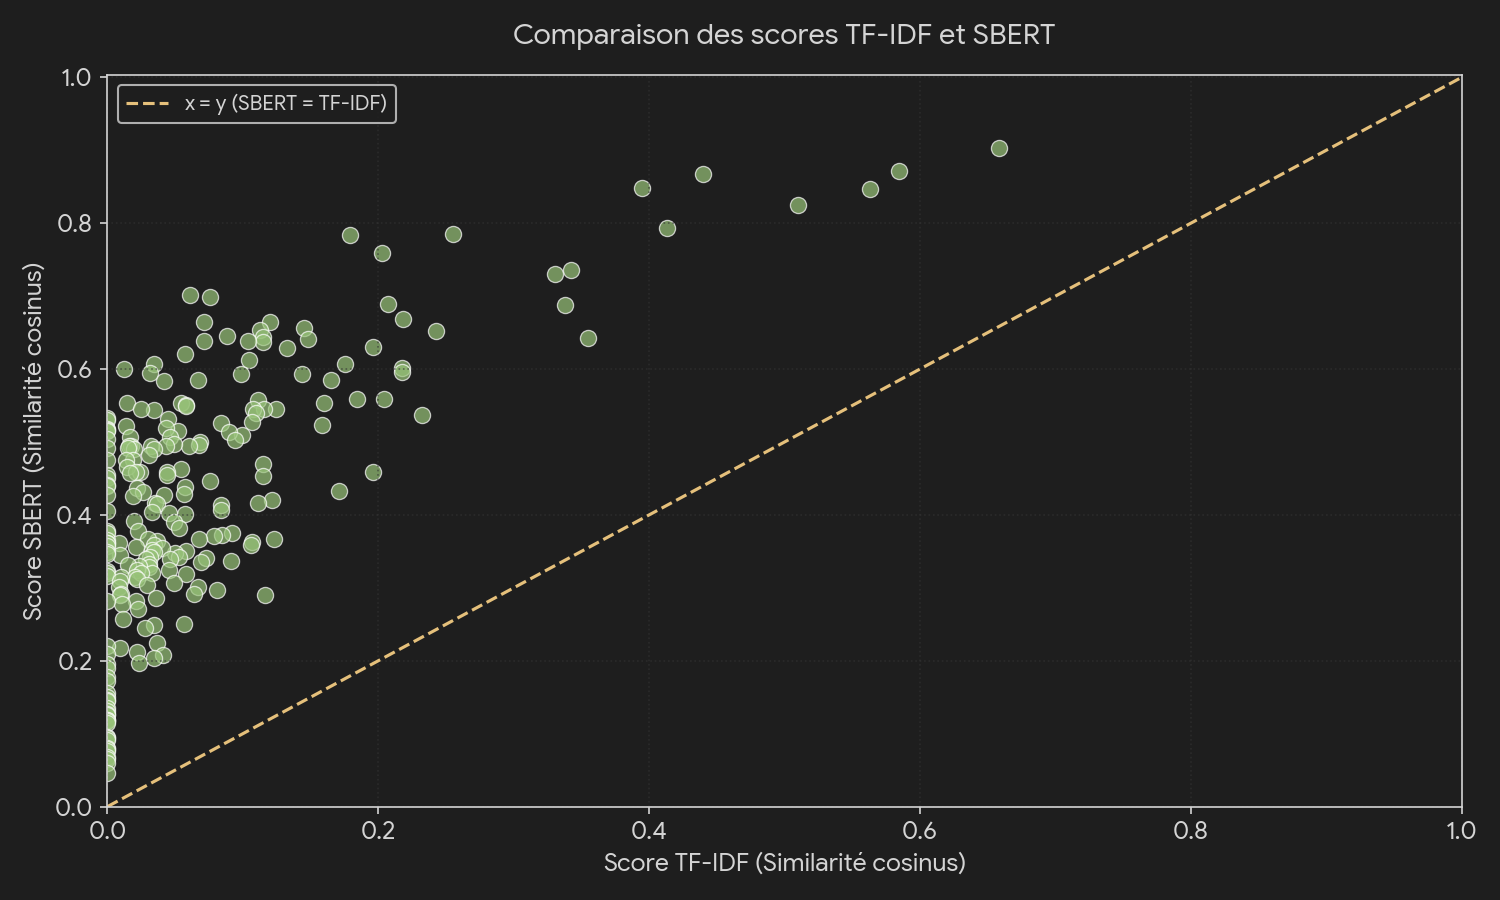
\includegraphics[width=0.8\textwidth]{TDF-IDF_SBERT.png}
\caption{Comparaison des scores de similarité cosinus TF--IDF et SBERT pour l'ensemble des paires d'énoncés. La ligne pointillée représente l'égalité des scores.}
\label{fig:tfidf_sbert}
\end{figure}

L'analyse de cette distribution confirme empiriquement les limites de ces approches textuelles. La quasi-totalité des points se situe au-dessus de la ligne d'égalité, démontrant que SBERT attribue des scores systématiquement plus élevés (moyenne de 0,42) que TF--IDF (moyenne de 0,07). L'importante dispersion verticale sur la gauche du graphique montre la capacité de SBERT à rapprocher des énoncés partageant une sémantique commune mais aucun vocabulaire (TF--IDF proche de 0). Cependant, l'absence de regroupements (clusters) distincts prouve que ces scores thématiques peinent à segmenter finement les exercices selon leur démarche de résolution algorithmique.

Pour illustrer concrètement ces limites, nous pouvons examiner un  cas représentatif tiré de notre corpus, mettant en évidence les \og illusions \fg{} lexicales :

\paragraph{Exemple : l'illusion lexicale (TF--IDF élevé, structures différentes).}
\begin{itemize}
\item \textit{Énoncé A :} \og Écrire un programme qui demande une somme cible entre 2 et 12, puis affiche toutes les combinaisons possibles de deux dés à six faces donnant cette somme. Afficher aussi le nombre total de combinaisons. \fg{}
\item \textit{Énoncé B :} \og Écrire un programme qui demande à l'utilisateur un nombre de dés (entre 1 et 8) et une somme cible. Le programme doit afficher combien de combinaisons de résultats permettent d'obtenir cette somme avec des dés à six faces. \fg{}
\end{itemize}

Pour cette paire, les deux méthodes accordent des scores très élevés (TF--IDF = 0,65 ; SBERT = 0,90) en raison du fort
champ lexical partagé (dés, somme, combinaisons). Pourtant, le premier énoncé se résout par de simples boucles imbriquées
fixes, tandis que le second requiert une approche récursive ou une gestion dynamique pour un nombre variable de dés.
Les métriques textuelles échouent à capturer cette rupture de complexité structurelle.

\paragraph{Comparaison de séquences de jetons (stratégie de JPlag).}

JPlag compare les programmes en deux étapes \cite{prechelt_finding_nodate}.
Chaque programme est d'abord transformé en une suite de jetons : les noms de
variables et les valeurs sont effacés, seuls restent des éléments comme
\og début de boucle \fg{} ou \og affectation \fg{}. Les deux suites sont
ensuite comparées en cherchant les plus longs morceaux identiques qu'elles
ont en commun (\emph{Greedy String Tiling}).

La première étape rejoint notre démarche : la normalisation de l'AST efface
elle aussi les noms et les valeurs. La seconde ne correspond pas à notre
objectif. JPlag cherche de longs passages identiques, signe qu'un programme
a été recopié. Or deux exercices substituables ne sont pas des copies : ils
suivent la même démarche avec une écriture qui peut varier. Remplacer une
boucle \texttt{for} par une boucle \texttt{while} ou changer l'ordre de deux
instructions suffit à couper la suite de jetons en petits morceaux, alors
que la démarche est inchangée. De plus, une suite de jetons est
\og à plat \fg{} : elle ne dit pas quelle instruction se trouve à
l'intérieur de quelle boucle, alors que cette imbrication décrit justement
la démarche de résolution. Nous avons donc gardé l'idée de normalisation,
mais remplacé la comparaison de séquences par une comparaison d'arbres.


 

\paragraph{Graphes de dépendances et modélisations hybrides (CFG, PDG, CPG, CSSG).}

Pour dépasser la rigidité topologique des Arbres Syntaxiques Abstraits (AST), la modélisation des flux d'exécution a été explorée afin de capturer l'essence sémantique du code. Contrairement à un AST qui décrit la forme syntaxique stricte, les graphes de flot de contrôle (CFG) modélisent les différents chemins d'exécution possibles, tandis que les graphes de dépendances de données (DDG) et de programme (PDG) explicitent les relations entre la définition d'une variable et ses utilisations ultérieures. Ces graphes présentent l'avantage majeur de rester stables même si un étudiant réordonne des instructions indépendantes ou modifie la syntaxe de surface.

Pour obtenir une représentation absolue, des approches hybrides telles que les CPG (Code Property Graphs) ou les CSSG (Code Syntax and Semantics Graphs) ont été étudiées. Le modèle CSSG, par exemple, fusionne l'AST, le CFG et le PDG en une structure de données unique, capturant simultanément la syntaxe et la sémantique d'exécution.

Cependant, cette piste s'est heurtée à un obstacle technique majeur lors de la phase de comparaison. Évaluer la similarité exacte entre deux graphes aussi riches et denses nécessite de calculer des distances d'édition de graphes (Graph Edit Distance) ou de rechercher des isomorphismes de sous-graphes. Ces opérations mathématiques étant d'une complexité algorithmique NP-difficile, le temps de calcul explose de manière exponentielle. Cette approche s'est donc révélée inapplicable pour évaluer et comparer à grande échelle un corpus important d'exercices en temps raisonnable. Elle demeure une perspective théorique d'enrichissement, mais a été écartée du pipeline principal.

\paragraph{Modèles appris et embeddings de code (CodeBERT et GraphCodeBERT).}

Face aux limites combinatoires des graphes, l'utilisation de modèles de langage pré-entraînés spécialisés dans le code source a été envisagée pour projeter les programmes dans un espace vectoriel dense (embeddings). Le modèle CodeBERT s'appuie sur une architecture Transformer entraînée conjointement sur du langage naturel et du code, tandis que son évolution, GraphCodeBERT, y intègre la structure du flux de données (data flow) pour mieux saisir la logique algorithmique sous-jacente.

Si ces modèles excellent dans la représentation globale du code, ils présentent une limite conceptuelle fondamentale par rapport à notre objectif. Ces architectures sont pré-entraînées sur des tâches de génie logiciel rudimentaires, telles que la recherche de code (Code Search) ou la détection binaire de clones (déterminer si un code A est le plagiat d'un code B). Par conséquent, les espaces vectoriels qu'ils génèrent sont optimisés pour la similarité fonctionnelle stricte, et échouent à mesurer la notion de substituabilité pédagogique.

Ces modèles ne parviennent pas à différencier un exercice dont la démarche de résolution est sémantiquement identique (et donc inutile à recommander à un étudiant qui maîtrise déjà le concept) d'un exercice partageant une thématique proche mais exigeant une structure de contrôle inédite (et donc pertinent pour la progression). Pour devenir exploitables dans un Environnement Informatique d'Apprentissage Humain (EIAH), ces modèles nécessiteraient un réentraînement profond (fine-tuning) sur de larges volumes de paires d'exercices annotées par des enseignants selon leur valeur d'apprentissage, une ressource actuellement indisponible à l'échelle requise. Ils ont donc été écartés au profit de représentations plus interprétables et ne nécessitant pas d'apprentissage préalable.

\paragraph{Apprentissage contrastif pour la similarité pédagogique.}

Pour lever l'obstacle des paires annotées, une méthode d'apprentissage
contrastif a été proposée. Elle s'inspire de BCRNet \cite{mu_2023} et des
travaux sur l'apprentissage contrastif d'images, de phrases et de code
\cite{chen_simclr_2020,gao_simcse_2021,jain_contracode_2021}. L'objectif est
d'apprendre une représentation vectorielle unique de chaque exercice, qui
réunit l'énoncé et la correction, sans recourir à des paires étiquetées
manuellement.

Pour chaque exercice, on génère deux \emph{vues} qui conservent le même
contenu pédagogique et le même comportement du code, mais dont la forme
diffère. Ces deux vues forment une \textbf{paire positive} que le modèle
apprend à rapprocher dans l'espace de représentation. Les vues des autres
exercices du lot d'entraînement forment des \textbf{paires négatives} que le
modèle apprend à éloigner, au moyen de la perte InfoNCE \cite{oord_infonce_2018}.
Le signal d'apprentissage vient donc uniquement de la structure du problème :
deux vues d'un même exercice doivent être proches. La méthode reposait sur
trois éléments :
\begin{itemize}
  \item \textbf{les vues de l'énoncé}, obtenues par \emph{dropout} appliqué à
        l'encodeur de texte, à la manière de SimCSE \cite{gao_simcse_2021}.
        Le masquage de mots utilisé par BCRNet a été écarté, car il fournit
        un signal faible à un modèle déjà pré-entraîné par masquage
        (\emph{masked language modeling}) ;
  \item \textbf{les vues de la correction}, obtenues par des transformations
        qui préservent la sémantique et que la littérature a déjà validées
        \cite{jain_contracode_2021,bui_corder_2021} : renommage des variables,
        suppression des commentaires, reformatage et réordonnancement
        d'instructions indépendantes ;
  \item \textbf{une fusion multimodale}, sur le modèle de BCRNet : l'énoncé
        et le code sont encodés séparément, leurs vecteurs sont concaténés,
        puis projetés dans un espace latent commun qui fournit un plongement
        unique par exercice.
\end{itemize}

Cette piste n'a pas été retenue, car elle repose sur deux types de paires
et nous ne pouvions en construire qu'un seul. Les paires positives sont faciles
à obtenir : il suffit de créer des variantes bruitées d'un même exercice.
Les paires négatives, en revanche, doivent être de vrais exemples
d'exercices \emph{non similaires}. Or, dans notre situation de démarrage à
froid, aucune annotation ne permet de savoir quels exercices sont différents.
Prendre simplement les autres exercices du lot comme négatifs reviendrait à
supposer qu'ils ne se ressemblent pas, alors que c'est justement ce que l'on
cherche à mesurer : deux exercices du corpus peuvent très bien être
similaires. Sans négatifs fiables, le modèle ne peut pas apprendre
correctement la notion de similarité.

L'idée des variantes bruitées a toutefois été conservée sous une autre
forme : les variantes contrôlées du chapitre~\ref{chap:resultats} ne servent
pas à entraîner un modèle, mais à \emph{vérifier} le comportement des mesures.

\paragraph{Fusion immédiate des signaux.}

Enfin, une fusion directe de toutes les mesures disponibles aurait pu produire
un score unique combinant texte, métriques, AST et structures de contrôle.
Cette solution aurait simplifié le classement des paires, mais elle aurait
également masqué la contribution de chaque représentation. Elle aurait en
outre nécessité de fixer des pondérations sans disposer d'une vérité terrain
ou de jugements d'enseignants pour les apprendre.

Pour cette raison, des méthodes sont d'abord étudiées séparément. Leurs
résultats pourront ensuite être comparés et combinés de manière explicite,
après analyse de leur comportement sur les variantes contrôlées. Ce choix
conduit au pipeline présenté dans le chapitre suivant. Celui-ci reposera sur
trois représentations complémentaires des corrections : des caractéristiques
globales du code, des arbres syntaxiques normalisés et une représentation
centrée sur l'organisation des structures de contrôle. Le nom, la construction
et le calcul précis de chacune de ces approches seront introduits au début du
chapitre suivant, avant la présentation de leurs résultats expérimentaux.
---


% =====================================================================
%  Chapitre : Ma proposition
%  Packages requis dans le préambule du document principal :
%    \usepackage[T1]{fontenc}
%    \usepackage[french]{babel}
%    \usepackage{amsmath,amssymb}
%    \usepackage{float}          % option [H]
%    \usepackage{booktabs,array,tabularx}
%    \usepackage{xcolor}
%    \usepackage{tikz}
%    \usetikzlibrary{arrows.meta,positioning,fit,backgrounds,calc,
%                    shapes.geometric,babel}
% =====================================================================

% ---------- Palette et styles communs à toutes les figures -----------
\definecolor{cEIIA}{HTML}{D9822B}   % orange : EIIA
\definecolor{cTSED}{HTML}{2D6DB5}   % bleu   : TSED
\definecolor{cNCST}{HTML}{2E8B57}   % vert   : NCST
\definecolor{cNeutre}{HTML}{5A6270} % gris   : étapes communes
\definecolor{cAlerte}{HTML}{C0392B} % rouge  : différences
\definecolor{cGrille}{HTML}{BFC4CC} % gris clair : repères

\tikzset{
  >=Stealth,
  fleche/.style={->, thick, draw=cNeutre},
  etape/.style={rectangle, rounded corners=3pt, draw=#1, thick,
    fill=#1!8, font=\sffamily\small, align=center,
    minimum height=0.9cm, text width=3.0cm, inner sep=4pt},
  etape/.default=cNeutre,
  donnee/.style={rectangle, draw=#1, thick, fill=white,
    font=\sffamily\small, align=center, minimum height=0.8cm,
    text width=2.8cm, inner sep=4pt,
    double, double distance=1pt},
  donnee/.default=cNeutre,
  scorebox/.style={rectangle, rounded corners=6pt, draw=#1, very thick,
    fill=#1!18, font=\sffamily\small\bfseries, align=center,
    minimum height=0.8cm, text width=2.6cm},
  cadre/.style={draw=#1, thick, rounded corners=6pt, fill=#1!4,
    inner sep=8pt},
  titrecadre/.style={font=\sffamily\footnotesize\bfseries, text=#1,
    fill=white, inner sep=2pt},
  noeud/.style={rectangle, rounded corners=2pt, draw=#1, thick,
    fill=#1!12, font=\sffamily\scriptsize, align=center,
    minimum height=0.55cm, minimum width=1.6cm, inner sep=2pt},
  noeud/.default=cNeutre,
  code/.style={rectangle, draw=cNeutre, thick, fill=gray!6,
    rounded corners=3pt, font=\ttfamily\scriptsize, align=left,
    inner sep=6pt},
  etiq/.style={font=\sffamily\scriptsize\itshape, text=cNeutre},
}



% =====================================================================
% Chapitre : Ma proposition (version mise à jour : NCST normalisé,
% appariement naïf ordonné et interface Streamlit)
% ---------------------------------------------------------------------
% Packages requis dans le préambule du rapport :
%   \usepackage[T1]{fontenc}
%   \usepackage[utf8]{inputenc}
%   \usepackage[french]{babel}
%   \usepackage{amsmath,amssymb}
%   \usepackage{booktabs,tabularx,array}
%   \usepackage{xcolor}
%   \usepackage{listings}
%   \usepackage{tikz}
%   \usetikzlibrary{positioning,arrows.meta,fit,calc,shapes.misc,backgrounds,babel}
%   (la bibliothèque TikZ « babel » est indispensable avec babel français)
% =====================================================================

% ---------- Couleurs et styles communs ----------
\definecolor{eiiacol}{RGB}{230,120,20}
\definecolor{tsedcol}{RGB}{30,90,180}
\definecolor{ncstcol}{RGB}{30,140,70}
\definecolor{uicol}{RGB}{120,60,160}
\definecolor{graycol}{RGB}{110,110,110}

\tikzset{
  box/.style={draw, rounded corners=2pt, align=center, font=\small,
    minimum height=0.8cm, inner sep=4pt, fill=white},
  frame/.style={draw, rounded corners=4pt, inner sep=8pt, thick},
  flow/.style={-{Stealth[length=2.2mm]}, thick},
  nnode/.style={draw=ncstcol, fill=ncstcol!10, rounded corners=1.5pt,
    font=\ttfamily\scriptsize, inner sep=2.5pt, minimum height=0.42cm,
    anchor=west},
  nlink/.style={draw=ncstcol!70!black, thin},
  elab/.style={font=\ttfamily\tiny, text=graycol, fill=white, inner sep=0.8pt},
  lvl/.style={font=\ttfamily\scriptsize, anchor=west},
}

\lstdefinestyle{pyncst}{
  language=Python, basicstyle=\ttfamily\small, keywordstyle=\color{tsedcol}\bfseries,
  commentstyle=\color{graycol}, frame=single, rulecolor=\color{ncstcol},
  framesep=4pt, xleftmargin=6pt, xrightmargin=6pt, showstringspaces=false,
  columns=fullflexible, keepspaces=true, backgroundcolor=\color{ncstcol!4}
}

\chapter{Ma proposition}

Ce chapitre présente le pipeline multi-niveaux développé pour évaluer la
substituabilité algorithmique entre des exercices de programmation. L'objectif
n'est pas de réduire la similarité à une seule propriété du code, mais de
comparer les corrections selon trois niveaux d'abstraction complémentaires : la
structure globale, la topologie syntaxique détaillée et l'organisation
structurelle abstraite du programme. Une interface Streamlit complète le
pipeline : elle permet de lancer les comparaisons, de consulter les trois
scores et d'inspecter les arbres produits à chaque étape.

% =====================================================================
\section{Architecture globale du pipeline}
% =====================================================================

Pour chaque paire de programmes $(A,B)$, le pipeline construit plusieurs
représentations du code et calcule trois mesures distinctes :
\begin{enumerate}
  \item l'\textbf{EIIA}, qui compare la difficulté global  extraits
        de l'AST normalisé ;
  \item le \textbf{TSED}, distance d'édition calculée sur des AST normalisés
        afin d'évaluer finement la topologie syntaxique ;
  \item le \textbf{NCST}, qui compare, par un appariement ordonné, les nœuds
        abstraits d'un arbre structurel normalisé.
\end{enumerate}

Ces trois mesures sont calculées séparément pour chaque paire. Le pipeline
produit donc trois scores indépendants, chacun décrivant une dimension
particulière de la ressemblance entre les programmes. Cette organisation
multi-vues permet notamment de repérer les cas où deux corrections ont une
complexité globale proche, mais des organisations structurelles différentes.
Elle est cohérente avec les travaux qui distinguent la similarité de contenu,
de structure et de finalité pédagogique~\cite{pelanek_2020,holyoak_surface_1987}.

La chaîne de traitement est résumée par la figure~\ref{fig:architecture}. Le
code source est d'abord analysé par Tree-sitter, qui produit un arbre
syntaxique concret (CST). Cet arbre alimente deux branches : la première le
convertit en AST simplifié puis le normalise, ce qui sert de base commune à
l'EIIA et au TSED ; la seconde construit directement le NCST brut à partir du
CST, le normalise puis apparie les nœuds abstraits. Les trois scores sont
exportés dans des colonnes séparées. L'interface Streamlit peut ensuite
calculer, à titre facultatif, un score pondéré dont les poids sont choisis par
l'utilisateur.

\begin{figure}[htbp]
\centering
\shorthandoff{:;!?}%
\resizebox{\textwidth}{!}{%
\begin{tikzpicture}[node distance=0.55cm and 0.7cm]
  % Tronc commun
  \node[box] (src) {Code source\\Python};
  \node[box, right=of src] (ts) {Analyse\\Tree-sitter};
  \node[box, right=of ts] (cst) {Arbre syntaxique\\concret (CST)};
  \draw[flow] (src) -- (ts);
  \draw[flow] (ts) -- (cst);
  \node[frame, draw=graycol, fit=(src)(ts)(cst),
        label={[font=\small\bfseries, text=graycol]above left:Tronc commun}] (trunk) {};

  % Branche AST
  \node[box, below=1.4cm of ts, xshift=-1.6cm] (conv) {Conversion\\CST $\rightarrow$ AST};
  \node[box, below=of conv] (astn) {Normalisation\\de l'AST};
  \node[box, below=of astn] (astnorm) {AST normalisé};
  \node[box, draw=eiiacol, below left=0.7cm and -0.6cm of astnorm] (eiia)
      {Profil structurel\\+ distance euclidienne};
  \node[box, draw=tsedcol, below right=0.7cm and -0.6cm of astnorm] (tsed)
      {Fonction principale ou module\\+ distance d'édition};
  \draw[flow] (conv) -- (astn);
  \draw[flow] (astn) -- (astnorm);
  \draw[flow, eiiacol] (astnorm) -- (eiia);
  \draw[flow, tsedcol] (astnorm) -- (tsed);
  \node[font=\bfseries, text=eiiacol, below=0.35cm of eiia] (seiia) {$S_{\mathrm{EIIA}}$};
  \node[font=\bfseries, text=tsedcol, below=0.35cm of tsed] (stsed) {$S_{\mathrm{TSED}}$};
  \draw[flow, eiiacol] (eiia) -- (seiia);
  \draw[flow, tsedcol] (tsed) -- (stsed);
  \node[frame, draw=tsedcol!70, fit=(conv)(astn)(astnorm)(eiia)(tsed)(seiia)(stsed),
        label={[font=\small\bfseries, text=tsedcol]above left:Branche AST (EIIA et TSED)}] (bast) {};

  % Branche NCST
  \node[box, draw=ncstcol, right=4.6cm of conv] (ncb) {Construction\\du NCST brut};
  \node[box, draw=ncstcol, below=of ncb] (ncn) {Normalisation\\structurelle};
  \node[box, draw=ncstcol, below=of ncn] (ncl) {Parcours en profondeur\\liste (kind, level)};
  \node[box, draw=ncstcol, below=0.7cm of ncl] (ncm) {Appariement\\naïf ordonné};
  \node[font=\bfseries, text=ncstcol, below=0.35cm of ncm] (sncst) {$S_{\mathrm{NCST}}$};
  \draw[flow, ncstcol] (ncb) -- (ncn);
  \draw[flow, ncstcol] (ncn) -- (ncl);
  \draw[flow, ncstcol] (ncl) -- (ncm);
  \draw[flow, ncstcol] (ncm) -- (sncst);
  \node[frame, draw=ncstcol!70, fit=(ncb)(ncn)(ncl)(ncm)(sncst),
        label={[font=\small\bfseries, text=ncstcol]above right:Branche NCST}] (bncst) {};

  \draw[flow] (cst.south) -- ++(0,-0.5) -| (conv.north);
  \draw[flow] (cst.south) -- ++(0,-0.5) -| (ncb.north);

  % Export et interface
  \node[box, below=1.0cm of stsed, xshift=1.8cm, text width=8.6cm] (csv)
     {\textbf{Export CSV} : \texttt{source\_a, source\_b, tsed\_similarity,}\\
      \texttt{eiia\_similarity, ncst\_similarity, error}\\
      {\footnotesize trois colonnes indépendantes}};
  \draw[flow, eiiacol] (seiia.south) |- (csv.west);
  \draw[flow, tsedcol] (stsed.south) -- (stsed.south |- csv.north);
  \draw[flow, ncstcol] (sncst.south) |- (csv.east);

  \node[box, draw=uicol, below=0.6cm of csv, text width=8.6cm] (ui)
     {\textbf{Interface Streamlit} : tableau des scores, score pondéré facultatif\\
      {\footnotesize (poids choisis par l'utilisateur), artefacts CST, AST, NCST}};
  \draw[flow, uicol] (csv) -- (ui);
\end{tikzpicture}%
}
\caption{Architecture globale du pipeline d'évaluation de la similarité
multi-niveaux. L'EIIA et le TSED partagent l'AST normalisé ; le NCST est
construit directement à partir du CST. L'interface Streamlit exploite le CSV
produit par le pipeline.}
\label{fig:architecture}
\end{figure}

Le tableau~\ref{tab:synthese} résume ce que chaque approche conserve, ignore
et mesure.

\begin{table}[htbp]
\centering
\small
\renewcommand{\arraystretch}{1.25}
\begin{tabularx}{\textwidth}{>{\bfseries}p{2.6cm}XXX}
\toprule
 & \textcolor{eiiacol}{EIIA} & \textcolor{tsedcol}{TSED} & \textcolor{ncstcol}{NCST} \\
\midrule
Représentation & AST normalisé, résumé en vecteur & AST normalisé complet &
  NCST normalisé, linéarisé en liste $(\mathit{kind},\mathit{level})$ \\
Information conservée & Effectifs de nœuds et profondeur &
  Labels AST, opérateurs, ordre et hiérarchie &
  Catégories structurelles, niveau d'imbrication, ordre du parcours \\
Information ignorée & Position et agencement des nœuds &
  Noms et valeurs concrètes &
  Noms, valeurs, expressions, opérateurs, paramètres, noms de fonctions \\
Calcul & Distance euclidienne normalisée &
  Distance d'édition de Zhang-Shasha &
  Appariement naïf ordonné, indice de Sørensen-Dice \\
Question posée & Les programmes ont-ils une taille et une complexité
  comparables ? & Les arbres sont-ils proches nœud à nœud ? &
  Les programmes partagent-ils les mêmes catégories abstraites aux mêmes
  niveaux, dans le même ordre ? \\
\bottomrule
\end{tabularx}
\caption{Synthèse des trois niveaux de représentation du pipeline.}
\label{tab:synthese}
\end{table}

% =====================================================================
\section{Évaluation de l'information indépendante de l'arbre (EIIA)}
% =====================================================================

L'EIIA fournit une mesure macroscopique de la proximité entre deux programmes.
Elle repose sur un profil structurel extrait en parcourant l'ensemble des
nœuds de l'AST normalisé. Pour un programme $A$, le profil est représenté par
le vecteur à neuf composantes :
\begin{equation}
V_A = (n_{nodes}, n_{operators}, n_{operands}, n_{assignments},
       n_{selections}, n_{iterations}, d_{max}, n_{calls}, n_{returns}).
\end{equation}

Le tableau~\ref{tab:eiia} précise les types de nœuds comptés pour chaque
composante.

\begin{table}[htbp]
\centering
\small
\begin{tabular}{lll}
\toprule
\textbf{Composante} & \textbf{Signification} & \textbf{Nœuds comptés} \\
\midrule
\texttt{n\_nodes} & taille de l'arbre & tous les nœuds \\
\texttt{n\_operators} & opérateurs & \texttt{BINARY\_OP, COMPARE, BOOLEAN\_OP, UNARY\_OP} \\
\texttt{n\_operands} & opérandes & \texttt{IDENTIFIER, NUMBER, STRING, BOOLEAN, NULL} \\
\texttt{n\_assignments} & affectations & \texttt{ASSIGN, AUG\_ASSIGN} \\
\texttt{n\_selections} & sélections & \texttt{IF, ELIF, ELSE, TERNARY} \\
\texttt{n\_iterations} & répétitions & \texttt{FOR, WHILE} \\
\texttt{d\_max} & profondeur maximale & --- \\
\texttt{n\_calls} & appels de fonction & \texttt{CALL} \\
\texttt{n\_returns} & retours & \texttt{RETURN} \\
\bottomrule
\end{tabular}
\caption{Composantes du profil structurel utilisé par l'EIIA.}
\label{tab:eiia}
\end{table}

La distance euclidienne entre les profils de deux programmes est définie par :
\begin{equation}
d(V_A,V_B) = \lVert V_A - V_B \rVert_2 .
\end{equation}
Cette distance est normalisée par la norme maximale des deux profils :
\begin{equation}
d_{norm}(A,B) = \frac{d(V_A,V_B)}{\max\left(\lVert V_A\rVert_2,
\lVert V_B\rVert_2, \varepsilon\right)}, \qquad \varepsilon = 10^{-12}.
\end{equation}
Le score EIIA est alors obtenu par :
\begin{equation}
S_{\mathrm{EIIA}}(A,B) = \max\left(0,\, 1 - d_{norm}(A,B)\right).
\end{equation}

La figure~\ref{fig:eiia} illustre cette chaîne de calcul. Aucune pondération
explicite n'est appliquée aux composantes. Cette décision ne signifie toutefois
pas qu'elles ont la même influence : les composantes conservant leurs échelles
brutes, les effectifs de nœuds peuvent dominer les composantes moins fréquentes,
comme la profondeur ou le nombre de retours. Cette limite est prise en compte
dans l'interprétation de l'EIIA.

\begin{figure}[htbp]
\centering
\shorthandoff{:;!?}%
\resizebox{\textwidth}{!}{%
\begin{tikzpicture}[node distance=0.5cm and 0.6cm]
  \node[box] (a) {AST normalisé\\de $A$};
  \node[box, below=0.6cm of a] (b) {AST normalisé\\de $B$};
  \node[box, draw=eiiacol, right=1.7cm of a] (va) {$V_A \in \mathbb{N}^9$};
  \node[box, draw=eiiacol, right=1.7cm of b] (vb) {$V_B \in \mathbb{N}^9$};
  \draw[flow] (a) -- node[above, font=\scriptsize]{comptage} (va);
  \draw[flow] (b) -- node[above, font=\scriptsize]{comptage} (vb);
  \node[frame, draw=eiiacol!70, fit=(a)(b)(va)(vb),
        label={[font=\small\bfseries, text=eiiacol]above:1. Extraction des profils}] (f1) {};

  \node[box, draw=eiiacol, right=1.6cm of $(va)!0.5!(vb)$] (d) {$d = \lVert V_A - V_B\rVert_2$};
  \node[box, draw=eiiacol, right=of d] (dn) {$d_{norm} = \dfrac{d}{\max(\lVert V_A\rVert_2,\lVert V_B\rVert_2,\varepsilon)}$};
  \node[box, draw=eiiacol, fill=eiiacol!10, right=of dn] (s) {$S_{\mathrm{EIIA}} = \max(0, 1 - d_{norm})$};
  \draw[flow] (va.east) -- (d.west);
  \draw[flow] (vb.east) -- (d.west);
  \draw[flow] (d) -- (dn);
  \draw[flow] (dn) -- (s);
  \node[font=\scriptsize, text=graycol, below=0.15cm of s] {score borné dans $[0,1]$};
  \node[frame, draw=eiiacol!70, fit=(d)(dn)(s), inner sep=10pt,
        label={[font=\small\bfseries, text=eiiacol]above:2. Comparaison non pondérée}] {};
\end{tikzpicture}%
}
\caption{Chaîne de calcul de l'EIIA : extraction de deux profils structurels,
puis distance euclidienne normalisée.}
\label{fig:eiia}
\end{figure}

Cette approche s'inscrit dans la famille des métriques statiques qui décrivent
la taille et la complexité d'un programme sans nécessiter l'alignement de deux
arbres ou graphes~\cite{vujosevic-janicic_software_2013}. Des travaux consacrés à l'évaluation de la
difficulté et de l'effort de programmation montrent également que des
métriques telles que la taille du code et la complexité cyclomatique peuvent
être corrélées à un indice d'effort interne, l'\emph{Index of Internal Effort}
(IIE)~\cite{de_oliveira_assessing_2024}. Cette observation soutient l'utilisation de profils
quantitatifs comme indicateurs de complexité, sans établir pour autant une
équivalence entre l'EIIA et l'IIE. L'EIIA constitue ainsi un indicateur de la
proximité globale d'architecture et de complexité, sans prétendre décrire à
lui seul la stratégie algorithmique détaillée : deux programmes ayant les
mêmes effectifs de nœuds obtiennent un score maximal même si ces nœuds sont
agencés différemment.

% =====================================================================
\section{AST normalisé et distance TSED}
% =====================================================================

La deuxième approche évalue la structure grammaticale détaillée du code. Le
code Python est d'abord analysé avec Tree-sitter, puis converti en un AST
simplifié dont les nœuds portent des types unifiés (\texttt{FUNCTION},
\texttt{ASSIGN}, \texttt{IF}, \texttt{FOR}, \texttt{BINARY\_OP}, \texttt{CALL},
\texttt{IDENTIFIER}, etc.). Une phase de normalisation réduit ensuite
l'influence des choix de style et des détails formels qui ne modifient pas la
logique de résolution.

\subsection{Conversion du CST en AST simplifié}
\label{sec:conversion_ast}

La conversion parcourt les nœuds nommés du CST et associe à chaque type
Tree-sitter un type de l'AST interne au moyen d'une table de correspondance.
Les nœuds anonymes (mots-clés, ponctuation) ne sont pas conservés, à
l'exception des opérateurs, qui sont recopiés comme valeur du nœud
(\texttt{BINARY\_OP(+)}, \texttt{COMPARE(==)}, \texttt{UNARY\_OP(not)}).

Une table de correspondance ne couvre jamais toute la grammaire du
langage, et le traitement des types absents influe directement sur les
mesures. Leur attribuer un label générique commun, par exemple
\texttt{UNKNOWN}, rendrait identiques des constructions sans rapport : pour
le TSED, une compréhension de liste, une négation \texttt{not}, une tranche
\texttt{l[1:3]} ou une définition de classe deviendraient des nœuds
substituables à coût nul. Sur le corpus GitHub, ces constructions sont
fréquentes : on y compte notamment 23 compréhensions de liste, 13
définitions de classe, 8 négations et 7 tranches.

Plutôt que de chercher à couvrir toute la grammaire de Python, la conversion
applique quatre règles simples (tableau~\ref{tab:kind_map}) :
\begin{itemize}
  \item \textbf{types ajoutés à la table} : une construction ne reçoit son
        propre type que si elle traduit un choix de résolution. Par exemple,
        filtrer une liste avec une boucle \texttt{for} ou avec la
        compréhension \texttt{[x for x in liste if x \% 2 == 0]} sont deux
        démarches différentes : la compréhension reçoit donc le type
        \texttt{LIST\_COMP}, pour que les mesures puissent les distinguer.
        Son \texttt{for} et son \texttt{if} sont en revanche typés
        \texttt{FOR} et \texttt{IF}, comme une boucle et un test ordinaires,
        puisqu'ils réalisent eux aussi une itération et une sélection. Le
        même raisonnement s'applique à la négation (\texttt{not x}), aux
        tranches (\texttt{l[1:]}) et aux classes. Les tuples
        (\texttt{a, b}) et les paires clé-valeur (\texttt{k: v}) reçoivent
        aussi un type, afin que les valeurs qu'ils regroupent ne se mélangent
        pas avec les nœuds voisins ;
  \item \textbf{feuilles} : une chaîne de caractères et un import ne gardent
        aucun enfant, quel que soit leur découpage interne par l'analyseur.
        Toute instruction qui commence par \texttt{import} ou
        \texttt{from}, quelle que soit sa forme (alias, nom pointé, import
        relatif ou \texttt{*}), devient un unique nœud \texttt{IMPORT} : seule
        la présence de l'import compte, pas le module importé. Le NCST
        applique déjà ce principe, chaque import y formant un seul nœud
        \texttt{STATEMENT} ;
  \item \textbf{paramètres réduits à leur nom} : quelle que soit sa forme
        (\texttt{n=2}, \texttt{n: int}, \texttt{*args}, \texttt{**kwargs}),
        un paramètre devient un nœud \texttt{IDENTIFIER}. Le nombre et
        l'ordre des paramètres sont conservés, ce qui suffit à
        l'anonymisation en \texttt{PARAM\_1}, \texttt{PARAM\_2}, etc. ; les
        valeurs par défaut et les annotations de type relèvent du style et
        non de la stratégie ;
  \item \textbf{suppression des nœuds non reconnus} : un nœud dont le type
        est absent de la table n'est pas conservé et ses enfants prennent
        directement sa place. Les constructions rares (\texttt{with \dots\ as},
        \texttt{match}, décorateurs, etc.) gardent ainsi leur contenu
        (appels, identifiants, blocs) sans introduire d'étiquette
        artificielle. Par exemple, pour une fonction décorée par
        \texttt{@cache}, l'AST contient directement
        \texttt{IDENTIFIER(cache)} suivi de \texttt{FUNCTION}. Les
        déclarations \texttt{global} et \texttt{nonlocal} sont ignorées.
\end{itemize}

La suppression d'un nœud non reconnu préserve l'ordre de l'arbre : ses
enfants sont insérés exactement à sa position, entre ses voisins, qui ne
sont pas déplacés. La règle s'applique récursivement, si bien que plusieurs
niveaux non reconnus successifs disparaissent ensemble. Dans l'exemple de la
figure~\ref{fig:unknown_splice}, chaque appel de l'instruction
\texttt{with} est emboîté dans trois nœuds intermédiaires qui disparaissent
ensemble ; le contenu et son ordre sont conservés, ce qui importe pour le
TSED, et les instructions voisines \texttt{a = 1} et \texttt{return a}
restent à leur place.

\begin{figure}[htbp]
\centering
\small
\begin{minipage}[t]{0.30\textwidth}
\textbf{Code}
\begin{verbatim}
def f(p):
    a = 1
    with open(p) as fh, \
         open("y") as g:
        b = 2
    return a
\end{verbatim}
\end{minipage}\hfill
\begin{minipage}[t]{0.36\textwidth}
\textbf{CST Tree-sitter (extrait)}
\begin{verbatim}
block
  assignment          a = 1
  with_statement
    with_clause     (x)
      with_item     (x)
        as_pattern  (x)
          call        open(p)
          identifier  fh
      with_item     (x)
        as_pattern  (x)
          call        open("y")
          identifier  g
    block             b = 2
  return_statement    return a
\end{verbatim}
\end{minipage}\hfill
\begin{minipage}[t]{0.30\textwidth}
\textbf{AST obtenu}
\begin{verbatim}
BLOCK
  ASSIGN       a = 1
  WITH
    CALL       open(p)
    IDENTIFIER(fh)
    CALL       open("y")
    IDENTIFIER(g)
    BLOCK      b = 2
  RETURN       return a
\end{verbatim}
\end{minipage}
\caption{Suppression des nœuds non reconnus, marqués \texttt{(x)} : leurs
enfants prennent leur place dans le même ordre, et les instructions voisines
ne sont pas déplacées. Le nœud \texttt{as\_pattern\_target} qui entoure
\texttt{fh} et \texttt{g} est omis de l'extrait ; il est supprimé de la même
manière.}
\label{fig:unknown_splice}
\end{figure}

Avec ces règles, l'AST ne contient aucun nœud \texttt{UNKNOWN}, par
construction. Les conséquences de la suppression des nœuds non reconnus sont
discutées dans les limites (section~\ref{sec:limites_conversion}).

\begin{table}[htbp]
\centering
\small
\renewcommand{\arraystretch}{1.2}
\begin{tabularx}{\textwidth}{>{\bfseries}p{3.0cm}X}
\toprule
Règle & Effet sur l'AST (exemple de code) \\
\midrule
Types ajoutés &
  \texttt{LIST\_COMP}, \texttt{DICT\_COMP}, \texttt{SET\_COMP},
  \texttt{GENERATOR}, dont le \texttt{for} et le \texttt{if} sont typés
  \texttt{FOR} et \texttt{IF} (\texttt{[x for x in l if c]}) ; \texttt{UNARY\_OP(not)} ;
  \texttt{SLICE} (\texttt{l[1:3]}) ; \texttt{PAIR} (\texttt{k: v}) ;
  \texttt{TUPLE} (\texttt{a, b = b, a}) ; \texttt{CLASS} \\
Feuilles &
  \texttt{STRING} sans enfant ;
  \texttt{IMPORT} sans enfant pour \texttt{import os.path as osp},
  \texttt{from math import *}, etc. \\
Paramètres &
  \texttt{def f(l, n: int = 2, *a, **k)} $\rightarrow$
  \texttt{PARAMETERS(l, n, a, k)}, y compris pour une \texttt{lambda} \\
Nœuds supprimés &
  type absent de la table : remplacé par ses enfants ;
  \texttt{global} et \texttt{nonlocal} : ignorés \\
\bottomrule
\end{tabularx}
\caption{Règles de conversion du CST Tree-sitter en AST interne. Aucun nœud
\texttt{UNKNOWN} n'est produit.}
\label{tab:kind_map}
\end{table}

Pour l'EIIA (tableau~\ref{tab:eiia}), le \texttt{for} et le \texttt{if}
d'une compréhension sont donc comptés comme une itération et une sélection,
et la négation \texttt{not}, typée \texttt{UNARY\_OP}, est comptée parmi les
opérateurs.

\subsection{Normalisation de l'AST}

La normalisation transforme les deux arbres avant le calcul de la distance
d'édition. Elle comprend les opérations suivantes :
\begin{itemize}
  \item l'anonymisation canonique des paramètres, des variables locales et des
        fonctions du fichier, remplacés dans l'ordre d'apparition par
        \texttt{PARAM\_1}, \texttt{VAR\_1} et \texttt{FUNC\_1} ;
  \item l'abstraction des littéraux, qui remplace les valeurs concrètes par les
        catégories \texttt{NUM}, \texttt{STR}, \texttt{BOOL} et \texttt{NULL} ;
  \item l'\emph{inlining} des fonctions auxiliaires simples. L'appel est
        remplacé par l'expression renvoyée par la fonction, dans laquelle
        chaque paramètre est remplacé par l'argument correspondant. Par
        exemple, avec \texttt{def est\_pair(n): return n \% 2 == 0},
        l'appel \texttt{if est\_pair(x):} devient \texttt{if x \% 2 == 0:}.
        Le corps de la fonction n'est donc pas recopié à l'endroit de
        l'appel : seule son expression de retour est substituée. Cette
        substitution n'est appliquée qu'aux fonctions définies dans le même
        fichier et dont le corps se réduit à un unique \texttt{return}
        portant une expression, sans affectation, boucle, condition, appel,
        exception ni récursion. Les fonctions prédéfinies du langage, comme
        \texttt{sum} ou \texttt{len}, et les fonctions importées ne sont
        jamais remplacées : leur appel reste un nœud \texttt{CALL}.
\end{itemize}

Les opérateurs, tels que \texttt{+}, \texttt{\%} ou \texttt{==}, ainsi que les
structures de contrôle sont conservés, car ils portent une information
importante sur la stratégie de résolution. Les affectations augmentées, comme
\texttt{a += b}, sont conservées telles quelles : elles ne sont pas confondues
avec l'affectation explicite \texttt{a = a + b}. Les commentaires sont
supprimés dès la conversion de l'arbre. La figure~\ref{fig:astnorm} illustre l'effet combiné
de ces règles sur une instruction.

\begin{figure}[htbp]
\centering
\shorthandoff{:;!?}%
\resizebox{\textwidth}{!}{%
\begin{tikzpicture}[
  t/.style={draw, rounded corners=1.5pt, font=\ttfamily\scriptsize, inner sep=3pt},
  bad/.style={t, draw=red!70!black, fill=red!8},
  good/.style={t, draw=ncstcol, fill=ncstcol!10},
  level distance=1.1cm]
  % Avant
  \node[font=\bfseries] at (0,1.6) {Avant};
  \node[font=\ttfamily\small, align=left] at (0,0.8)
       {\textcolor{red!70!black}{\# cumul}\\total += x * 2};
  \node[t] (r1) at (0,-0.4) {AUG\_ASSIGN(+=)}
    [sibling distance=2.6cm]
    child {node[bad] {IDENTIFIER(total)}}
    child {node[t] {BINARY\_OP(*)}
      [sibling distance=2.0cm]
      child {node[bad] {IDENTIFIER(x)}}
      child {node[bad] {NUMBER(2)}}};
  % Règles
  \node[box, draw=graycol, font=\scriptsize, align=left] (rules) at (4.6,-1.0)
    {\textbf{Règles appliquées}\\
     commentaire supprimé\\
     \texttt{total} $\rightarrow$ \texttt{VAR\_1}\\
     \texttt{x} $\rightarrow$ \texttt{VAR\_2}\\
     \texttt{2} $\rightarrow$ \texttt{NUM}\\
     opérateurs conservés};
  \draw[flow, graycol] (2.6,-1.0) -- (rules.west);
  \draw[flow, graycol] (rules.east) -- (6.8,-1.0);
  % Après
  \node[font=\bfseries] at (9.6,1.6) {Après};
  \node[font=\ttfamily\small] at (9.6,0.8) {VAR\_1 += VAR\_2 * NUM};
  \node[t] at (9.6,-0.4) {AUG\_ASSIGN(+=)}
    [sibling distance=2.8cm]
    child {node[good] {IDENTIFIER(VAR\_1)}}
    child {node[t] {BINARY\_OP(*)}
      [sibling distance=2.5cm]
      child {node[good] {IDENTIFIER(VAR\_2)}}
      child {node[good] {NUMBER(NUM)}}};
\end{tikzpicture}%
}
\caption{Normalisation d'une instruction. Les nœuds en rouge portent des
détails de surface (noms, valeurs) ; après normalisation, ils sont remplacés
par des formes canoniques (en vert). Les opérateurs et la forme de
l'affectation sont conservés.}
\label{fig:astnorm}
\end{figure}

\subsection{Distance d'édition entre arbres}

La distance TSED correspond à la distance d'édition entre les deux arbres
normalisés, calculée selon l'algorithme de Zhang et
Shasha~\cite{zhang_simple_1989}. Chaque nœud est décrit par un label
associant son type à sa valeur résiduelle, par exemple \texttt{BINARY\_OP(+)}
ou \texttt{IDENTIFIER(VAR\_1)}. Les coûts d'insertion, de suppression et de
substitution sont unitaires :
\begin{equation}
c_{ins} = c_{del} = 1, \qquad
c_{sub}(u,v) =
\begin{cases}
0 & \text{si } \mathrm{label}(u) = \mathrm{label}(v),\\
1 & \text{sinon.}
\end{cases}
\end{equation}

Si $TED(A,B)$ désigne la distance d'édition et $|A|$ et $|B|$ le nombre de
nœuds des deux arbres, le score est défini par :
\begin{equation}
S_{\mathrm{TSED}}(A,B) = 1 - \frac{TED(A,B)}{|A| + |B|}.
\end{equation}
Le dénominateur est la seule borne valable pour toute paire d'arbres :
supprimer tous les nœuds de $A$ puis insérer tous ceux de $B$ coûte
$|A| + |B|$. La distance peut en revanche dépasser $\max(|A|,|B|)$, car une
substitution ne modifie que le label d'un nœud, jamais la forme de l'arbre.
Lorsque les formes diffèrent, un nœud mal placé ne peut pas être renommé : il
doit être supprimé puis recréé, soit deux opérations. Par exemple, une chaîne
de quatre nœuds et un arbre formé d'une racine et de trois feuilles sont à une
distance de 6. Ce dénominateur garantit un score compris entre 0 et 1.

La figure~\ref{fig:tsed} montre un cas minimal : deux fonctions qui ne
diffèrent que par un opérateur. Une seule substitution suffit à transformer un
arbre en l'autre.

\begin{figure}[htbp]
\centering
\begin{tikzpicture}[
  t/.style={draw=tsedcol, fill=tsedcol!8, rounded corners=1.5pt,
            font=\ttfamily\scriptsize, inner sep=3pt},
  hl/.style={t, draw=red!70!black, fill=red!8, thick},
  level distance=1.0cm, sibling distance=3.3cm]
  \node[font=\ttfamily\small] at (0,0.8) {return a + b};
  \node[t] at (0,0) {RETURN}
    child {node[hl] (opA) {BINARY\_OP(+)}
      child {node[t] {IDENTIFIER(PARAM\_1)}}
      child {node[t] {IDENTIFIER(PARAM\_2)}}};
  \node[font=\ttfamily\small] at (8.5,0.8) {return a * b};
  \node[t] at (8.5,0) {RETURN}
    child {node[hl] (opB) {BINARY\_OP(*)}
      child {node[t] {IDENTIFIER(PARAM\_1)}}
      child {node[t] {IDENTIFIER(PARAM\_2)}}};
  \draw[flow, red!70!black, dashed] (opA) -- node[above, font=\scriptsize]{substitution, coût 1} (opB);
  \node[draw=tsedcol, rounded corners, fill=tsedcol!5, inner sep=5pt] at (4.25,-3.2)
     {$TED = 1,\quad |A| = |B| = 4 \quad\Rightarrow\quad S_{\mathrm{TSED}} = 1 - \frac{1}{4 + 4} = 0{,}875$};
\end{tikzpicture}
\caption{Exemple de calcul TSED sur deux AST normalisés de quatre nœuds.}
\label{fig:tsed}
\end{figure}

Pour comparer des arbres de même niveau, le système choisit, pour chaque
paire, l'arbre comparé selon la présence de fonctions. Si les deux fichiers
contiennent des fonctions, la comparaison porte sur leur fonction
principale, celle dont l'AST contient le plus de nœuds (la première en cas
d'égalité), afin de comparer en priorité la fonction centrale de la
correction. Si au moins l'un des deux fichiers n'en contient aucune, comme un
script écrit au niveau du module, la comparaison porte sur le module complet
des deux fichiers : une fonction n'est ainsi jamais confrontée à un module
entier. L'EIIA est calculé sur le même arbre ; le NCST porte toujours sur le
fichier entier.

% =====================================================================
\section{Arbre structurel normalisé (NCST)}
% =====================================================================

La troisième approche compare l'organisation structurelle abstraite des
programmes. Deux AST peuvent être très différents tout en présentant une
organisation proche lorsqu'ils partagent les mêmes catégories de blocs, aux
mêmes niveaux d'imbrication et dans le même ordre.

\subsection{Construction et normalisation du NCST}

Le NCST (\emph{Normalized Control Structure Tree}) est d'abord construit sous
forme brute directement à partir du CST produit par Tree-sitter. Les
instructions sont regroupées en séquences et chaque construction structurante
devient un nœud typé, relié à ses blocs par des arêtes étiquetées.

La construction suit trois règles complémentaires :
\begin{itemize}
  \item les commentaires et les décorateurs ne produisent aucun nœud : une
        fonction décorée est construite comme une fonction ordinaire ;
  \item une sélection reçoit une branche par alternative : chaque
        \texttt{elif} forme une branche \texttt{ELIF} avec son propre bloc,
        suivie de l'éventuelle branche \texttt{ELSE} ;
  \item les compréhensions et les fonctions anonymes, bien qu'elles soient
        des expressions, reçoivent un nœud propre, \texttt{COMPREHENSION} ou
        \texttt{LAMBDA}, placé sous l'instruction qui les contient. Les quatre
        formes de compréhension de Python (liste, dictionnaire, ensemble et
        expression génératrice) partagent le même type. Ce nœud signale la
        présence de la construction sans en décrire le contenu.
\end{itemize}

Une normalisation structurelle est ensuite appliquée. Elle supprime toutes les
informations dépendantes du code source :
\begin{itemize}
  \item les noms des variables ;
  \item les valeurs constantes ;
  \item les expressions ;
  \item les opérateurs ;
  \item les paramètres ;
  \item les noms exacts des fonctions.
\end{itemize}

Seules les catégories et les relations structurelles sont conservées
(tableau~\ref{tab:ncst_vocab}). Contrairement à une simple extraction des
structures de contrôle, les instructions ordinaires restent présentes sous la
forme de nœuds anonymes \texttt{STATEMENT} : le NCST normalisé conserve donc
la présence et la position des instructions, sans leur contenu.

\begin{table}[htbp]
\centering
\small
\renewcommand{\arraystretch}{1.2}
\begin{tabularx}{\textwidth}{>{\bfseries}p{3.2cm}X}
\toprule
Catégories conservées &
\texttt{PROGRAM}, \texttt{CLASS}, \texttt{FUNCTION}, \texttt{SEQUENCE},
\texttt{ITERATION}, \texttt{SELECTION}, \texttt{EXCEPTION}, \texttt{HANDLER},
\texttt{CONTEXT}, \texttt{COMPREHENSION}, \texttt{LAMBDA}, \texttt{TRANSFER},
\texttt{STATEMENT} \\
\midrule
Relations conservées &
\texttt{BODY}, \texttt{CONTAINS}, \texttt{NEXT}, \texttt{THEN}, \texttt{ELSE},
\texttt{ELIF}, \texttt{CASE}, \texttt{DEFAULT}, \texttt{TRY}, \texttt{CATCH},
\texttt{FINALLY} \\
\midrule
Informations supprimées &
noms de variables, constantes, expressions, opérateurs, paramètres, noms
exacts des fonctions \\
\bottomrule
\end{tabularx}
\caption{Vocabulaire du NCST normalisé.}
\label{tab:ncst_vocab}
\end{table}

\subsection{Niveau structurel}

Chaque nœud reçoit un niveau structurel (\emph{level}) qui représente son
niveau d'imbrication. Les relations qui ouvrent un bloc (\texttt{BODY},
\texttt{THEN}, \texttt{ELSE}, \texttt{ELIF}, \texttt{CASE}, \texttt{DEFAULT},
\texttt{TRY}, \texttt{CATCH}, \texttt{FINALLY}) augmentent le niveau ; les
relations \texttt{CONTAINS} et \texttt{NEXT} conservent le niveau courant
(figure~\ref{fig:levels}). Le niveau structurel n'est donc pas la profondeur
de l'arbre : un nœud \texttt{FUNCTION} contenu dans la séquence racine reste
au même niveau que cette séquence.

\begin{figure}[htbp]
\centering
\begin{tikzpicture}
  \node[box, draw=ncstcol] (p) at (0,0) {nœud parent\\niveau $\ell$};
  \node[box, draw=ncstcol] (c1) at (-4.2,-2.6) {nœud enfant\\niveau $\ell$};
  \node[box, draw=ncstcol, fill=ncstcol!10] (c2) at (4.2,-2.6) {nœud enfant\\niveau $\ell+1$};
  \draw[flow, graycol] (p) -- node[above left=2pt, font=\ttfamily\scriptsize, align=center]{CONTAINS\\NEXT} (c1);
  \draw[flow, ncstcol] (p) -- node[above right=2pt, font=\ttfamily\scriptsize, align=center]
      {BODY, THEN, ELIF,\\ELSE, CASE, DEFAULT,\\TRY, CATCH, FINALLY} (c2);
  \node[font=\small\itshape, below=0.2cm of c1] {même niveau};
  \node[font=\small\itshape, below=0.2cm of c2] {entrée dans un bloc};
\end{tikzpicture}
\caption{Calcul du niveau structurel dans le NCST : seules les arêtes qui
ouvrent un bloc incrémentent le niveau.}
\label{fig:levels}
\end{figure}

La normalisation conserve les imbrications. Une sélection placée dans une
itération et une itération placée dans une sélection produisent deux arbres
distincts (figure~\ref{fig:imbrication}) : la normalisation ne confond pas ces
deux situations.

\begin{figure}[htbp]
\centering
\begin{tikzpicture}[x=0.5cm, y=-0.58cm]
  % Cas 1 : sélection dans une itération
  \node[font=\small\bfseries] at (3.5,-1.4) {Sélection dans une itération};
  \node[nnode] (a1) at (0,0) {ITERATION};
  \node[nnode] (a2) at (1,1) {SEQUENCE};
  \node[nnode] (a3) at (2,2) {SELECTION};
  \node[nnode] (a4) at (3,3) {SEQUENCE};
  \node[nnode] (a5) at (4,4) {STATEMENT};
  \foreach \pp/\cc in {a1/a2,a2/a3,a3/a4,a4/a5}
     \draw[nlink] ($(\pp.south west)+(0.25,0)$) |- (\cc.west);
  \node[font=\ttfamily\scriptsize, align=left, anchor=north west] at (0,5.2)
    {[(ITERATION,0), (SEQUENCE,1),\\ \ (SELECTION,1), (SEQUENCE,2),\\ \ (STATEMENT,2)]};

  % Cas 2 : itération dans une sélection
  \begin{scope}[xshift=7.2cm]
  \node[font=\small\bfseries] at (3.5,-1.4) {Itération dans une sélection};
  \node[nnode] (b1) at (0,0) {SELECTION};
  \node[nnode] (b2) at (1,1) {SEQUENCE};
  \node[nnode] (b3) at (2,2) {ITERATION};
  \node[nnode] (b4) at (3,3) {SEQUENCE};
  \node[nnode] (b5) at (4,4) {STATEMENT};
  \foreach \pp/\cc in {b1/b2,b2/b3,b3/b4,b4/b5}
     \draw[nlink] ($(\pp.south west)+(0.25,0)$) |- (\cc.west);
  \node[font=\ttfamily\scriptsize, align=left, anchor=north west] at (0,5.2)
    {[(SELECTION,0), (SEQUENCE,1),\\ \ (ITERATION,1), (SEQUENCE,2),\\ \ (STATEMENT,2)]};
  \end{scope}
\end{tikzpicture}
\caption{Deux imbrications inverses conduisent à deux NCST normalisés
différents (niveaux relatifs, la racine du fragment étant au niveau 0).
L'appariement de la section~\ref{sec:matching} n'associe que
\texttt{SEQUENCE}, \texttt{SEQUENCE} et \texttt{STATEMENT} : $M = 3$ et
$S_{\mathrm{NCST}} = 6/10 = 0{,}6$.}
\label{fig:imbrication}
\end{figure}

\subsection{Exemple de NCST normalisé et linéarisation}

Pour comparer deux NCST, chaque arbre est parcouru en profondeur depuis sa
racine. Les nœuds sont placés dans une liste qui conserve l'ordre du parcours,
chaque élément étant le couple $(\mathit{kind}, \mathit{level})$.

La figure~\ref{fig:ncst_example} présente le NCST normalisé d'une fonction
contenant deux instructions, une boucle, une sélection dans cette boucle et
une instruction \texttt{return}. Les noms de variables, les valeurs et les
opérateurs ont disparu : il ne reste que la structure abstraite du programme.

\begin{figure}[htbp]
\centering
\begin{tikzpicture}[x=0.55cm, y=-0.56cm]
  \node[font=\small\bfseries, anchor=west] at (0,-1.3) {NCST normalisé};
  \node[font=\small\bfseries, anchor=west] at (15.2,-1.3) {Liste issue du parcours};
  \node[nnode] (n0)  at (0,0)   {PROGRAM};
  \node[nnode] (n1)  at (1,1)   {SEQUENCE};
  \node[nnode] (n2)  at (2,2)   {FUNCTION};
  \node[nnode] (n3)  at (3,3)   {SEQUENCE};
  \node[nnode] (n4)  at (4,4)   {STATEMENT};
  \node[nnode] (n5)  at (4,5)   {STATEMENT};
  \node[nnode] (n6)  at (4,6)   {ITERATION};
  \node[nnode] (n7)  at (5,7)   {SEQUENCE};
  \node[nnode] (n8)  at (6,8)   {SELECTION};
  \node[nnode] (n9)  at (7,9)   {SEQUENCE};
  \node[nnode] (n10) at (8,10)  {STATEMENT};
  \node[nnode] (n11) at (8,11)  {STATEMENT};
  \node[nnode] (n12) at (4,12)  {TRANSFER};
  % arêtes avec étiquettes
  \foreach \pp/\cc/\ee in {n0/n1/BODY, n1/n2/CONTAINS, n2/n3/BODY, n3/n4/CONTAINS,
       n3/n5/CONTAINS, n3/n6/CONTAINS, n6/n7/BODY, n7/n8/CONTAINS, n8/n9/THEN,
       n9/n10/CONTAINS, n9/n11/CONTAINS, n3/n12/CONTAINS}
     \draw[nlink] ($(\pp.south west)+(0.25,0)$) |- (\cc.west);
  \foreach \cc/\ee in {n1/BODY, n2/CONTAINS, n3/BODY, n4/CONTAINS, n5/CONTAINS,
       n6/CONTAINS, n7/BODY, n8/CONTAINS, n9/THEN, n10/CONTAINS, n11/CONTAINS,
       n12/CONTAINS}
     \node[elab, anchor=west, text=ncstcol!60!black] at ($(\cc.east)+(0.1,0)$) {[\ee]};
  % liste
  \foreach \ii/\kk/\lv in {0/PROGRAM/0, 1/SEQUENCE/1, 2/FUNCTION/1, 3/SEQUENCE/2,
       4/STATEMENT/2, 5/STATEMENT/2, 6/ITERATION/2, 7/SEQUENCE/3, 8/SELECTION/3,
       9/SEQUENCE/4, 10/STATEMENT/4, 11/STATEMENT/4, 12/TRANSFER/2}{
     \node[lvl] (l\ii) at (15.2,\ii) {(\kk,};
     \node[lvl] at (20.4,\ii) {niveau=\lv)};
     \draw[densely dotted, graycol] (n\ii.east) -- (l\ii.west);
  }
\end{tikzpicture}
\caption{NCST normalisé d'une fonction (gauche), avec entre crochets la relation qui relie chaque nœud à son parent, et liste $(\mathit{kind},
\mathit{level})$ obtenue par parcours en profondeur (droite). Le retrait
traduit la profondeur dans l'arbre, tandis que le niveau n'augmente que sur
les arêtes \texttt{BODY} et \texttt{THEN}.}
\label{fig:ncst_example}
\end{figure}

\subsection{Invariance du squelette structurel}

La figure~\ref{fig:ncst_equivalence} reprend deux fonctions dont les
expressions et les valeurs manipulées sont différentes. Le premier programme
recherche un nombre pair, tandis que le second recherche une valeur cible.
Malgré cette différence de domaine, les deux solutions parcourent une
collection, testent une condition puis retournent immédiatement un résultat
en cas de succès, avant d'effectuer un retour par défaut. Après
normalisation, les deux NCST produisent la même liste.

\begin{figure}[htbp]
\centering
\shorthandoff{:;!?}%
\resizebox{\textwidth}{!}{%
\begin{tikzpicture}[x=0.55cm, y=-0.56cm]
  \node[draw, rounded corners, font=\ttfamily\scriptsize, align=left, anchor=north west,
        inner sep=5pt] (ca) at (-15,-0.6)
    {\textbf{Code A}\\[2pt]
     def find\_even(numbers):\\
     \ \ for n in numbers:\\
     \ \ \ \ if n \% 2 == 0:\\
     \ \ \ \ \ \ return n\\
     \ \ return -1};
  \node[draw, rounded corners, font=\ttfamily\scriptsize, align=left, anchor=north west,
        inner sep=5pt] (cb) at (-15,5.4)
    {\textbf{Code B}\\[2pt]
     def search\_target(array, target):\\
     \ \ for element in array:\\
     \ \ \ \ if element == target:\\
     \ \ \ \ \ \ return True\\
     \ \ return False};
  \coordinate (jn) at (-5.2,4.5);
  \draw[thick, ncstcol] (ca.east) -- (jn);
  \draw[thick, ncstcol] (cb.east) -- (jn);
  \draw[flow, ncstcol] (jn) -- (-0.7,4.5);
  \node[font=\scriptsize\itshape, align=center, above] at (-2.95,4.5) {construction\\+ normalisation};

  \node[nnode] (n0) at (0,0) {PROGRAM};
  \node[nnode] (n1) at (1,1) {SEQUENCE};
  \node[nnode] (n2) at (2,2) {FUNCTION};
  \node[nnode] (n3) at (3,3) {SEQUENCE};
  \node[nnode] (n4) at (4,4) {ITERATION};
  \node[nnode] (n5) at (5,5) {SEQUENCE};
  \node[nnode] (n6) at (6,6) {SELECTION};
  \node[nnode] (n7) at (7,7) {SEQUENCE};
  \node[nnode] (n8) at (8,8) {TRANSFER};
  \node[nnode] (n9) at (4,9) {TRANSFER};
  \foreach \pp/\cc in {n0/n1,n1/n2,n2/n3,n3/n4,n4/n5,n5/n6,n6/n7,n7/n8,n3/n9}
     \draw[nlink] ($(\pp.south west)+(0.25,0)$) |- (\cc.west);
  \foreach \ii/\lv in {0/0,1/1,2/1,3/2,4/2,5/3,6/3,7/4,8/4,9/2}
     \node[lvl, text=ncstcol!70!black] at (14,\ii) {niveau \lv};
  \node[draw, dotted, thick, fit=(n0)(n9)(n8), inner sep=0.3cm,
        label={[font=\small\bfseries]above:NCST normalisé commun}] (box) {};
  \node[font=\small\bfseries] at (7,11.2) {$S_{\mathrm{NCST}}(A,B) = \frac{2\times 10}{10+10} = 1$};
\end{tikzpicture}%
}
\caption{Invariance du NCST normalisé sur deux programmes différents. Les
codes A et B utilisent des variables, des opérateurs et des valeurs de retour
distincts, mais leur normalisation produit la même liste de nœuds abstraits.}
\label{fig:ncst_equivalence}
\end{figure}

Dans cet exemple, le score $S_{\mathrm{NCST}} = 1$ exprime une correspondance
parfaite de la structure conservée par la représentation. Il ne signifie pas
que les deux fonctions sont équivalentes du point de vue de leur résultat,
mais qu'elles partagent une même organisation : itération, test, retour
anticipé et retour par défaut.

\subsection{Algorithme d'appariement naïf ordonné}
\label{sec:matching}

\paragraph{Choix du petit et du grand arbre.}
Le nombre de nœuds de chaque NCST normalisé est compté. Le NCST qui contient le
moins de nœuds devient le \emph{petit arbre} $A$, celui qui en contient le plus
devient le \emph{grand arbre} $B$. Le matching est effectué du petit arbre vers
le grand arbre, ce qui évite de considérer chaque nœud du grand arbre comme
point de départ possible.

\paragraph{Principe.}
L'algorithme est volontairement naïf : il ne s'agit pas d'un calcul de
distance d'édition d'arbres. Pour chaque nœud du petit arbre :
\begin{enumerate}
  \item le grand arbre est parcouru à partir de la position qui suit le
        dernier nœud apparié ;
  \item le premier nœud compatible est recherché ;
  \item deux nœuds sont compatibles s'ils possèdent le même type abstrait
        (\emph{kind}) et le même niveau structurel (\emph{level}) ;
  \item lorsqu'un appariement est trouvé, sa position dans le grand arbre est
        mémorisée ;
  \item le nœud suivant du petit arbre ne peut être recherché qu'après cette
        position.
\end{enumerate}

La condition de compatibilité s'écrit :
\begin{equation}
\mathrm{compatible}(a,b) \iff a.\mathit{kind} = b.\mathit{kind}
\;\wedge\; a.\mathit{level} = b.\mathit{level}.
\end{equation}

La contrainte d'ordre est assurée par l'indice de reprise
$\mathit{last\_match\_index\_b} + 1$ : un nœud du grand arbre ne peut pas être
utilisé deux fois et les appariements restent dans l'ordre du parcours. Un
nœud du petit arbre sans correspondant ne fait pas avancer cet indice. La
méthode principale est la suivante :

\begin{lstlisting}[style=pyncst]
matches = []
last_match_index_b = -1

for node_a in nodes_a:                       # petit arbre
    for i in range(last_match_index_b + 1, len(nodes_b)):
        node_b = nodes_b[i]                  # grand arbre
        if node_a.kind == node_b.kind and node_a.level == node_b.level:
            matches.append((node_a, node_b))
            last_match_index_b = i
            break
\end{lstlisting}

\paragraph{Exemple d'appariement.}
La figure~\ref{fig:matching} applique cet algorithme à un petit arbre de cinq
nœuds et à un grand arbre de six nœuds. Lors de la recherche de
\texttt{ITERATION} (niveau 2), le parcours du grand arbre commence à
l'indice~2 : le \texttt{STATEMENT} de niveau 2 n'est pas compatible et il est
dépassé. Ce nœud supplémentaire reste non apparié.

\begin{figure}[htbp]
\centering
\shorthandoff{:;!?}%
\resizebox{\textwidth}{!}{%
\begin{tikzpicture}[
  m/.style={draw=ncstcol, fill=ncstcol!10, rounded corners=1.5pt, align=center,
            font=\ttfamily\scriptsize, minimum width=2.1cm, minimum height=0.85cm},
  u/.style={m, draw=red!70!black, fill=red!8, dashed}]
  \node[font=\small\bfseries, anchor=east] at (-1.4,0) {Petit arbre $A$};
  \node[font=\small\bfseries, anchor=east] at (-1.4,-2.6) {Grand arbre $B$};
  % petit arbre : positions alignées sur leurs correspondants
  \foreach \ii/\kk/\lv/\xx in {0/PROGRAM/0/0, 1/SEQUENCE/1/1, 2/ITERATION/2/3, 3/SELECTION/3/4, 4/STATEMENT/4/5}
     \node[m] (a\ii) at (\xx*2.5,0) {\kk\\niveau \lv};
  % grand arbre
  \foreach \ii/\kk/\lv in {0/PROGRAM/0, 1/SEQUENCE/1, 3/ITERATION/2, 4/SELECTION/3, 5/STATEMENT/4}
     \node[m] (b\ii) at (\ii*2.5,-2.6) {\kk\\niveau \lv};
  \node[u] (b2) at (2*2.5,-2.6) {STATEMENT\\niveau 2};
  \foreach \i in {0,...,5}
     \node[font=\scriptsize, text=graycol] at (\i*2.5,-3.4) {indice \i};
  \foreach \aa/\bb in {0/0,1/1,2/3,3/4,4/5}
     \draw[densely dashed, thick, ncstcol!80!black] (a\aa.south) -- (b\bb.north);
  \node[font=\scriptsize, text=red!70!black] at (2*2.5,-1.3) {non apparié};
  \node[draw=ncstcol, rounded corners, fill=ncstcol!5, inner sep=5pt] at (6.25,-4.5)
    {$M = 5,\quad N_s = 5,\quad N_g = 6 \quad\Rightarrow\quad
      S_{\mathrm{NCST}} = \dfrac{2\times 5}{5+6} = \dfrac{10}{11} \approx 0{,}909$};
\end{tikzpicture}%
}
\caption{Appariement ordonné du petit arbre vers le grand arbre. Les
pointillés relient des nœuds de même \emph{kind} et de même \emph{level},
dans un ordre croissant d'indices.}
\label{fig:matching}
\end{figure}

\subsection{Calcul de la similarité NCST}

Soit $M$ le nombre de nœuds appariés, $N_s$ le nombre de nœuds du petit arbre
et $N_g$ le nombre de nœuds du grand arbre. La similarité NCST utilise
l'indice de Sørensen-Dice :
\begin{equation}
S_{\mathrm{NCST}}(A,B) = \frac{2M}{N_s + N_g}.
\end{equation}

Comme $M \leq N_s \leq N_g$, le score est compris entre $0$ et $1$ : il vaut
$0$ lorsqu'aucun nœud n'est apparié et $1$ lorsque tous les nœuds des deux
arbres sont appariés, ce qui impose $N_s = N_g = M$. Une valeur intermédiaire
indique que certains nœuds sont communs, mais que l'un des arbres contient des
nœuds supplémentaires ou différents. Par exemple, avec $N_s = 2$, $N_g = 4$ et
$M = 2$ :
\begin{equation}
S_{\mathrm{NCST}} = \frac{2\times 2}{2+4} = \frac{4}{6} \approx 0{,}6667.
\end{equation}
Même lorsque tous les nœuds du petit arbre trouvent un correspondant, la
différence de taille entre les deux arbres limite donc le score.

\subsection{Positionnement par rapport au TSED et à l'EIIA}

Les trois mesures ont des rôles différents. Le TSED compare finement les AST au
moyen d'une distance d'édition d'arbres et tient compte des labels et de leur
structure détaillée. L'EIIA compare un vecteur de métriques structurelles
(nombre de nœuds, d'opérateurs, d'affectations, de sélections, d'itérations,
d'appels et de retours). Le NCST, enfin, compare uniquement des nœuds abstraits
normalisés à travers leur \emph{kind} et leur \emph{level}, en ignorant les
noms, les valeurs et les expressions, mais en conservant l'ordre général du
parcours. Le NCST n'est donc pas un \emph{Tree Edit Distance} : il s'agit d'un
appariement ordonné et naïf de nœuds abstraits. Le score obtenu est une
heuristique de proximité structurelle.
\subsection{Limites de l'approche}

Cette première version est volontairement simple. Elle ne vérifie pas
directement :
\begin{itemize}
  \item le parent exact du nœud ;
  \item la relation d'arête (\texttt{BODY}, \texttt{THEN}, \texttt{NEXT}, etc.) ;
  \item l'égalité complète des sous-arbres ;
  \item la signification des instructions \texttt{STATEMENT} ;
  \item les labels ou les expressions supprimés pendant la normalisation.
\end{itemize}

Par ailleurs, l'appariement est glouton : chaque nœud du petit arbre est
associé au premier nœud compatible rencontré, sans retour en arrière. Ce choix
garantit un calcul simple, dont le coût reste au pire de l'ordre de
$N_s \times N_g$ comparaisons, mais il ne cherche pas l'appariement maximal
possible. Deux
arbres peuvent ainsi obtenir un score NCST élevé lorsqu'ils contiennent les
mêmes catégories abstraites aux mêmes niveaux, même si leurs parents ou leurs
relations exactes diffèrent. Cette mesure doit donc être interprétée comme un
indicateur de proximité structurelle abstraite, et non comme une preuve
d'équivalence sémantique ou de plagiat.

% =====================================================================
\section{Exécution et synthèse des mesures}
% =====================================================================

Le pipeline ne fusionne pas les trois mesures. Elles décrivent des dimensions
distinctes de la similarité logicielle, et leur combinaison prématurée
masquerait la contribution de chaque représentation. Pour chaque paire de
programmes, le système exporte donc séparément les trois scores
$S_{\mathrm{EIIA}}$, $S_{\mathrm{TSED}}$ et $S_{\mathrm{NCST}}$, selon le
format présenté dans le tableau~\ref{tab:csv}.

\begin{table}[htbp]
\centering
\small
\begin{tabular}{llcccc}
\toprule
\texttt{source\_a} & \texttt{source\_b} & \texttt{tsed\_similarity} &
\texttt{eiia\_similarity} & \texttt{ncst\_similarity} & \texttt{error} \\
\midrule
\texttt{ex\_A.py} & \texttt{ex\_B.py} & $S_{\mathrm{TSED}}$ & $S_{\mathrm{EIIA}}$ & $S_{\mathrm{NCST}}$ & --- \\
\texttt{ex\_A.py} & \texttt{ex\_C.py} & $S_{\mathrm{TSED}}$ & $S_{\mathrm{EIIA}}$ & $S_{\mathrm{NCST}}$ & --- \\
\multicolumn{6}{c}{\dots} \\
\bottomrule
\end{tabular}
\caption{Structure du fichier CSV exporté par le pipeline : une ligne par
paire, une colonne par mesure, et une colonne d'erreur en cas d'échec de
l'analyse.}
\label{tab:csv}
\end{table}

Cette sortie conserve une information interprétable sur la nature de la
proximité. Le tableau~\ref{tab:profils} donne quelques profils de lecture
typiques : par exemple, deux exercices peuvent obtenir un score EIIA élevé,
signe d'une architecture globale comparable, tout en présentant un score NCST
faible, indiquant une organisation structurelle différente.

\begin{table}[htbp]
\centering
\small
\renewcommand{\arraystretch}{1.2}
\begin{tabularx}{\textwidth}{cccX}
\toprule
\textcolor{eiiacol}{\textbf{EIIA}} & \textcolor{tsedcol}{\textbf{TSED}} &
\textcolor{ncstcol}{\textbf{NCST}} & \textbf{Lecture possible} \\
\midrule
élevé & élevé & élevé & Corrections très proches, à la fois en taille, en syntaxe et en structure. \\
élevé & faible & élevé & Même organisation structurelle et même complexité, mais écritures détaillées différentes. \\
faible & faible & élevé & Même organisation appliquée à des expressions de tailles différentes. \\
élevé & --- & faible & Complexité comparable mais organisations structurelles distinctes. \\
\bottomrule
\end{tabularx}
\caption{Exemples de profils de scores et de leur interprétation.}
\label{tab:profils}
\end{table}

Les trois colonnes permettent ainsi d'analyser séparément les dimensions de la
substituabilité algorithmique avant toute interprétation pédagogique.

% =====================================================================
\section{Interface de comparaison Streamlit}
% =====================================================================

Une interface web développée avec Streamlit rend le pipeline utilisable sans
passer par la ligne de commande. Elle ne réimplémente pas les mesures : elle
prépare un jeu de fichiers, appelle la fonction \texttt{run\_pipeline} du
module \texttt{run\_poc}, lit le CSV produit, puis affiche les scores et les
arbres intermédiaires. La figure~\ref{fig:streamlit} résume son
fonctionnement.

\begin{figure}[htbp]
\centering
\shorthandoff{:;!?}%
\resizebox{\textwidth}{!}{%
\begin{tikzpicture}[node distance=0.5cm and 0.75cm,
  ui/.style={box, draw=uicol}]
  % Entrées
  \node[ui, text width=2.9cm] (m1) {\textbf{Deux codes}\\{\scriptsize collés dans deux zones de texte}};
  \node[ui, text width=2.9cm, below=of m1] (m2) {\textbf{Fichiers uploadés}\\{\scriptsize au moins deux \texttt{.py}}};
  \node[ui, text width=2.9cm, below=of m2] (m3) {\textbf{Dossier}\\{\scriptsize chemin local contenant des \texttt{.py}}};
  \node[frame, draw=uicol!60, fit=(m1)(m2)(m3),
        label={[font=\small\bfseries, text=uicol]above:1. Source des codes}] (fin) {};

  \node[ui, right=1.0cm of m2, text width=3.1cm] (ds)
     {\textbf{Dataset}\\{\scriptsize \texttt{output/streamlit\_runs/}\\\texttt{input\_<date>}\\noms nettoyés\\filtrage syntaxique}};
  \draw[flow, uicol] (m1.east) -- (ds.west);
  \draw[flow, uicol] (m2.east) -- (ds.west);
  \draw[flow, uicol] (m3.east) -- node[below right, font=\tiny, text=graycol]{utilisé tel quel} (ds.west);

  \node[box, right=of ds, text width=3.1cm] (rp)
     {\textbf{\texttt{run\_pipeline}}\\{\scriptsize dossier \texttt{run\_<date>}, \texttt{clean=True}\\CST, AST, TSED, EIIA, NCST}};
  \draw[flow] (ds) -- (rp);

  \node[box, right=of rp, text width=2.6cm] (csv) {\textbf{CSV}\\{\scriptsize trois scores\\+ \texttt{error}}};
  \draw[flow] (rp) -- (csv);

  % Pondération
  \node[ui, above=1.0cm of csv, text width=4.2cm] (w)
     {\textbf{Barre latérale}\\{\scriptsize poids TSED, EIIA, NCST dans $[0,100]$\\valeurs par défaut 33 / 33 / 34}};
  \node[ui, right=of csv, text width=3.0cm] (ws)
     {\textbf{Score pondéré}\\{\scriptsize colonne\\\texttt{weighted\_similarity}}};
  \draw[flow, uicol] (csv) -- (ws);
  \draw[flow, uicol] (w.east) -| (ws.north);

  % Sorties
  \node[ui, below=1.1cm of ws, text width=3.0cm] (tab) {\textbf{Scores par paire}\\{\scriptsize tableau + export CSV}};
  \node[ui, left=of tab, text width=3.4cm] (art)
     {\textbf{Arbres produits}\\{\scriptsize un onglet par fichier :\\Code, CST, AST, AST normalisé, NCST}};
  \draw[flow, uicol] (ws) -- (tab);
  \draw[flow, uicol] (rp.south) |- (art.west);
  \node[frame, draw=uicol!60, fit=(tab)(art),
        label={[font=\small\bfseries, text=uicol]below:3. Restitution}] {};
\end{tikzpicture}%
}
\caption{Fonctionnement de l'interface Streamlit : préparation du jeu de
fichiers, appel du pipeline, pondération facultative et restitution des
scores et des arbres.}
\label{fig:streamlit}
\end{figure}

\subsection{Préparation des codes à comparer}

L'utilisateur choisit l'une des trois sources proposées :
\begin{itemize}
  \item \textbf{Deux codes} : deux zones de texte reçoivent les programmes et
        leurs noms de fichier. Ils sont écrits dans un dossier temporaire
        unique \texttt{output/streamlit\_runs/input\_<date>} ;
  \item \textbf{Fichiers uploadés} : au moins deux fichiers \texttt{.py} sont
        requis, puis copiés dans un dossier temporaire du même type ;
  \item \textbf{Dossier} : un chemin local est fourni ; l'interface vérifie
        qu'il contient au moins deux fichiers \texttt{.py}, condition
        nécessaire pour former des paires, et affiche le nombre de fichiers
        détectés.
\end{itemize}

Les noms fournis par l'utilisateur passent par la fonction
\texttt{safe\_python\_name}, qui ne garde que le nom de base du fichier et
ajoute l'extension \texttt{.py} si elle manque. Cette précaution empêche un nom
uploadé contenant un chemin d'écrire en dehors du dossier temporaire.
Chaque dossier créé par l'interface est nommé d'après la date et l'heure du
test, par exemple \texttt{run\_2026-10-15\_14h32m05s}, ce qui permet de
retrouver facilement les résultats d'une session. Si un dossier du même nom
existe déjà, un suffixe numérique est ajouté : deux comparaisons successives
n'écrasent donc jamais leurs fichiers.

\subsection{Filtrage des fichiers syntaxiquement invalides}
\label{sec:filtrage}

Tree-sitter est un analyseur tolérant aux erreurs : il ne lève aucune
exception sur un code invalide et produit toujours un arbre complet. Les
portions qu'il ne parvient pas à rattacher à la grammaire sont regroupées
dans des nœuds \texttt{ERROR}, et les jetons manquants, comme un
\og \texttt{:} \fg{} oublié, sont insérés sous forme de nœuds
\texttt{MISSING} de longueur nulle. L'attribut \texttt{has\_error} de la
racine indique si l'arbre contient au moins l'un de ces nœuds.

Sans filtrage, un tel fichier traverse tout le pipeline et reçoit des scores
qui ne reflètent pas sa structure. Par exemple, si l'en-tête
\texttt{def f(a, b)} est privé de ses deux-points, la fonction entière est
absorbée dans un nœud \texttt{ERROR} : l'AST ne contient plus de nœud
\texttt{FUNCTION}, le fichier est traité comme un module unique et, le
nœud \texttt{ERROR} étant supprimé comme tout nœud non reconnu
(section~\ref{sec:conversion_ast}), son contenu se réduit à une suite de
fragments placés directement sous la racine : identifiants isolés,
\texttt{x = a} réduit à deux identifiants, \texttt{if x >} réduit à
\texttt{x}. Le NCST se réduit quant à lui à un seul nœud \texttt{STATEMENT}
contenant le texte brut.

Avant de lancer le pipeline, l'interface analyse donc chaque fichier avec
Tree-sitter. Les fichiers dont la racine signale une erreur sont écartés de
la comparaison, et seuls les fichiers valides sont copiés dans un dossier
dédié \texttt{valid\_<date>} transmis à \texttt{run\_pipeline}. La liste des
fichiers écartés est affichée au-dessus du tableau des scores. Si moins de
deux fichiers valides subsistent, la comparaison est interrompue avec un
message d'erreur. Le dossier source choisi par l'utilisateur n'est jamais
modifié.

Ce contrôle ne porte que sur la syntaxe. Le pipeline réalise une analyse
statique : il n'exécute ni n'importe jamais le code comparé. Un programme
syntaxiquement correct mais qui échouerait à l'exécution (module importé
absent, variable non définie, erreur de type) produit donc des
représentations complètes et est comparé normalement. Ce comportement est
cohérent avec l'objectif du travail, qui porte sur la démarche de résolution
et non sur la correction fonctionnelle des programmes. Enfin, le filtrage est
propre à l'interface : l'exécution en ligne de commande de
\texttt{run\_poc.py} compare tous les fichiers du dossier.

\subsection{Exécution et pondération des scores}

Le bouton \og Comparer les paires \fg{} lance \texttt{run\_pipeline} dans un
dossier de sortie dédié \texttt{run\_<uuid>}, avec l'option \texttt{clean=True}.
Les résultats, le dossier d'exécution et le dataset sont conservés dans
\texttt{st.session\_state}, ce qui évite de relancer le calcul à chaque
interaction avec la page. En cas d'erreur, l'exception est affichée dans
l'interface.

La barre latérale propose trois curseurs, de $0$ à $100$ par pas de $1$, pour
les poids $w_T$, $w_E$ et $w_N$ associés respectivement au TSED, à l'EIIA et au
NCST. Les valeurs par défaut sont $33$, $33$ et $34$. Le score pondéré ajouté
à chaque paire est :
\begin{equation}
S_{\mathrm{pond}}(A,B) = \frac{w_T\, S_{\mathrm{TSED}}(A,B) + w_E\,
S_{\mathrm{EIIA}}(A,B) + w_N\, S_{\mathrm{NCST}}(A,B)}{w_T + w_E + w_N}.
\end{equation}
Le calcul est refusé si la somme des poids est nulle. Si l'un des trois scores
est absent ou non numérique, par exemple lorsqu'une erreur d'analyse est
survenue, la colonne \texttt{weighted\_similarity} reste vide pour cette paire.

Ce score pondéré est un outil d'exploration et non une mesure supplémentaire
du pipeline. Les poids sont choisis par l'utilisateur ; ils ne sont ni appris
ni calibrés sur des jugements d'enseignants. Les trois scores restent
d'ailleurs affichés séparément à côté de $S_{\mathrm{pond}}$, ce qui préserve
la lecture multi-vues défendue dans la section précédente.

\subsection{Restitution des résultats}

Les résultats sont présentés dans un tableau qui reprend les colonnes du CSV du
pipeline, complétées par \texttt{weighted\_similarity}. Un bouton permet de
télécharger ce tableau au format CSV.

L'interface affiche ensuite les arbres produits pour chaque fichier source,
dans un onglet par fichier (tableau~\ref{tab:onglets}). Les arbres CST, AST et
AST normalisé sont lus dans le cache du pipeline. Le NCST brut et le NCST
normalisé sont reconstruits à l'affichage avec \texttt{PythonNCSTBuilder} et
\texttt{NCSTNormalizer}, puis enregistrés au format texte et JSON dans les
dossiers \texttt{cache/ncst} et \texttt{cache/normalized\_ncst}. Si un artefact
attendu est absent, un avertissement est affiché à la place.

\begin{table}[htbp]
\centering
\small
\renewcommand{\arraystretch}{1.2}
\begin{tabularx}{\textwidth}{>{\bfseries}lX}
\toprule
Onglet & Contenu affiché \\
\midrule
Code & Code Python source du fichier \\
CST & Arbre syntaxique concret Tree-sitter (\texttt{cache/tree\_sitter/*.cst.txt}) \\
AST & AST simplifié (\texttt{cache/ast/*.ast.txt}) \\
AST normalisé & AST après anonymisation, abstraction des littéraux et
  \emph{inlining} (\texttt{cache/normalized\_ast/*.normalized.txt}) \\
NCST & Deux sous-onglets : \og NCST brut \fg{} et \og NCST normalisé \fg{}, rendus
  textuellement par \texttt{render\_text} \\
\bottomrule
\end{tabularx}
\caption{Onglets d'inspection proposés pour chaque fichier source.}
\label{tab:onglets}
\end{table}

Cette inspection relie chaque score aux représentations qui l'ont produit :
lorsqu'un score NCST est surprenant, l'utilisateur peut comparer directement
les deux NCST normalisés et identifier les nœuds qui ne trouvent pas de
correspondant.

% =====================================================================
\section{Protocole d'évaluation des approches}
% =====================================================================

L'évaluation se déroule en deux phases, résumées par la
figure~\ref{fig:protocole}. Les trois scores sont d'abord calculés sur des
variantes contrôlées, obtenues en appliquant une transformation identifiée à
une correction de référence. Cette étape permet d'observer séparément la
sensibilité de chaque mesure à un renommage, à une modification de structure
de contrôle ou à une transformation de l'organisation du code. Les résultats
sont ensuite produits sur le corpus complet afin d'étudier la distribution des
scores et d'identifier les paires candidates pour une analyse pédagogique.
L'interface Streamlit sert de support à cette analyse : elle permet de
rejouer une paire et d'inspecter ses arbres intermédiaires.

\begin{figure}[htbp]
\centering
\shorthandoff{:;!?}%
\resizebox{\textwidth}{!}{%
\begin{tikzpicture}[node distance=0.5cm and 0.7cm]
  \node[box] (ref) {Correction\\de référence};
  \node[box, right=of ref, font=\scriptsize, align=left] (tr)
     {\textbf{Transformations}\\renommage\\structure de contrôle\\organisation du code};
  \node[box, right=of tr] (var) {Variantes\\contrôlées};
  \node[box, right=of var] (calc1) {Calcul des\\trois scores};
  \node[box, right=of calc1] (sens) {Sensibilité de\\chaque mesure à\\chaque transformation};
  \draw[flow] (ref) -- (tr); \draw[flow] (tr) -- (var);
  \draw[flow] (var) -- (calc1); \draw[flow] (calc1) -- (sens);
  \node[font=\scriptsize\itshape, text=graycol, below=0.2cm of sens] (int)
     {interprétation des divergences};
  \node[frame, draw=tsedcol!60, fit=(ref)(tr)(var)(calc1)(sens)(int),
        label={[font=\small\bfseries, text=tsedcol]above left:Phase 1 : variantes contrôlées}] (p1) {};

  \node[box, below=2.0cm of ref] (corp) {Corpus\\complet};
  \node[box, right=1.4cm of corp] (calc2) {Calcul des\\trois scores};
  \node[box, right=of calc2] (dist) {Distribution\\des scores};
  \node[box, right=of dist] (cand) {Paires\\candidates};
  \node[box, right=of cand] (val) {Validation\\pédagogique\\par des enseignants};
  \draw[flow] (corp) -- (calc2); \draw[flow] (calc2) -- (dist);
  \draw[flow] (dist) -- (cand); \draw[flow] (cand) -- (val);
  \node[frame, draw=ncstcol!60, fit=(corp)(calc2)(dist)(cand)(val),
        label={[font=\small\bfseries, text=ncstcol]above left:Phase 2 : corpus complet}] (p2) {};
  \draw[flow, graycol] (p1.south) -- (p2.north);
\end{tikzpicture}%
}
\caption{Protocole d'évaluation en deux phases.}
\label{fig:protocole}
\end{figure}

Les mesures ne sont pas interprétées comme une vérité terrain automatique. La
comparaison porte d'abord sur leur comportement attendu face aux variantes,
puis sur leur complémentarité. Les cas où les scores divergent sont conservés
comme des situations informatives : ils permettent d'identifier la dimension
de la similarité capturée par chaque approche et de préparer une validation
ultérieure par des enseignants, seuls à même de juger si deux exercices sont
réellement substituables d'un point de vue pédagogique.

%"""""""""""""""""""""""""""""""""""""""""""""""""""""""""""""""""""""""""

\chapter{Résultats expérimentaux}
\label{chap:resultats}

Ce chapitre présente le corpus, les variantes contrôlées et les résultats du
pipeline. Les trois mesures sont analysées séparément afin d'identifier la
dimension de similarité capturée par l'EIIA, le TSED et le NCST. En l'absence
d'annotations pédagogiques exhaustives, les scores sont interprétés comme des
indicateurs de comparaison et non comme une vérité terrain.

\section{Constitution du corpus et variantes contrôlées}

Le  plus grand corpus  est issue des travavaux d'A. Ziani, il  comprend  906 exercices écrits en Python, chacun associé à un
énoncé et à une correction de référence, soit 409 965 paires à comparéeset pour  celui 
avec des variantes controlées il a été faits manuellement et  comprend 12 exercices écrits en Python dont l'exercice de base inclu.
Les corrections comptent en moyenne 14  lignes .
Pour chaque correction, le pipeline extrait les représentations nécessaires au
calcul des trois scores. Les erreurs de traitement survenues lors de la
comparaison d'une paire sont conservées dans la colonne \texttt{error} de
l'export CSV.

Tree-sitter ne lève pas d'erreur sur un code invalide
(section~\ref{sec:filtrage}). Un contrôle syntaxique préalable montre que
100 des 906 corrections du corpus complet sont invalides. Dans 96 cas, le
code provient de GitHub et reste encadré par les balises Markdown
\verb|```python| et \verb|```| : il suffit de retirer ces lignes pour
obtenir un programme valide, sans modifier le code lui-même. Les quatre
autres fichiers ne sont pas des programmes Python exploitables : un code
écrit en C, une phrase en anglais placée avant le code, une adresse
électronique altérée lors de la récupération de la page web et un littéral
numérique invalide.

Les variantes variantes contrôlées sont produites à partir d'une base pris aléatoirement dans les  corrections de référence.
Chaque variante applique une transformation identifiée : renommage des
variables, modification de la syntaxe, changement d'une structure de contrôle,
ajout ou suppression d'une fonction auxiliaire, ou modification d'une
expression, d'un opérateur ou d'un littéral. Cette construction permet de
comparer le comportement attendu des mesures avant l'analyse du corpus complet.

\begin{table}[htbp]
\centering
\small
% ---------- Gauche : corpus complet ----------
\begin{minipage}[t]{0.48\textwidth}
\centering
\begin{tabular}{lr}
\toprule
\textbf{Métrique} & \textbf{Valeur} \\
\midrule
Nombre total de fichiers  & 906 \\
Nombre total de lignes    & 12\,129 \\
Nombre maximum de lignes  & 216 \\
Nombre moyen de lignes    & 13,39 \\
Paires comparées          & 409\,965 \\
\bottomrule
\end{tabular}
\caption{Statistiques descriptives du corpus de corrections de référence.}
\label{tab:corpus}
\end{minipage}%
\hfill
% ---------- Droite : variantes contrôlées ----------
\begin{minipage}[t]{0.48\textwidth}
\centering
\begin{tabular}{lr}
\toprule
\textbf{Métrique} & \textbf{Valeur} \\
\midrule
Nombre total de fichiers  & 13 \\
Nombre total de lignes    & 133 \\
Nombre maximum de lignes  & 28 \\
Nombre moyen de lignes    & 11,08 \\
Paires comparées          & 78 \\
\bottomrule
\end{tabular}
\caption{Statistiques descriptives du jeu de variantes contrôlées.}
\label{tab:variantes}
\end{minipage}
\end{table}

À titre d'illustration, la figure~\ref{fig:exemple_variante} met en regard la
correction de référence \texttt{01\_base.py} et la variante
\texttt{9\_while\_index.py}. Les deux programmes calculent exactement le même
résultat, la somme et le nombre des éléments pairs, et suivent la même
démarche : parcourir la liste, tester la parité, mettre à jour deux
accumulateurs. Seule la manière de parcourir la liste change. La boucle
\texttt{for} est remplacée par une boucle \texttt{while} pilotée par un indice
explicite, ce qui introduit trois instructions absentes de la référence :
l'initialisation \texttt{i = 0}, l'accès \texttt{x = liste[i]} et
l'incrémentation \texttt{i += 1}. Cette variante est intéressante car elle
conserve la stratégie de résolution tout en modifiant sensiblement l'arbre
syntaxique : une mesure de substituabilité devrait donc la juger proche de la
référence, alors qu'une mesure trop sensible à la syntaxe risque de la
pénaliser.

\begin{figure}[htbp]
\centering
\begin{minipage}[t]{0.47\textwidth}
\begin{lstlisting}[style=pyncst, numbers=left, numberstyle=\tiny\color{graycol},
  title={\small\texttt{01\_base.py} (référence)}]
def stats_pairs(liste):
    total = 0
    nb = 0
    for x in liste:
        if x % 2 == 0:
            total += x
            nb += 1
    return total, nb
\end{lstlisting}
\end{minipage}%
\hfill
\begin{minipage}[t]{0.47\textwidth}
\begin{lstlisting}[style=pyncst, numbers=left, numberstyle=\tiny\color{graycol},
  title={\small\texttt{9\_while\_index.py} (variante)}]
def stats_pairs(liste):
    total = 0
    nb = 0
    i = 0                # ajout
    while i < len(liste): # for->while
        x = liste[i]     # ajout
        if x % 2 == 0:
            total += x
            nb += 1
        i += 1           # ajout
    return total, nb
\end{lstlisting}
\end{minipage}
\caption{Correction de référence et variante contrôlée \og \texttt{while}
avec index \fg{} : même stratégie, structure de parcours différente.}
\label{fig:exemple_variante}
\end{figure}



\section{Résultats sur les variantes contrôlées}
\label{sec:res_variantes}

Le jeu de variantes contrôlées est construit autour d'un exercice simple :
calculer la somme et le nombre des éléments pairs d'une liste. La correction
de référence \texttt{01\_base.py} parcourt la liste avec une boucle
\texttt{for}, teste la parité avec \texttt{x \% 2 == 0}, puis met à jour deux
accumulateurs. Douze variantes en sont dérivées
(tableau~\ref{tab:desc_variantes}). Chacune applique une transformation
identifiée, ce qui permet d'attribuer à cette transformation toute variation
des scores. Les variantes sont réparties en quatre catégories :
\begin{itemize}
  \item des \textbf{contrôles}, dont le résultat est connu à l'avance ;
  \item des transformations pour lesquelles une \textbf{invariance} est
        attendue ;
  \item des réécritures qui conservent la \textbf{même stratégie} de
        résolution ;
  \item des solutions fondées sur une \textbf{stratégie différente}, dont la
        variante \texttt{reduce} sert de témoin négatif structurel.
\end{itemize}

\begin{table}[htbp]
\centering
\small
\renewcommand{\arraystretch}{1.15}
\begin{tabularx}{\textwidth}{llX}
\toprule
\textbf{Catégorie} & \textbf{Variante} & \textbf{Transformation appliquée} \\
\midrule
Contrôles  & 11 Copie exacte & Copie identique de la référence \\
           & 7 Condition \texttt{== 1} & Somme des impairs au lieu des pairs (\texttt{x \% 2 == 1}) \\
\midrule
Invariance & 13 Instructions inversées & Ordre des initialisations et des mises à jour inversé \\
           & 6 Opérateurs équivalents & \texttt{(x \& 1) == 0} et affectations écrites sans \texttt{+=} \\
\midrule
Même       & 4 Condition inversée & Test inversé suivi d'un \texttt{continue} \\
stratégie  & 9 \texttt{while} avec index & Boucle \texttt{while} sur un indice explicite \\
           & 12 Sortie ajoutée & Collecte supplémentaire des indices avec \texttt{enumerate} \\
           & 5 Code mort & Instructions, condition et boucle jamais exécutées \\
           & 8 Fonctions auxiliaires & Test de parité et mise à jour extraits dans deux fonctions \\
\midrule
Stratégie  & 3 Récursion & Parcours récursif de la liste \\
différente & 2 Compréhension & Compréhension de liste, puis \texttt{sum} et \texttt{len} \\
           & 10 Témoin négatif & \texttt{functools.reduce} avec une \texttt{lambda} \\
\bottomrule
\end{tabularx}
\caption{Variantes contrôlées dérivées de la correction de référence.}
\label{tab:desc_variantes}
\end{table}

Les treize fichiers forment 78 paires. L'analyse qui suit porte d'abord sur
les douze paires qui comparent la référence à chacune de ses variantes
(tableau~\ref{tab:res_variantes}). Pour chaque mesure, le comportement attendu
est déduit des règles présentées au chapitre précédent, puis confronté aux
scores observés.

\begin{table}[htbp]
\centering
\small
\renewcommand{\arraystretch}{1.15}
\begin{tabular}{llccc}
\toprule
\textbf{Catégorie} & \textbf{Variante} &
\textcolor{tsedcol}{\textbf{TSED}} & \textcolor{eiiacol}{\textbf{EIIA}} &
\textcolor{ncstcol}{\textbf{NCST}} \\
\midrule
Contrôles  & 11 Copie exacte                  & 1,000 & 1,000 & 1,000 \\
           & 7 Condition \texttt{== 1}        & 1,000 & 1,000 & 1,000 \\
\midrule
Invariance & 13 Instructions inversées        & 0,944 & 1,000 & 1,000 \\
           & 6 Opérateurs équivalents         & 0,896 & 0,875 & 1,000 \\
\midrule
Même       & 4 Condition inversée             & 0,918 & 0,966 & 0,815 \\
stratégie  & 9 \texttt{while} avec index      & 0,767 & 0,671 & 0,897 \\
           & 12 Sortie ajoutée                & 0,742 & 0,687 & 0,929 \\
           & 5 Code mort                      & 0,645 & \textbf{0,514} & 0,765 \\
           & 8 Fonctions auxiliaires          & 0,693 & 0,902 & 0,774 \\
\midrule
Stratégie  & 3 Récursion                      & 0,631 & 0,746 & 0,560 \\
différente & 2 Compréhension                  & 0,538 & 0,785 & 0,600 \\
           & 10 Témoin négatif                & \textbf{0,535} & \textbf{0,871} & 0,500 \\
\bottomrule
\end{tabular}
\caption{Scores obtenus entre la correction de référence \texttt{01\_base.py}
et chacune de ses douze variantes contrôlées.}
\label{tab:res_variantes}
\end{table}

Les deux contrôles se comportent comme prévu sur les trois mesures. La copie
exacte obtient un score de 1, ce qui valide le fonctionnement du pipeline.
La variante 7 obtient également 1 partout : les littéraux \texttt{0} et
\texttt{1} sont tous deux remplacés par la catégorie \texttt{NUM} et
l'opérateur \texttt{==} est inchangé. Aucune des trois mesures ne distingue
donc la somme des pairs de la somme des impairs. Ce résultat illustre la
différence entre équivalence fonctionnelle et substituabilité : les deux
programmes ne calculent pas la même chose, mais ils mobilisent exactement la
même démarche (parcours, test, double accumulation). Du point de vue
pédagogique, le score de 1 est donc pertinent, même s'il serait faux pour une
tâche de vérification fonctionnelle.

% ---------------------------------------------------------------------
\subsection{EIIA : attendus et observés}
% ---------------------------------------------------------------------

\paragraph{Attendus.}
L'EIIA compare des effectifs de nœuds. Il doit rester à 1 pour toute
transformation qui ne modifie aucun effectif : renommage, changement de
littéral, permutation d'instructions. Il doit diminuer dès qu'une variante
ajoute ou retire des nœuds, quelle que soit la place de ces nœuds dans le
programme. Comme les composantes ne sont pas pondérées, la diminution doit
être d'autant plus forte que la variante modifie le nombre total de nœuds,
composante dont l'échelle domine le profil. En revanche, rien ne garantit
qu'une stratégie différente produise un score faible : deux programmes de
taille comparable peuvent avoir des profils proches.

\paragraph{Observés.}
La variante 13 obtient 1, ce qui confirme l'invariance à la permutation. La
variante 6 descend en revanche à 0,875 : les deux affectations écrites
explicitement exposent chacune un opérateur \texttt{+} et un opérande de plus
que la forme \texttt{+=}, auxquels s'ajoute le nœud des parenthèses. Le
comportement sur les autres variantes confirme que l'EIIA mesure un volume
plutôt qu'une organisation.
\begin{itemize}
  \item Le score le plus faible (0,514) est attribué au code mort, alors que
        cette variante ne modifie en rien la stratégie de résolution. Les
        instructions inutiles augmentent fortement le nombre de nœuds,
        d'affectations, d'appels et d'itérations.
  \item Le témoin négatif \texttt{reduce} obtient 0,871, soit davantage que la
        boucle \texttt{while} (0,671) qui suit pourtant la même démarche que
        la référence. Le programme est court, mais l'expression de la
        \texttt{lambda} contient une condition, des opérateurs et des appels
        dont les effectifs restent proches de ceux de la référence.
  \item Les fonctions auxiliaires (0,902) et la récursion (0,746) restent
        également élevées : déplacer le code dans des fonctions ou remplacer
        la boucle par des appels récursifs modifie peu le volume global.
\end{itemize}
Sur les douze variantes, l'EIIA ne descend pas sous 0,51 et ne sépare pas les
stratégies différentes des réécritures de même stratégie. Il doit donc être
interprété comme un indicateur de taille et de complexité comparables, utile
pour écarter des paires de dimensions très différentes, et non comme une
mesure de proximité de démarche.

% ---------------------------------------------------------------------
\subsection{TSED : attendus et observés}
% ---------------------------------------------------------------------

\paragraph{Attendus.}
Grâce à l'anonymisation et à l'abstraction des littéraux, le TSED doit valoir
1 pour la copie et pour la variante 7. Il doit diminuer légèrement pour un
changement d'opérateur (une substitution) et pour une permutation
d'instructions, puisque la distance d'édition tient compte de l'ordre des
nœuds. Toute réécriture de la boucle ou ajout d'instructions doit le faire
baisser davantage, et les stratégies différentes doivent obtenir les scores
les plus faibles.

\paragraph{Observés.}
Les deux contrôles obtiennent 1 et les trois stratégies différentes occupent
le bas du classement, le témoin négatif obtenant le score le plus faible
(0,535). Les scores s'étendent de 0,535 à 1, et les trois stratégies
différentes obtiennent entre 0,535 et 0,631 : la distance étant rapportée à
$|A| + |B|$, les scores restent éloignés de 0 même pour des programmes sans
démarche commune. Comme pour le NCST, les valeurs doivent donc être lues de
manière relative.

Les deux variantes d'invariance perdent plusieurs éditions :
\begin{itemize}
  \item Pour la variante 13 ($1 - 4/72 \approx 0{,}944$), la permutation interagit
        avec l'anonymisation canonique. Les variables étant renommées dans
        leur ordre d'apparition, \texttt{nb} devient \texttt{VAR\_1} au lieu
        de \texttt{VAR\_2}. Les deux mises à jour de la boucle et les deux
        éléments du \texttt{return} diffèrent alors chacun d'un label, soit
        quatre substitutions. Une simple permutation se traduit donc par des
        changements de noms canoniques.
  \item Pour la variante 6 ($1 - 8/77 \approx 0{,}896$), le remplacement de
        \texttt{\%} par \texttt{\&} et le nœud des parenthèses expliquent
        deux éditions. Les six autres viennent des deux mises à jour écrites
        \texttt{total = total + x} et \texttt{nb = nb + 1} : chacune
        substitue \texttt{AUG\_ASSIGN(+=)} par \texttt{ASSIGN} et insère un
        \texttt{BINARY\_OP(+)} ainsi que la variable répétée, soit trois
        éditions par instruction.
\end{itemize}

Le TSED se montre en revanche sévère envers les réécritures qui conservent la
démarche. La boucle \texttt{while} (0,767), la sortie ajoutée (0,742) et le
code mort (0,645) perdent entre 23 et 36~\% de similarité, et les
fonctions auxiliaires obtiennent 0,693. Pour cette variante, seule la fonction
contenant le plus de nœuds (\texttt{stats\_pairs}) est comparée, et la
fonction \texttt{est\_pair} n'est pas \emph{inlinée} : l'affectation
intermédiaire \texttt{n0 = n} la rend non éligible aux règles du chapitre
précédent. La fonction \texttt{accumuler}, réduite à un seul \texttt{return},
est en revanche \emph{inlinée}. Le plus faible score des réécritures de même
stratégie (code mort, 0,645) ne dépasse que de 0,014 le plus élevé des
stratégies différentes (récursion, 0,631). Le TSED ordonne donc correctement
les deux groupes, mais il confond en partie une réorganisation du code avec
un changement de stratégie.

% ---------------------------------------------------------------------
\subsection{NCST : attendus et observés}
% ---------------------------------------------------------------------

\paragraph{Attendus.}
Le NCST supprime les noms, les valeurs, les expressions et les opérateurs. Il
doit donc valoir 1 pour les contrôles, pour la variante 6 et pour la
variante 13, dont les instructions sont toutes des nœuds \texttt{STATEMENT}.
Les réécritures de même stratégie doivent conserver le squelette
\texttt{ITERATION}~$\rightarrow$~\texttt{SELECTION} et n'ajouter que des nœuds :
le score doit baisser modérément. Les stratégies différentes doivent faire
disparaître ce squelette et obtenir les scores les plus faibles.

\paragraph{Observés.}
Les invariances sont toutes respectées (1 pour les variantes 6, 7, 11 et 13).
Le NCST de la référence compte $N_s = 13$ nœuds et correspond exactement à
l'exemple de la figure~\ref{fig:ncst_example}. Les scores des réécritures de
même stratégie s'expliquent directement par la formule de Sørensen-Dice :
\begin{itemize}
  \item boucle \texttt{while} : trois instructions supplémentaires
        (initialisation de l'indice, lecture de l'élément, incrément),
        $N_g = 16$, $M = 13$, d'où $S = 26/29 \approx 0{,}897$ ;
  \item sortie ajoutée : deux instructions supplémentaires, $N_g = 15$,
        $M = 13$, d'où $S = 26/28 \approx 0{,}929$ ;
  \item code mort : huit nœuds supplémentaires, $N_g = 21$, $M = 13$, d'où
        $S = 26/34 \approx 0{,}765$.
\end{itemize}
Dans ces trois cas, tous les nœuds de la référence sont appariés : la baisse
provient uniquement de la différence de taille. Le NCST reconnaît donc la
démarche commune et reste la mesure la plus élevée pour ces variantes.

La variante 4 montre en revanche la sensibilité au niveau structurel. Le
\texttt{continue} devient un nœud \texttt{TRANSFER} dans la sélection, et les
deux mises à jour sortent du bloc \texttt{THEN} : leur niveau passe de 4 à 3.
Ces deux nœuds ne trouvent plus de correspondant ($M = 11$, $N_g = 14$), d'où
$S = 22/27 \approx 0{,}815$. Une simple inversion de condition est ainsi
pénalisée davantage que l'ajout de trois instructions.

Pour les stratégies différentes, le score observé ne descend pas sous 0,5.
Le cas du témoin négatif est révélateur : son NCST ne compte que sept nœuds
(\texttt{PROGRAM}, deux \texttt{SEQUENCE}, l'import, \texttt{FUNCTION}, le
\texttt{TRANSFER} du \texttt{return} et le nœud \texttt{LAMBDA}), dont cinq
sont appariés avec la référence, d'où $S = 10/20 = 0{,}500$. Le nœud
\texttt{LAMBDA} signale la fonction anonyme, mais la condition qu'elle
contient et le parcours réalisé par \texttt{reduce} restent invisibles. De
même, la compréhension de la variante 2 produit un \texttt{STATEMENT} et un
nœud \texttt{COMPREHENSION} (0,600) : le NCST ne voit ni le parcours ni le
filtre qu'elle réalise. Ces deux nœuds n'ont pas de correspondant dans la
référence ; ils abaissent légèrement les scores, mais distinguent les deux
variantes entre elles (0,714 au lieu de 0,833 sans ces nœuds).

Ces cas mettent en évidence un \textbf{effet plancher}. Tout programme
constitué d'une fonction qui se termine par un \texttt{return} partage avec
la référence au moins l'échafaudage \texttt{PROGRAM}, \texttt{SEQUENCE},
\texttt{FUNCTION}, \texttt{SEQUENCE}, \texttt{TRANSFER}, soit cinq nœuds
appariés. Le score NCST d'une paire sans aucune structure de contrôle commune
reste donc proche de 0,5. Les valeurs doivent être lues de manière relative :
un score de 0,50 signale ici une organisation très différente, et non une
similarité de moitié.

% ---------------------------------------------------------------------
\subsection{Bilan sur les variantes contrôlées}
% ---------------------------------------------------------------------

Les trois mesures respectent les invariances qui découlent de leurs règles de
normalisation, et aucune ne distingue un changement de valeur à l'intérieur
d'un test (variante 7). La variante 6 n'est une invariance que pour le NCST,
qui ignore les expressions : le TSED et l'EIIA distinguent volontairement une
affectation augmentée (\texttt{total += x}) de sa forme explicite
(\texttt{total = total + x}), ce qui explique leurs scores de 0,896 et
0,875. Elles diffèrent en revanche nettement sur les
réécritures :
\begin{itemize}
  \item le \textcolor{tsedcol}{\textbf{TSED}} place les stratégies
        différentes sous les réécritures de même stratégie, mais avec une
        marge très faible, et il pénalise fortement les réécritures ;
  \item le \textcolor{ncstcol}{\textbf{NCST}} est le plus robuste à ces
        réécritures, mais il est sensible aux changements de niveau et
        présente un plancher proche de 0,5 ;
  \item l'\textcolor{eiiacol}{\textbf{EIIA}} reflète la taille et le volume
        des programmes : il est plus sensible au code mort qu'à un changement
        de stratégie.
\end{itemize}
Les mesures ne sont donc pas redondantes : chacune réagit à un type de
transformation différent. Ces observations justifient l'étude de leur
combinaison, présentée dans la section suivante, ainsi que des améliorations
possibles de la normalisation, comme la suppression du code mort, discutées
dans le chapitre consacré aux limites et aux perspectives.

\subsection{Fusion des trois approches}
\label{sec:fusion_variantes}

L'interface Streamlit permet de combiner les trois mesures par une moyenne
pondérée. En l'absence de vérité terrain, aucun jeu de poids ne peut être
ajusté : la fusion est donc étudiée ici avec des poids égaux, qui
correspondent au réglage par défaut de l'interface. Le
tableau~\ref{tab:fusion_variantes} donne le score obtenu pour chaque
variante, ainsi que celui d'une combinaison limitée au TSED et au NCST, qui
écarte l'EIIA.

\begin{table}[htbp]
\centering
\small
\renewcommand{\arraystretch}{1.15}
\begin{tabular}{llcc}
\toprule
\textbf{Catégorie} & \textbf{Variante} &
\textbf{Moyenne des trois} & \textbf{Moyenne TSED + NCST} \\
\midrule
Contrôles  & 11 Copie exacte & 1,000 & 1,000 \\
           & 7 Condition \texttt{== 1} & 1,000 & 1,000 \\
\midrule
Invariance & 13 Instructions inversées & 0,981 & 0,972 \\
           & 6 Opérateurs équivalents & 0,924 & 0,948 \\
\midrule
Même       & 4 Condition inversée & 0,900 & 0,866 \\
stratégie  & 9 \texttt{while} avec index & 0,778 & 0,832 \\
           & 12 Sortie ajoutée & 0,786 & 0,835 \\
           & 5 Code mort & 0,641 & 0,705 \\
           & 8 Fonctions auxiliaires & 0,790 & 0,734 \\
\midrule
Stratégie  & 3 Récursion & 0,646 & 0,595 \\
différente & 2 Compréhension & 0,641 & 0,569 \\
           & 10 Témoin négatif & 0,635 & 0,518 \\
\bottomrule
\end{tabular}
\caption{Scores pondérés à poids égaux entre la correction de référence et
chacune de ses variantes.}
\label{tab:fusion_variantes}
\end{table}

Avec les trois mesures, les contrôles obtiennent 1, les invariances
dépassent 0,92, les réécritures de même stratégie se situent entre 0,641 et
0,900, et les stratégies différentes entre 0,635 et 0,646. Les deux groupes
se chevauchent : la récursion (0,646) dépasse le code mort (0,641), et la
compréhension lui est égale au millième près. L'EIIA en est la cause : il
attribue des scores élevés aux stratégies différentes (0,746 à 0,871) et son
plus faible score au code mort (0,514), ce qui suffit à inverser l'ordre des
deux groupes.

Sans l'EIIA, l'écart entre le score le plus faible des réécritures de même
stratégie (code mort, 0,705) et le plus élevé des stratégies différentes
(récursion, 0,595) atteint 0,110. Les deux mesures se compensent : le NCST
relève les réécritures que le TSED pénalise. Cet écart reste néanmoins inférieur à celui du NCST seul,
dont le score le plus faible pour une même stratégie (code mort, 0,765)
dépasse de 0,165 le plus élevé des stratégies différentes (compréhension,
0,600).

Aucune combinaison ne corrige la variante 7, qui obtient 1 avec chacune des
mesures. Ces résultats portent sur douze paires construites autour d'un seul
exercice : ils montrent l'intérêt d'une combinaison incluant le TSED et le
NCST, mais ne suffisent pas à fixer des poids. Ceux-ci devront être
déterminés à partir des jugements des enseignants sur le corpus complet.










%"""""""""""""""""""""""""""""""""""""""""""""""""""
\section{Résultats sur le corpus complet}
\label{sec:res_corpus}

\subsection{Sous-corpus analysé}

Le test sur le corpus général s'est limité aux 99 corrections issues de
GitHub, soit 4\,851 paires, au lieu des 906 corrections et 409\,965 paires du
corpus de départ (tableau~\ref{tab:corpus}). Les balises Markdown qui
encadraient ces corrections ont été retirées. Ces fichiers sont courts : 597 lignes non vides au total, 6,03 lignes en moyenne
et 22 au maximum. Seuls 37 d'entre eux définissent au moins une fonction ;
les 62 autres sont des scripts écrits au niveau du module, pour lesquels le
TSED et l'EIIA comparent le module complet. Les 4\,851 paires ont toutes
été traitées sans erreur. Un fichier ne contient que des
commentaires : son AST se réduit à la racine \texttt{MODULE}, et il
intervient dans 97 des 192 paires dont le TSED est inférieur à 0,2.

\subsection{Distribution des scores}

Le tableau~\ref{tab:distrib_corpus} et la figure~\ref{fig:distrib_corpus}
résument la distribution des trois scores.

\begin{table}[htbp]
\centering
\small
\renewcommand{\arraystretch}{1.15}
\begin{tabular}{lccccccccc}
\toprule
\textbf{Mesure} & \textbf{Min} & \textbf{Q1} & \textbf{Médiane} &
\textbf{Moyenne} & \textbf{Q3} & \textbf{Max} & \textbf{Écart-type} &
$\boldsymbol{\geq 0{,}9}$ & $\boldsymbol{= 1}$ \\
\midrule
\textcolor{tsedcol}{\textbf{TSED}} & 0,017 & 0,359 & 0,441 & 0,435 & 0,507 & 1 & 0,135 & 31 & 8 \\
\textcolor{eiiacol}{\textbf{EIIA}} & 0,008 & 0,379 & 0,558 & 0,549 & 0,746 & 1 & 0,225 & 139 & 8 \\
\textcolor{ncstcol}{\textbf{NCST}} & 0,069 & 0,375 & 0,500 & 0,520 & 0,636 & 1 & 0,191 & 231 & 101 \\
\bottomrule
\end{tabular}
\caption{Distribution des scores sur les 4\,851 paires du sous-corpus GitHub.
Les deux dernières colonnes donnent un nombre de paires.}
\label{tab:distrib_corpus}
\end{table}

\begin{figure}[htbp]
\centering
\begin{tikzpicture}
\pgfplotsset{
  histo/.style={
    width=5.6cm, height=4.6cm,
    ybar, bar width=0.075,
    xmin=0, xmax=1, ymin=0, ymax=1900,
    xtick={0,0.5,1}, xticklabels={0,{0,5},1},
    ytick={0,500,1000,1500},
    yticklabel style={/pgf/number format/.cd, 1000 sep={\,}},
    tick label style={font=\scriptsize},
    title style={font=\small\bfseries},
    axis x line*=bottom, axis y line*=left,
    ymajorgrids, grid style={gray!20},
    enlarge x limits=0.02,
  }
}
\begin{axis}[histo, name=t, title={\textcolor{tsedcol}{TSED}},
             ylabel={Nombre de paires}, ylabel style={font=\scriptsize}]
\addplot[draw=none, fill=tsedcol!75] coordinates
  {(0.05,87) (0.15,105) (0.25,450) (0.35,1074) (0.45,1782) (0.55,972)
   (0.65,228) (0.75,82) (0.85,40) (0.95,31)};
\end{axis}
\begin{axis}[histo, name=e, at={(t.east)}, anchor=west, xshift=0.6cm,
             title={\textcolor{eiiacol}{EIIA}}, yticklabels={}]
\addplot[draw=none, fill=eiiacol!75] coordinates
  {(0.05,123) (0.15,199) (0.25,447) (0.35,583) (0.45,665) (0.55,721)
   (0.65,614) (0.75,707) (0.85,653) (0.95,139)};
\end{axis}
\begin{axis}[histo, at={(e.east)}, anchor=west, xshift=0.6cm,
             title={\textcolor{ncstcol}{NCST}}, yticklabels={}]
\addplot[draw=none, fill=ncstcol!75] coordinates
  {(0.05,7) (0.15,89) (0.25,340) (0.35,904) (0.45,1073) (0.55,998)
   (0.65,474) (0.75,385) (0.85,350) (0.95,231)};
\end{axis}
\end{tikzpicture}
\caption{Répartition des scores par intervalles de 0,1 sur le sous-corpus
GitHub (4\,851 paires).}
\label{fig:distrib_corpus}
\end{figure}

Les trois mesures se distribuent de manière très différente.
\begin{itemize}
  \item Le \textcolor{tsedcol}{\textbf{TSED}} est concentré : 79~\% des
        paires se situent entre 0,3 et 0,6, et la moitié centrale tient dans
        un intervalle de 0,15. Seules 71 paires dépassent 0,8.
  \item L'\textcolor{eiiacol}{\textbf{EIIA}} est la mesure la plus étalée
        (écart-type de 0,225) : ses valeurs couvrent presque uniformément
        l'intervalle de 0,3 à 0,9, et 792 paires dépassent 0,8.
  \item Le \textcolor{ncstcol}{\textbf{NCST}} prend un petit nombre de valeurs
        distinctes : 0,5, 0,4 et 0,667 regroupent à eux seuls 724 paires. Il attribue un score de 1 à
        101 paires, dont 78 entre deux scripts. Un script court, composé
        d'instructions simples, se réduit à une séquence de nœuds
        \texttt{STATEMENT}, que le NCST ne distingue pas d'une autre séquence
        de même longueur.
\end{itemize}

\subsection{Accord entre les mesures}

Le tableau~\ref{tab:spearman_corpus} donne la corrélation de rang de Spearman
entre les trois scores, calculée sur l'ensemble des paires.

\begin{table}[htbp]
\centering
\small
\renewcommand{\arraystretch}{1.15}
\begin{tabular}{lccc}
\toprule
 & \textcolor{tsedcol}{\textbf{TSED}} & \textcolor{eiiacol}{\textbf{EIIA}} &
 \textcolor{ncstcol}{\textbf{NCST}} \\
\midrule
\textcolor{tsedcol}{\textbf{TSED}} & 1 & 0,763 & 0,364 \\
\textcolor{eiiacol}{\textbf{EIIA}} & 0,763 & 1 & 0,212 \\
\textcolor{ncstcol}{\textbf{NCST}} & 0,364 & 0,212 & 1 \\
\bottomrule
\end{tabular}
\caption{Corrélation de rang de Spearman entre les trois scores
(4\,851 paires).}
\label{tab:spearman_corpus}
\end{table}

Le TSED et l'EIIA classent les paires de façon proche (0,763). Les deux
mesures sont calculées sur le même AST normalisé, et toutes deux font
intervenir la taille des arbres : l'EIIA par la composante du nombre de
nœuds, le TSED par son dénominateur $|A| + |B|$. Le NCST, qui ignore les
expressions et ne retient que l'organisation en blocs, est en revanche
faiblement corrélé aux deux autres (0,364 et 0,212).

L'écart entre les mesures dépend aussi de la nature des fichiers comparés
(tableau~\ref{tab:types_corpus}).

\begin{table}[htbp]
\centering
\small
\renewcommand{\arraystretch}{1.15}
\begin{tabular}{lcccc}
\toprule
\textbf{Type de paire} & \textbf{Paires} &
\textcolor{tsedcol}{\textbf{TSED}} & \textcolor{eiiacol}{\textbf{EIIA}} &
\textcolor{ncstcol}{\textbf{NCST}} \\
\midrule
Fonctions / fonctions & 666   & 0,486 & 0,533 & 0,570 \\
Fonctions / script    & 2\,294 & 0,418 & 0,565 & 0,417 \\
Script / script       & 1\,891 & 0,437 & 0,536 & 0,628 \\
\bottomrule
\end{tabular}
\caption{Score moyen selon la présence de fonctions dans les deux fichiers.}
\label{tab:types_corpus}
\end{table}

Le NCST est le plus sensible à cette distinction : sa moyenne passe de 0,628
entre deux scripts à 0,417 entre un script et un programme organisé en
fonctions : les nœuds \texttt{FUNCTION} de ce dernier n'ont pas de
correspondant dans un script. L'EIIA reste stable d'un type de paire à
l'autre (de 0,533 à 0,565).

\subsection{Paires candidates}

Vingt-quatre paires obtiennent au moins 0,9 sur les trois mesures, dont six
un score de 1 partout. Elles relient presque toujours des fichiers de numéros
voisins : parmi les 31 paires dont le TSED atteint 0,9, 18 associent deux
corrections consécutives. Dans les cas examinés, ces corrections
consécutives traitent des variantes d'un même problème.

Ces paires correspondent au cas recherché. Les corrections 13 et 14, par
exemple, ne calculent pas la même chose (la première compte les chiffres et
les lettres d'une chaîne, la seconde les majuscules et les minuscules) mais
suivent exactement la même démarche : un dictionnaire de compteurs, un parcours de
la chaîne, une sélection à deux branches et deux affichages. Les trois mesures
valent 1. La série 37 à 41 présente le même phénomène : construire la liste
des carrés de 1 à 20, puis l'afficher en entier, n'en afficher que les cinq
premiers ou les cinq derniers éléments, tous sauf les cinq premiers, ou sa
conversion en tuple. Ces paires sont des candidates naturelles
à la substitution, à confirmer par un enseignant.

\subsection{Divergences entre les mesures}

Les paires pour lesquelles les mesures divergent illustrent la dimension
capturée par chacune.

\paragraph{NCST élevé, TSED faible.}
Vingt-trois paires obtiennent un NCST de 1 avec un TSED inférieur à 0,6. Les
corrections 10 et 88 (TSED 0,461, NCST 1) sont deux scripts de trois
instructions dont l'une est une compréhension : l'un trie les mots distincts
d'une phrase, l'autre filtre les multiples de 5 et de 7. Le NCST ne voit que
la même séquence d'instructions, alors que les tâches n'ont rien en commun.

\paragraph{EIIA élevé, TSED faible.}
Trente-trois paires obtiennent un EIIA d'au moins 0,9 avec un TSED inférieur à
0,5. Les corrections 5 et 13 (TSED 0,453, EIIA 0,925, NCST 0,322) en
donnent un exemple : la première définit une classe à trois méthodes qui lit
une chaîne et l'affiche en majuscules, la seconde compte les chiffres et les
lettres d'une chaîne par un parcours et une sélection. Les deux programmes
contiennent un nombre voisin de nœuds, d'affectations et d'appels, ce qui
suffit à rapprocher leurs profils alors que leurs démarches n'ont rien en
commun.

\paragraph{TSED élevé, NCST faible.}
Sept paires obtiennent un TSED d'au moins 0,8 avec un NCST inférieur à 0,7.
Pour les corrections 26 et 95 (TSED 0,765, NCST 0,296), le TSED ne compare
que les fonctions principales : une fonction qui renvoie une somme d'une
part, une méthode qui renvoie une chaîne d'autre part. Le NCST, qui porte
sur le fichier entier, voit en revanche les trois classes et l'héritage de
la correction 95.

\paragraph{Code hors fonction.}
Inversement, les corrections 66 et 67 obtiennent 1 au TSED et à l'EIIA, mais
0,929 au NCST. Elles partagent la même fonction de Fibonacci récursive et ne
diffèrent que par le code placé après elle : la première affiche un terme, la
seconde construit la liste des termes par une compréhension. Seul le NCST, qui
lit le fichier entier, perçoit cette différence.

Ces divergences confirment, sur des programmes réels, les comportements
observés sur les variantes contrôlées. Elles relèvent pour partie du choix de
l'arbre comparé par le TSED et l'EIIA, discuté dans le chapitre consacré
aux limites.

% =====================================================================
\section{Synthèse comparative}
% =====================================================================

Le tableau~\ref{tab:synthese_resultats} rassemble les observations des deux
phases d'évaluation.

\begin{table}[htbp]
\centering
\small
\renewcommand{\arraystretch}{1.25}
\begin{tabularx}{\textwidth}{>{\bfseries\raggedright\arraybackslash}p{2.7cm}>{\raggedright\arraybackslash}X>{\raggedright\arraybackslash}X>{\raggedright\arraybackslash}X}
\toprule
 & \textcolor{tsedcol}{TSED} & \textcolor{eiiacol}{EIIA} &
 \textcolor{ncstcol}{NCST} \\
\midrule
Variantes contrôlées &
  Sépare les deux groupes avec une marge de 0,014 ; pénalise les
  réécritures de même stratégie &
  Ne sépare pas les groupes ; score le plus faible attribué au code mort &
  Sépare les deux groupes avec une marge de 0,165 ; sensible aux
  changements de niveau \\
Corpus GitHub &
  Distribution resserrée autour de 0,45 ; peu de paires au-dessus de 0,8 &
  Distribution étalée ; 792 paires au-dessus de 0,8 &
  Peu de valeurs distinctes ; 101 paires à 1, surtout entre scripts \\
Stratégies différentes face à la référence & 0,535 à 0,631 & 0,746 à 0,871 &
  0,500 à 0,600 \\
Principale faiblesse &
  Ne compare qu'une partie du programme lorsque les deux fichiers ont des
  fonctions &
  Mesure un volume, non une démarche &
  Ne distingue pas deux scripts sans structure de contrôle ayant le même
  nombre d'instructions \\
Usage recommandé &
  Départage les programmes que le NCST confond &
  Filtre de taille et de complexité &
  Mesure principale de proximité de démarche \\
\bottomrule
\end{tabularx}
\caption{Synthèse du comportement des trois mesures sur les deux phases
d'évaluation.}
\label{tab:synthese_resultats}
\end{table}

Les deux phases ne conduisent pas au même classement des mesures. Sur les
variantes contrôlées, le NCST est le plus fiable : il sépare les réécritures
de même stratégie des stratégies différentes avec l'écart le plus large
(0,165), là où le TSED ne dispose que d'une marge de 0,014. Sur le corpus
GitHub, ce même NCST montre sa limite : les programmes y sont si courts que
beaucoup se réduisent à une séquence d'instructions simples, et le NCST
attribue un score de 1 à des corrections dont les tâches n'ont rien en
commun. Le TSED, qui conserve les expressions, leur attribue des scores
nettement inférieurs à 1 (0,461 et 0,662 pour les deux exemples cités).
L'EIIA, fortement corrélé au TSED sur le corpus et incapable de séparer les
stratégies sur les variantes, apporte peu d'information propre : il
rapproche des programmes de taille comparable, quelle que soit leur
démarche.

Aucune mesure ne suffit donc seule, et la combinaison du TSED et du NCST est
la plus prometteuse. Sur les variantes contrôlées, elle conserve un écart de
0,110 entre les deux groupes, alors que la moyenne des trois mesures les
fait se chevaucher. Sur le corpus, les deux mesures sont faiblement
corrélées (0,364) : elles ne classent pas les paires de la même façon.
L'EIIA peut être conservé comme filtre préalable, pour écarter
les paires de tailles très différentes.

Deux réserves s'appliquent à ces conclusions. Les scores du TSED et du NCST
restent éloignés de 0 même entre programmes sans démarche commune : ils
doivent être lus de manière relative, en classant les paires plutôt qu'en
appliquant un seuil absolu. Par ailleurs, aucune vérité terrain n'est disponible : les poids de la
combinaison et le seuil au-delà duquel deux exercices sont jugés
substituables devront être fixés à partir du jugement des enseignants sur
les paires candidates.



%potentielement a enlever car ca se repete un peu avec le point juste avant (5.4 vs 6.1 )
\chapter{Discussion sur les limites et perspectives}
\section{Discussion des résultats}
\section{Limites techniques des méthodes}

\paragraph{TSED : échelle du score et choix de l'arbre comparé.}
Rapporter la distance à $|A| + |B|$ garantit un score compris entre 0 et 1,
mais resserre l'échelle : deux arbres de même taille sans aucun label commun
obtiennent au plus 0,5, et tout score est supérieur à celui que donnerait
$\max(|A|,|B|)$. Un score de 0,5 peut donc correspondre à deux arbres sans
aucun nœud commun, et non à une similarité de moitié. Par ailleurs, lorsque les deux fichiers contiennent des fonctions,
seule la fonction principale est comparée : le code placé hors de toute
fonction, comme la lecture des entrées et l'affichage du résultat, est
ignoré. Lorsque l'un des fichiers n'en contient aucune, les modules complets
sont comparés, avec toutes leurs fonctions. Le périmètre comparé dépend donc
de la paire, et deux scores obtenus selon des règles différentes ne sont pas
strictement comparables.

\paragraph{NCST : compréhensions et fonctions anonymes.}
Les nœuds \texttt{COMPREHENSION} et \texttt{LAMBDA} ne sont que des
marqueurs : ils indiquent la présence de la construction, pas ce qu'elle
réalise. Une compréhension avec filtre parcourt pourtant une collection et
teste une condition, comme une boucle contenant une sélection. Une piste
consisterait à la traduire en \texttt{ITERATION} contenant une
\texttt{SELECTION}, et à conserver la structure du corps d'une
\texttt{lambda}. Un essai préliminaire sur les variantes contrôlées fait
alors passer le score NCST de la compréhension de 0,600 à 0,917, au niveau
des réécritures de même stratégie. Ce choix reviendrait toutefois à
considérer la compréhension comme la même démarche que la boucle, ce qui
modifie la classification retenue pour la variante 2.

\paragraph{Conversion du CST en AST.}
\label{sec:limites_conversion}
La règle de suppression des nœuds non reconnus
(section~\ref{sec:conversion_ast}) garantit un AST sans étiquette
artificielle, mais elle a trois contreparties.
\begin{itemize}
  \item \textbf{Perte de la forme des constructions absentes de la table.}
        Seul le contenu d'une construction non reconnue reste visible. Pour
        une fonction décorée, l'AST ne sait plus que l'identifiant
        \texttt{cache} était un décorateur ; pour une instruction
        \texttt{match}, les différents cas ne sont plus délimités. Ce choix
        reste acceptable tant que ces constructions sont rares dans les
        corrections d'exercices, ce qui est le cas des jeux de données
        utilisés.
  \item \textbf{Perte du regroupement.} Lorsque plusieurs nœuds intermédiaires
        disparaissent, leurs contenus se retrouvent au même niveau. Dans
        l'exemple de la figure~\ref{fig:unknown_splice}, rien n'indique plus
        que \texttt{fh} est associé au premier appel à \texttt{open}. Le TSED
        peut alors apparier des nœuds qui appartenaient à des groupes
        différents. C'est la raison pour laquelle les constructions porteuses
        d'une stratégie, comme les compréhensions, reçoivent un type propre
        plutôt que de relever de cette règle.
  \item \textbf{Suppression silencieuse.} Un type absent de la table disparaît
        sans signalement. La table dépend des noms de types de la grammaire
        Tree-sitter : si une version ultérieure de cette grammaire renomme
        un type, celui-ci sera supprimé sans erreur, et seule une
        inspection des AST produits permettra de le détecter. La table doit
        donc être revue à chaque changement de version de l'analyseur ou
        lors du passage à un autre langage.
\end{itemize}

\paragraph{Normalisation de l'AST : portée de l'\emph{inlining}.}
L'\emph{inlining} retenu substitue l'expression de retour à l'appel ; il ne
s'applique donc qu'aux fonctions réduites à un seul \texttt{return}. Une
simple variable intermédiaire suffit à le mettre en échec : dans la
variante~8, l'affectation \texttt{n0 = n} placée avant le \texttt{return}
rend \texttt{est\_pair} non éligible, alors que la fonction calcule
exactement la même expression.

Recopier le corps complet de la fonction à l'endroit de l'appel ne
résoudrait pas ce problème de manière satisfaisante. L'appel se trouve le
plus souvent au sein d'une expression, comme la condition d'un \texttt{if},
où des instructions ne peuvent pas être insérées. Le corps devrait alors
être placé avant l'instruction qui contient l'appel, avec une variable
temporaire pour le résultat. Cela ajoute des nœuds absents de la version
écrite sans fonction auxiliaire, et fait donc baisser le TSED au lieu de le
rapprocher de cette version. Ce déplacement peut en outre modifier le
comportement du programme : un appel placé dans la condition d'une boucle
\texttt{while} doit être réévalué à chaque tour, et un appel situé dans une
expression booléenne évaluée de façon paresseuse, comme
\texttt{a and est\_pair(x)}, n'est pas toujours exécuté. Enfin, une
fonction comportant plusieurs \texttt{return} imposerait de restructurer le
flot de contrôle de l'appelant.

Une amélioration consisterait à accepter, avant le \texttt{return}, une
suite d'affectations simples, sans boucle ni condition, dont chaque
variable n'est affectée qu'une fois. Ces affectations seraient substituées
successivement dans l'expression de retour : \texttt{n0 = n} suivi de
\texttt{return n0 \% 2 == 0} se réduirait à \texttt{return n \% 2 == 0}, et
l'appel serait ensuite remplacé comme dans le cas actuel. On élargirait
ainsi les fonctions traitées sans perdre la garantie de préserver le
comportement du programme.

\paragraph{Fonctions prédéfinies et importées.}
L'appel à une fonction prédéfinie (\texttt{sum}, \texttt{len}) ou importée
(\texttt{functools.reduce}) n'est jamais remplacé par son code, qui n'est pas
disponible dans le fichier analysé. Une compréhension suivie de
\texttt{sum} réalise pourtant la même accumulation qu'une boucle, mais le
TSED ne voit qu'un appel (0,538 pour la variante 2) et le NCST ne le voit pas
du tout, puisqu'il supprime les expressions. Par ailleurs, les noms des
fonctions prédéfinies sont conservés lors de l'anonymisation, alors que ceux
des fonctions importées sont remplacés par un identifiant \texttt{VAR\_k} :
deux appels à \texttt{reduce} et à une autre fonction importée ne sont donc
pas distingués.
\section{Limites de l'évaluation}

Les limites précédentes portent sur les méthodes elles-mêmes. L'évaluation
qui en a été faite présente aussi plusieurs limites, qui restreignent la
portée des conclusions du chapitre~\ref{chap:resultats}.

\paragraph{Absence de vérité terrain.}
Aucune paire d'exercices n'est annotée selon son degré de substituabilité.
Les mesures ont donc été évaluées sur leur comportement attendu, et non sur
leur capacité à reproduire un jugement pédagogique. Un score élevé signale
une proximité de représentation ; il ne prouve pas que deux exercices
soient interchangeables pour un apprenant. Pour la même raison, les poids
de la combinaison et les seuils de décision n'ont pas pu être calibrés.

\paragraph{Variantes construites autour d'un seul exercice.}
Les douze variantes contrôlées dérivent toutes de la même correction de
référence, qui associe un parcours, une sélection et deux accumulateurs.
Les conclusions tirées de ces variantes valent pour ce type de programme et
ne se transposent pas directement à des exercices récursifs, à des
programmes orientés objet ou à des scripts sans structure de contrôle. Les
variantes ont en outre été écrites manuellement, et leur classement (même
stratégie ou stratégie différente) constitue une hypothèse, que seul un
enseignant pourrait confirmer.

\paragraph{Sous-corpus restreint et peu représentatif.}
Le test sur le corpus général s'est limité aux 99 corrections issues de
GitHub (4\,851 paires), au lieu des 906 corrections du corpus de départ
(409\,965 paires). Ces programmes sont très courts
(6,03 lignes en moyenne, contre 13,39 pour le corpus entier), et près des
deux tiers sont des scripts sans fonction. Les comportements observés,
comme les nombreux scores NCST égaux à 1, n'ont donc pas été vérifiés sur
des corrections plus longues.

\paragraph{Un seul langage.}
Toutes les expériences portent sur Python. L'objectif du projet est
pourtant de comparer des exercices quel que soit le langage ; le
comportement des mesures sur d'autres langages, comme Java ou C, n'a pas été
étudié.

\paragraph{Indicateurs d'accord, et non de validité.}
Les corrélations calculées sur le corpus mesurent l'accord entre les trois
scores. Une forte corrélation peut traduire une dépendance commune à la
taille des programmes plutôt qu'une même perception de la démarche. Ces
indicateurs aident à interpréter
les mesures, mais ne remplacent pas une validation externe.

\section{Difficultés rencontrées}

\paragraph{Définir ce que l'on mesure.}
La première difficulté a été conceptuelle. La notion de substituabilité
n'a pas de définition opérationnelle, et elle se distingue à la fois de la
similarité textuelle, de la détection de plagiat et de l'équivalence
fonctionnelle. En l'absence de données annotées et de traces
d'apprenants, il a fallu déterminer quelles propriétés des corrections
pouvaient en être un indice raisonnable, puis accepter que les mesures
produites restent des indicateurs à interpréter.

\paragraph{Choisir la source d'information.}
Les premières expériences sur les énoncés (TF--IDF et SBERT) ont donné un
signal thématique, mais trop dépendant du vocabulaire et du contexte
implicite des consignes. Le passage à une analyse du code des corrections
a demandé de reconstruire la démarche, puis d'écarter plusieurs pistes
prometteuses dans la littérature, comme les graphes de dépendances, dont le
coût de comparaison est incompatible avec un corpus de plusieurs centaines
d'exercices.

\paragraph{Qualité des données.}
Tree-sitter ne signale pas les erreurs de syntaxe par une exception : un
fichier invalide produit un arbre partiel qui traverse tout le pipeline et
reçoit des scores sans signification. Le contrôle syntaxique ajouté a
révélé que 100 des 906 corrections étaient invalides, la plupart à cause
de balises Markdown héritées de leur collecte. Le corpus contient aussi des
fichiers dégénérés, comme une correction réduite à des commentaires, qui
pèsent sur les statistiques.

\paragraph{Diagnostiquer des scores inattendus.}
Plusieurs comportements des mesures ne sont apparus qu'à l'analyse des
résultats. Sur le corpus, un cinquième des paires obtenait un TSED nul : la
distance d'édition pouvait dépasser la taille du plus grand arbre, et les
scripts sans fonction étaient comparés à des fonctions isolées. La
correction de ces deux points a modifié l'échelle du TSED et conduit à
reprendre les résultats et leur interprétation.

\paragraph{Coût de calcul.}
Le nombre de paires croît avec le carré du nombre de fichiers : les 906
corrections forment 409\,965 paires, et chaque paire demande une distance
d'édition d'arbres. Sur les programmes courts du sous-corpus, le calcul
prend déjà de l'ordre de 0,1 seconde par paire, sans parallélisation.

\section{Perspectives}

\paragraph{Valider avec les enseignants.}
La suite la plus directe consiste à soumettre les paires candidates à des
enseignants. Leurs jugements constitueraient la vérité terrain qui manque
aujourd'hui : ils permettraient de vérifier si une proximité de structure
correspond à une substituabilité, de fixer les poids de la combinaison et
de déterminer un seuil de décision. Avec suffisamment de paires annotées,
les poids pourraient être appris, par exemple par une régression
logistique sur les trois scores.

\paragraph{Étendre l'évaluation.}
L'évaluation doit être reprise sur les 906 corrections, ce qui suppose de
paralléliser le calcul des paires et de ne construire chaque représentation
qu'une fois par fichier. De nouvelles variantes contrôlées, dérivées
d'exercices d'autres natures (récursion, chaînes de caractères,
programmation orientée objet), permettraient de vérifier que les
conclusions ne dépendent pas de l'exercice de référence choisi.

\paragraph{Améliorer la normalisation.}
Plusieurs écarts observés sur les variantes relèvent de la normalisation et
non des mesures : élimination du code mort, rapprochement des boucles
\texttt{for} et \texttt{while} équivalentes, \emph{inlining} des fonctions
précédées d'affectations simples, traduction des compréhensions en
parcours et sélection. Chacune de ces règles doit toutefois être pesée :
plus la normalisation rapproche des écritures, plus elle risque d'effacer
des différences de démarche que l'enseignant juge significatives.

\paragraph{Comparer le programme entier.}
Le TSED et l'EIIA ne comparent que la fonction principale lorsque les deux
fichiers en contiennent. Une comparaison du programme entier, qui
apparierait les fonctions des deux fichiers avant de sommer les
distances, prendrait en compte les fonctions auxiliaires et le code placé
au niveau du module. Pour le NCST, un appariement ordonné optimal, et non
glouton, ainsi que la prise en compte du parent et du type d'arête,
rendraient la mesure plus exigeante.

\paragraph{Passer à d'autres langages.}
Tree-sitter fournit des grammaires pour Java, C et C++, déjà installées
dans le projet. Le NCST, qui ne retient que des catégories structurelles
communes à ces langages, est le meilleur candidat à une comparaison
inter-langages ; il faudrait notamment écrire, pour chaque langage, la
table de correspondance entre ses nœuds et les catégories du NCST.

\paragraph{Combiner code et énoncés.}
Les mesures sur le code et les mesures sur les énoncés capturent des
dimensions différentes : la démarche d'un côté, le thème de l'autre. Leur
combinaison permettrait de distinguer deux exercices de même démarche sur
des thèmes différents, utiles pour varier les entraînements, de deux
exercices de même thème mais de démarches distinctes.

\paragraph{Intégrer les mesures dans PLaTon.}
À plus long terme, les mesures pourraient être intégrées à la plateforme
PLaTon, sous la forme d'un outil de recherche d'exercices proches pour
l'enseignant ou d'un module de recommandation pour l'étudiant. Les
interactions des apprenants avec les exercices recommandés fourniraient
alors les traces qui manquent aujourd'hui, et permettraient de sortir
progressivement de la situation de démarrage à froid.

\chapter*{Conclusion générale}
\addcontentsline{toc}{chapter}{Conclusion générale}

Ce stage s'est attaché à une question posée par les environnements
d'apprentissage de la programmation : comment reconnaître, dans une banque
d'exercices, deux activités qui, sans être identiques, mobilisent une
démarche suffisamment proche pour être substituables ? Une telle mesure
permettrait à un enseignant de retrouver des exercices voisins de ceux
qu'il utilise, et à un étudiant de s'entraîner sur des problèmes
comparables sans refaire la même consigne. La difficulté tient à la fois à
la notion elle-même, qui ne se confond ni avec la similarité textuelle, ni
avec le plagiat, ni avec l'équivalence fonctionnelle, et au contexte de
démarrage à froid : aucune paire n'est annotée et aucune trace
d'apprenant n'est disponible.

L'état de l'art a montré la diversité des approches de la similarité de
code, des comparaisons textuelles et lexicales aux graphes de dépendances
et aux modèles appris. Les expériences préliminaires sur les énoncés ont
fourni un signal thématique, mais trop sensible au vocabulaire pour
caractériser une démarche. Le travail s'est donc concentré sur le code des
corrections de référence, analysé de manière statique, avec trois mesures
complémentaires et interprétables. L'EIIA résume chaque programme par un
profil de métriques structurelles. Le TSED compare les arbres syntaxiques
abstraits normalisés au moyen d'une distance d'édition. Le NCST, construit
au cours de ce stage, ne conserve que l'organisation des structures de
contrôle et compare deux programmes par un appariement ordonné de leurs
nœuds. Ces mesures sont réunies dans un pipeline unique et dans une
interface qui permet de rejouer une comparaison et d'inspecter chacune des
représentations intermédiaires.

L'évaluation sur des variantes contrôlées a permis de relier chaque score
aux transformations qui le font varier. Les trois mesures respectent les
invariances prévues par leur normalisation : la copie exacte et le
changement de littéral (variante 7) obtiennent 1 avec chacune d'elles. Elles diffèrent en revanche sur
les réécritures. Le NCST sépare le mieux les réécritures de même stratégie
des stratégies différentes, mais il dépend du niveau d'imbrication et
présente un plancher proche de 0,5. Le TSED distingue finement les
programmes, mais il pénalise fortement les réécritures qui conservent la
démarche. L'EIIA mesure avant tout un volume : il réagit davantage au code
mort qu'à un changement de stratégie. L'analyse du sous-corpus GitHub, limitée
à 99 des 906 corrections, a retrouvé ces comportements sur des programmes
réels et en a révélé d'autres : sur des scripts très courts, le NCST ne distingue plus des programmes
dont les tâches n'ont rien en commun, alors que le TSED les départage.

La principale conclusion est donc qu'aucune mesure ne suffit seule. La
combinaison du TSED et du NCST, faiblement corrélés et sensibles à des
transformations différentes, est la plus prometteuse ; l'EIIA, fortement
lié à la taille des programmes, trouve plutôt sa place comme filtre
préalable. Les scores doivent être lus de manière relative, pour classer
des paires, et non comme des pourcentages de similarité. Le pipeline
produit ainsi, sans données d'apprenants, des indicateurs continus et
explicables qui permettent de désigner des paires candidates à la
substitution. Les paires les mieux classées du corpus,
comme deux corrections qui comptent des caractères de natures différentes
avec la même démarche, illustrent le type de rapprochement recherché.

Ces résultats restent à confirmer. Ils reposent sur des variantes dérivées
d'un seul exercice, sur un sous-corpus de programmes courts et sur un seul
langage, et aucune vérité terrain ne permet encore d'affirmer qu'une
proximité de structure correspond à une substituabilité pédagogique. La
suite naturelle de ce travail est la validation des paires candidates par
des enseignants, qui permettra de calibrer la combinaison des mesures,
puis l'extension de l'évaluation au corpus complet, à d'autres langages et
à des normalisations plus riches.

\section*{Bilan personnel}

Sur le plan personnel, ce stage a été ma première expérience d'un travail de
recherche. Contrairement à un projet de développement dont le résultat est
fixé à l'avance, il a fallu définir ce que l'on cherchait à mesurer, essayer
des pistes, en abandonner plusieurs et accepter que certains résultats
remettent en cause des choix déjà faits. J'ai appris à construire une
démarche expérimentale : formuler ce qu'une mesure devrait produire avant
de la calculer, concevoir des cas de test dont le résultat est connu, puis
expliquer chaque écart entre l'attendu et l'observé.

Sur le plan technique, j'ai approfondi l'analyse syntaxique de programmes
avec Tree-sitter, la manipulation d'arbres syntaxiques, les distances
d'édition entre arbres et les méthodes de traitement du langage naturel
(TF--IDF, SBERT). La réalisation de l'état de l'art m'a appris à rechercher,
lire et comparer des articles scientifiques, et à les citer avec rigueur.
La rédaction de ce rapport en \LaTeX{} m'a enfin demandé de rendre des
choix techniques compréhensibles .

J'ai également gagné en autonomie et en organisation. Les points réguliers
avec mon maître de stage m'ont appris à présenter un travail en cours, à
justifier mes choix et à tenir compte des remarques pour réorienter le
travail.

\printbibliography[heading=bibintoc,nottype=online,title={Bibliographie}]
\printbibliography[heading=bibintoc,type=online,title={Webographie}]

\appendix
\chapter{Annexes}
\section{Code des variantes contrôlées}
\label{ann:variantes}

Les treize fichiers se trouvent dans le dossier \texttt{dataset/test2/} du
dépôt. Ils sont reproduits ci-dessous dans l'ordre de leur numéro.

\paragraph{1. Correction de référence} (\texttt{01\_base.py})
\begin{lstlisting}[style=pyncst]
def stats_pairs(liste):
    total = 0
    nb = 0
    for x in liste:
        if x % 2 == 0:
            total += x
            nb += 1
    return total, nb
\end{lstlisting}

\paragraph{2. Compréhension} (\texttt{2\_comprehension.py})
\begin{lstlisting}[style=pyncst]
def stats_pairs(liste):
    pairs = [x for x in liste if x % 2 == 0]
    return sum(pairs), len(pairs)
\end{lstlisting}

\paragraph{3. Récursion} (\texttt{3\_recursion.py})
\begin{lstlisting}[style=pyncst]
def stats_pairs(liste):
    if not liste:
        return 0, 0
    t, n = stats_pairs(liste[1:])
    if liste[0] % 2 == 0:
        return t + liste[0], n + 1
    return t, n
\end{lstlisting}

\paragraph{4. Condition inversée} (\texttt{4\_condition\_inversee\_continue.py})
\begin{lstlisting}[style=pyncst]
def stats_pairs(liste):
    total = 0
    nb = 0
    for x in liste:
        if x % 2 != 0:
            continue
        total += x
        nb += 1
    return total, nb
\end{lstlisting}

\paragraph{5. Code mort} (\texttt{5\_code\_mort\_injecte.py})
\begin{lstlisting}[style=pyncst]
def stats_pairs(liste):
    total = 0
    nb = 0
    inutile = [0] * 3
    for x in liste:
        tmp = x * 1
        if False:
            print("jamais")
        if x % 2 == 0:
            total += x
            nb += 1
        for _ in range(0):
            inutile.append(tmp)
    return total, nb
\end{lstlisting}

\paragraph{6. Opérateurs équivalents} (\texttt{6\_operateurs\_equivalents.py})
\begin{lstlisting}[style=pyncst]
def stats_pairs(liste):
    total = 0
    nb = 0
    for x in liste:
        if (x & 1) == 0:
            total = total + x
            nb = nb + 1
    return total, nb
\end{lstlisting}

\paragraph{7. Condition \texttt{== 1}} (\texttt{7\_faux\_positif\_semantique.py})
\begin{lstlisting}[style=pyncst]
def stats_pairs(liste):
    total = 0
    nb = 0
    for x in liste:
        if x % 2 == 1:
            total += x
            nb += 1
    return total, nb
\end{lstlisting}

\paragraph{8. Fonctions auxiliaires} (\texttt{8\_fonctions\_auxiliaires\_multiples.py})
\begin{lstlisting}[style=pyncst]
def est_pair(n):
    n0=n
    return n0 % 2 == 0


def accumuler(total, nb, x):
    return total + x, nb + 1


def stats_pairs(liste):
    total, nb = 0, 0
    for x in liste:
        if est_pair(x):
            total, nb = accumuler(total, nb, x)
    return total, nb
\end{lstlisting}

\paragraph{9. \texttt{while} avec index} (\texttt{9\_while\_index.py})
\begin{lstlisting}[style=pyncst]
def stats_pairs(liste):
    total = 0
    nb = 0
    i = 0
    while i < len(liste):
        x = liste[i]
        if x % 2 == 0:
            total += x
            nb += 1
        i += 1
    return total, nb
\end{lstlisting}

\paragraph{10. Témoin négatif \texttt{reduce}} (\texttt{10\_temoin\_negatif\_reduce.py})
\begin{lstlisting}[style=pyncst]
from functools import reduce


def stats_pairs(liste):
    return reduce(
        lambda acc, x: (acc[0] + x, acc[1] + 1) if x % 2 == 0 else acc,
        liste,
        (0, 0),
    )
\end{lstlisting}

\paragraph{11. Copie exacte} (\texttt{11\_copi\_exacte.py.py})
\begin{lstlisting}[style=pyncst]
def stats_pairs(liste):
    total = 0
    nb = 0
    for x in liste:
        if x % 2 == 0:
            total += x
            nb += 1
    return total, nb
\end{lstlisting}

\paragraph{12. Sortie ajoutée} (\texttt{12\_sortie\_ajoutée.py})
\begin{lstlisting}[style=pyncst]
def stats_pairs(liste):
    nb = 0
    total=0
    liste_indice=[]
    for i,x in enumerate(liste):
        if x % 2 == 0:
            liste_indice.append(i)
            total += x
            nb += 1
    return total, nb,liste_indice
\end{lstlisting}

\paragraph{13. Instructions inversées} (\texttt{13instructions\_inversé.py})
\begin{lstlisting}[style=pyncst]
def stats_pairs(liste):
    nb = 0
    total = 0
    for x in liste:
        if x % 2 == 0:
            nb +=1
            total +=x
    return total, nb
\end{lstlisting}

\section{Scores des 78 paires de variantes}
\label{ann:paires}

Le tableau~\ref{tab:paires_completes} donne les trois scores pour toutes les
paires formées par les treize fichiers. Les variantes sont désignées par leur
numéro. Les résultats sont produits par la commande
\texttt{python -u run\_poc.py dataset/test2 output/test2 -{}-clean}.

\begingroup
\small
\begin{longtable}{ccccc}
\caption{Scores TSED, EIIA et NCST pour les 78 paires de variantes.}
\label{tab:paires_completes}\\
\toprule
\textbf{A} & \textbf{B} & \textcolor{tsedcol}{\textbf{TSED}} &
\textcolor{eiiacol}{\textbf{EIIA}} & \textcolor{ncstcol}{\textbf{NCST}} \\
\midrule
\endfirsthead
\toprule
\textbf{A} & \textbf{B} & \textcolor{tsedcol}{\textbf{TSED}} &
\textcolor{eiiacol}{\textbf{EIIA}} & \textcolor{ncstcol}{\textbf{NCST}} \\
\midrule
\endhead
\bottomrule
\endfoot
1 & 2 & 0,538 & 0,785 & 0,600 \\
1 & 3 & 0,631 & 0,746 & 0,560 \\
1 & 4 & 0,918 & 0,966 & 0,815 \\
1 & 5 & 0,645 & 0,514 & 0,765 \\
1 & 6 & 0,896 & 0,875 & 1,000 \\
1 & 7 & 1,000 & 1,000 & 1,000 \\
1 & 8 & 0,693 & 0,902 & 0,774 \\
1 & 9 & 0,767 & 0,671 & 0,897 \\
1 & 10 & 0,535 & 0,871 & 0,500 \\
1 & 11 & 1,000 & 1,000 & 1,000 \\
1 & 12 & 0,742 & 0,687 & 0,929 \\
1 & 13 & 0,944 & 1,000 & 1,000 \\
2 & 3 & 0,494 & 0,608 & 0,632 \\
2 & 4 & 0,530 & 0,768 & 0,571 \\
2 & 5 & 0,410 & 0,412 & 0,429 \\
2 & 6 & 0,500 & 0,698 & 0,600 \\
2 & 7 & 0,538 & 0,785 & 0,600 \\
2 & 8 & 0,529 & 0,743 & 0,480 \\
2 & 9 & 0,434 & 0,532 & 0,522 \\
2 & 10 & 0,500 & 0,794 & 0,714 \\
2 & 11 & 0,538 & 0,785 & 0,600 \\
2 & 12 & 0,463 & 0,550 & 0,545 \\
2 & 13 & 0,538 & 0,785 & 0,600 \\
3 & 4 & 0,588 & 0,762 & 0,538 \\
3 & 5 & 0,496 & 0,668 & 0,424 \\
3 & 6 & 0,629 & 0,843 & 0,560 \\
3 & 7 & 0,631 & 0,746 & 0,560 \\
3 & 8 & 0,609 & 0,804 & 0,467 \\
3 & 9 & 0,559 & 0,837 & 0,500 \\
3 & 10 & 0,494 & 0,743 & 0,526 \\
3 & 11 & 0,631 & 0,746 & 0,560 \\
3 & 12 & 0,554 & 0,862 & 0,519 \\
3 & 13 & 0,607 & 0,746 & 0,560 \\
4 & 5 & 0,593 & 0,525 & 0,629 \\
4 & 6 & 0,821 & 0,887 & 0,815 \\
4 & 7 & 0,918 & 0,966 & 0,815 \\
4 & 8 & 0,658 & 0,902 & 0,688 \\
4 & 9 & 0,703 & 0,685 & 0,733 \\
4 & 10 & 0,528 & 0,856 & 0,476 \\
4 & 11 & 0,918 & 0,966 & 0,815 \\
4 & 12 & 0,700 & 0,701 & 0,759 \\
4 & 13 & 0,863 & 0,966 & 0,815 \\
5 & 6 & 0,589 & 0,583 & 0,765 \\
5 & 7 & 0,645 & 0,514 & 0,765 \\
5 & 8 & 0,500 & 0,553 & 0,308 \\
5 & 9 & 0,736 & 0,764 & 0,811 \\
5 & 10 & 0,396 & 0,503 & 0,357 \\
5 & 11 & 0,645 & 0,514 & 0,765 \\
5 & 12 & 0,645 & 0,748 & 0,833 \\
5 & 13 & 0,617 & 0,514 & 0,765 \\
6 & 7 & 0,896 & 0,875 & 1,000 \\
6 & 8 & 0,700 & 0,917 & 0,774 \\
6 & 9 & 0,695 & 0,757 & 0,897 \\
6 & 10 & 0,500 & 0,840 & 0,500 \\
6 & 11 & 0,896 & 0,875 & 1,000 \\
6 & 12 & 0,681 & 0,775 & 0,929 \\
6 & 13 & 0,844 & 0,875 & 1,000 \\
7 & 8 & 0,693 & 0,902 & 0,774 \\
7 & 9 & 0,767 & 0,671 & 0,897 \\
7 & 10 & 0,535 & 0,871 & 0,500 \\
7 & 11 & 1,000 & 1,000 & 1,000 \\
7 & 12 & 0,742 & 0,687 & 0,929 \\
7 & 13 & 0,944 & 1,000 & 1,000 \\
8 & 9 & 0,559 & 0,713 & 0,706 \\
8 & 10 & 0,473 & 0,888 & 0,400 \\
8 & 11 & 0,693 & 0,902 & 0,774 \\
8 & 12 & 0,533 & 0,737 & 0,727 \\
8 & 13 & 0,653 & 0,902 & 0,774 \\
9 & 10 & 0,483 & 0,645 & 0,435 \\
9 & 11 & 0,767 & 0,671 & 0,897 \\
9 & 12 & 0,748 & 0,951 & 0,903 \\
9 & 13 & 0,733 & 0,671 & 0,897 \\
10 & 11 & 0,535 & 0,871 & 0,500 \\
10 & 12 & 0,455 & 0,666 & 0,455 \\
10 & 13 & 0,549 & 0,871 & 0,500 \\
11 & 12 & 0,742 & 0,687 & 0,929 \\
11 & 13 & 0,944 & 1,000 & 1,000 \\
12 & 13 & 0,742 & 0,687 & 0,929 \\
\end{longtable}
\endgroup

\end{document}
